% Options for packages loaded elsewhere
% Options for packages loaded elsewhere
\PassOptionsToPackage{unicode}{hyperref}
\PassOptionsToPackage{hyphens}{url}
\PassOptionsToPackage{dvipsnames,svgnames,x11names}{xcolor}
%
\documentclass[
  ngerman,
  letterpaper,
  DIV=11]{scrreprt}
\usepackage{xcolor}
\usepackage{amsmath,amssymb}
\setcounter{secnumdepth}{-\maxdimen} % remove section numbering
\usepackage{iftex}
\ifPDFTeX
  \usepackage[T1]{fontenc}
  \usepackage[utf8]{inputenc}
  \usepackage{textcomp} % provide euro and other symbols
\else % if luatex or xetex
  \usepackage{unicode-math} % this also loads fontspec
  \defaultfontfeatures{Scale=MatchLowercase}
  \defaultfontfeatures[\rmfamily]{Ligatures=TeX,Scale=1}
\fi
\usepackage{lmodern}
\ifPDFTeX\else
  % xetex/luatex font selection
\fi
% Use upquote if available, for straight quotes in verbatim environments
\IfFileExists{upquote.sty}{\usepackage{upquote}}{}
\IfFileExists{microtype.sty}{% use microtype if available
  \usepackage[]{microtype}
  \UseMicrotypeSet[protrusion]{basicmath} % disable protrusion for tt fonts
}{}
\makeatletter
\@ifundefined{KOMAClassName}{% if non-KOMA class
  \IfFileExists{parskip.sty}{%
    \usepackage{parskip}
  }{% else
    \setlength{\parindent}{0pt}
    \setlength{\parskip}{6pt plus 2pt minus 1pt}}
}{% if KOMA class
  \KOMAoptions{parskip=half}}
\makeatother
% Make \paragraph and \subparagraph free-standing
\makeatletter
\ifx\paragraph\undefined\else
  \let\oldparagraph\paragraph
  \renewcommand{\paragraph}{
    \@ifstar
      \xxxParagraphStar
      \xxxParagraphNoStar
  }
  \newcommand{\xxxParagraphStar}[1]{\oldparagraph*{#1}\mbox{}}
  \newcommand{\xxxParagraphNoStar}[1]{\oldparagraph{#1}\mbox{}}
\fi
\ifx\subparagraph\undefined\else
  \let\oldsubparagraph\subparagraph
  \renewcommand{\subparagraph}{
    \@ifstar
      \xxxSubParagraphStar
      \xxxSubParagraphNoStar
  }
  \newcommand{\xxxSubParagraphStar}[1]{\oldsubparagraph*{#1}\mbox{}}
  \newcommand{\xxxSubParagraphNoStar}[1]{\oldsubparagraph{#1}\mbox{}}
\fi
\makeatother


\usepackage{longtable,booktabs,array}
\usepackage{calc} % for calculating minipage widths
% Correct order of tables after \paragraph or \subparagraph
\usepackage{etoolbox}
\makeatletter
\patchcmd\longtable{\par}{\if@noskipsec\mbox{}\fi\par}{}{}
\makeatother
% Allow footnotes in longtable head/foot
\IfFileExists{footnotehyper.sty}{\usepackage{footnotehyper}}{\usepackage{footnote}}
\makesavenoteenv{longtable}
\usepackage{graphicx}
\makeatletter
\newsavebox\pandoc@box
\newcommand*\pandocbounded[1]{% scales image to fit in text height/width
  \sbox\pandoc@box{#1}%
  \Gscale@div\@tempa{\textheight}{\dimexpr\ht\pandoc@box+\dp\pandoc@box\relax}%
  \Gscale@div\@tempb{\linewidth}{\wd\pandoc@box}%
  \ifdim\@tempb\p@<\@tempa\p@\let\@tempa\@tempb\fi% select the smaller of both
  \ifdim\@tempa\p@<\p@\scalebox{\@tempa}{\usebox\pandoc@box}%
  \else\usebox{\pandoc@box}%
  \fi%
}
% Set default figure placement to htbp
\def\fps@figure{htbp}
\makeatother


% definitions for citeproc citations
\NewDocumentCommand\citeproctext{}{}
\NewDocumentCommand\citeproc{mm}{%
  \begingroup\def\citeproctext{#2}\cite{#1}\endgroup}
\makeatletter
 % allow citations to break across lines
 \let\@cite@ofmt\@firstofone
 % avoid brackets around text for \cite:
 \def\@biblabel#1{}
 \def\@cite#1#2{{#1\if@tempswa , #2\fi}}
\makeatother
\newlength{\cslhangindent}
\setlength{\cslhangindent}{1.5em}
\newlength{\csllabelwidth}
\setlength{\csllabelwidth}{3em}
\newenvironment{CSLReferences}[2] % #1 hanging-indent, #2 entry-spacing
 {\begin{list}{}{%
  \setlength{\itemindent}{0pt}
  \setlength{\leftmargin}{0pt}
  \setlength{\parsep}{0pt}
  % turn on hanging indent if param 1 is 1
  \ifodd #1
   \setlength{\leftmargin}{\cslhangindent}
   \setlength{\itemindent}{-1\cslhangindent}
  \fi
  % set entry spacing
  \setlength{\itemsep}{#2\baselineskip}}}
 {\end{list}}
\usepackage{calc}
\newcommand{\CSLBlock}[1]{\hfill\break\parbox[t]{\linewidth}{\strut\ignorespaces#1\strut}}
\newcommand{\CSLLeftMargin}[1]{\parbox[t]{\csllabelwidth}{\strut#1\strut}}
\newcommand{\CSLRightInline}[1]{\parbox[t]{\linewidth - \csllabelwidth}{\strut#1\strut}}
\newcommand{\CSLIndent}[1]{\hspace{\cslhangindent}#1}

\ifLuaTeX
\usepackage[bidi=basic]{babel}
\else
\usepackage[bidi=default]{babel}
\fi
% get rid of language-specific shorthands (see #6817):
\let\LanguageShortHands\languageshorthands
\def\languageshorthands#1{}
\ifLuaTeX
  \usepackage[german]{selnolig} % disable illegal ligatures
\fi


\setlength{\emergencystretch}{3em} % prevent overfull lines

\providecommand{\tightlist}{%
  \setlength{\itemsep}{0pt}\setlength{\parskip}{0pt}}



 


\KOMAoption{captions}{tableheading}
\makeatletter
\@ifpackageloaded{caption}{}{\usepackage{caption}}
\AtBeginDocument{%
\ifdefined\contentsname
  \renewcommand*\contentsname{Inhaltsverzeichnis}
\else
  \newcommand\contentsname{Inhaltsverzeichnis}
\fi
\ifdefined\listfigurename
  \renewcommand*\listfigurename{Abbildungsverzeichnis}
\else
  \newcommand\listfigurename{Abbildungsverzeichnis}
\fi
\ifdefined\listtablename
  \renewcommand*\listtablename{Tabellenverzeichnis}
\else
  \newcommand\listtablename{Tabellenverzeichnis}
\fi
\ifdefined\figurename
  \renewcommand*\figurename{Abbildung}
\else
  \newcommand\figurename{Abbildung}
\fi
\ifdefined\tablename
  \renewcommand*\tablename{Tabelle}
\else
  \newcommand\tablename{Tabelle}
\fi
}
\@ifpackageloaded{float}{}{\usepackage{float}}
\floatstyle{ruled}
\@ifundefined{c@chapter}{\newfloat{codelisting}{h}{lop}}{\newfloat{codelisting}{h}{lop}[chapter]}
\floatname{codelisting}{Listing}
\newcommand*\listoflistings{\listof{codelisting}{Listingverzeichnis}}
\makeatother
\makeatletter
\makeatother
\makeatletter
\@ifpackageloaded{caption}{}{\usepackage{caption}}
\@ifpackageloaded{subcaption}{}{\usepackage{subcaption}}
\makeatother
\usepackage{bookmark}
\IfFileExists{xurl.sty}{\usepackage{xurl}}{} % add URL line breaks if available
\urlstyle{same}
\hypersetup{
  pdflang={de},
  colorlinks=true,
  linkcolor={blue},
  filecolor={Maroon},
  citecolor={Blue},
  urlcolor={Blue},
  pdfcreator={LaTeX via pandoc}}


\author{}
\date{}
\begin{document}


\chapter{Problemlösung}\label{problemluxf6sung}

\section{Wie lösen wir Probleme
systematisch?}\label{wie-luxf6sen-wir-probleme-systematisch}

Pólya und Conway (2004) beschreiben in ihrem Aufsatz \emph{How to Solve
It} einen weit verbreiteten Ansatz zur Problemlösung. Dieser basiert auf
vier Schritten, die als wiederkehrender Kreislauf angewendet werden
können. Obwohl Pólya und Conway (2004) diesen Ansatz ursprünglich für
mathematische Probleme entwickelten, lässt er sich auch auf andere
Bereiche -- insbesondere die Informatik -- übertragen. Folgende Schritte
beschreiben beide in ihrem Aufsatz:

\begin{enumerate}
\def\labelenumi{\arabic{enumi}.}
\tightlist
\item
  Das Problem verstehen
\item
  Einen Plan zur Lösung erstellen
\item
  Den Plan umsetzen
\item
  Die Lösung reflektieren und verbessern
\end{enumerate}

Während alle wichtig sind, konzentrieren wir uns auf den ersten Schritt:
das Problem zu verstehen. Bei der Lösung eines Problems mithilfe eines
Computers müssen wir diesen Schritt in zwei Stufen unterteilen. Die
erste Stufe beinhaltet eine gründliche Auseinandersetzung mit dem
Problem in der realen Welt, um dessen Kern zu erfassen. Diese
Grundvoraussetzung wird oft vernachlässigt. Erst wenn ein klares
Verständnis des Problems vorhanden ist, können wir zur zweiten Stufe
übergehen: der Übersetzung des Problems in ein Modell, das die
computerrelevanten Aspekte des Problems erfasst und beschreibt. Wir
führen dafür unten das \hyperref[sec-eva-model]{EVA-Modell} ein.

Der zweite Schritt im Ansatz von Pólya und Conway (2004) ist die
Erstellung eines Plans für die Lösung des Problems. In der Informatik
besteht dieser Plan aus einer Reihe von Anweisungen, die in einer
bestimmten Reihenfolge ausgeführt werden müssen. Dies lässt sich gut mit
einer Wegbeschreibung vergleichen: ``Fahre 500 Meter geradeaus, biege an
der Kreuzung links ab, fahre bis zum zweiten Kreisverkehr und nimm dort
die zweite Ausfahrt. Nach 200 Metern findest du dein Ziel auf der linken
Seite.'' Eine solche schrittweise Anleitung nennen wir in der Informatik
Algorithmus.

Nachdem wir einen Plan zur Lösung des Problems erarbeitet und in
geeigneter Form aufgeschrieben haben, müssen wir ihn im dritten Schritt
umsetzen. In der Informatik bedeutet dies, den Lösungsweg einem Computer
beizubringen. Dies erreichen wir durch das Schreiben eines Programms in
einer Programmiersprache wie etwa Python. Das Programmieren zu erlernen
ist eines unserer Ziele.

Es wäre überraschend, wenn wir an unserer Lösung keine
Verbesserungsmöglichkeiten fänden. Dies gilt besonders für die
Informatik und unsere entwickelten Programme. Häufig entdecken wir
Fehler, die wir beheben müssen, oder stoßen auf Sonderfälle des
Problems, die wir im ersten Entwurf nicht bedacht haben. Da Informatiker
meist Programme für andere Menschen entwickeln, erhalten wir von den
Nutzern wertvolles Feedback mit konkreten Verbesserungsvorschlägen. Die
Reflexion und Verbesserung unserer Lösung ist der letzte Schritt im
Ansatz von Pólya und Conway (2004). Wie die Pfeile in
Abbildung~\ref{fig-polya} zeigen, führt dieser letzte Schritt uns oft
zurück zum ersten Schritt. Dadurch gewinnen wir ein tieferes Verständnis
des Problems, was wiederum Änderungen am Plan und der Umsetzung
erfordert. Gerade in der Softwareentwicklung ist man eigentlich nie
wirklich fertig.

\begin{figure}

\centering{

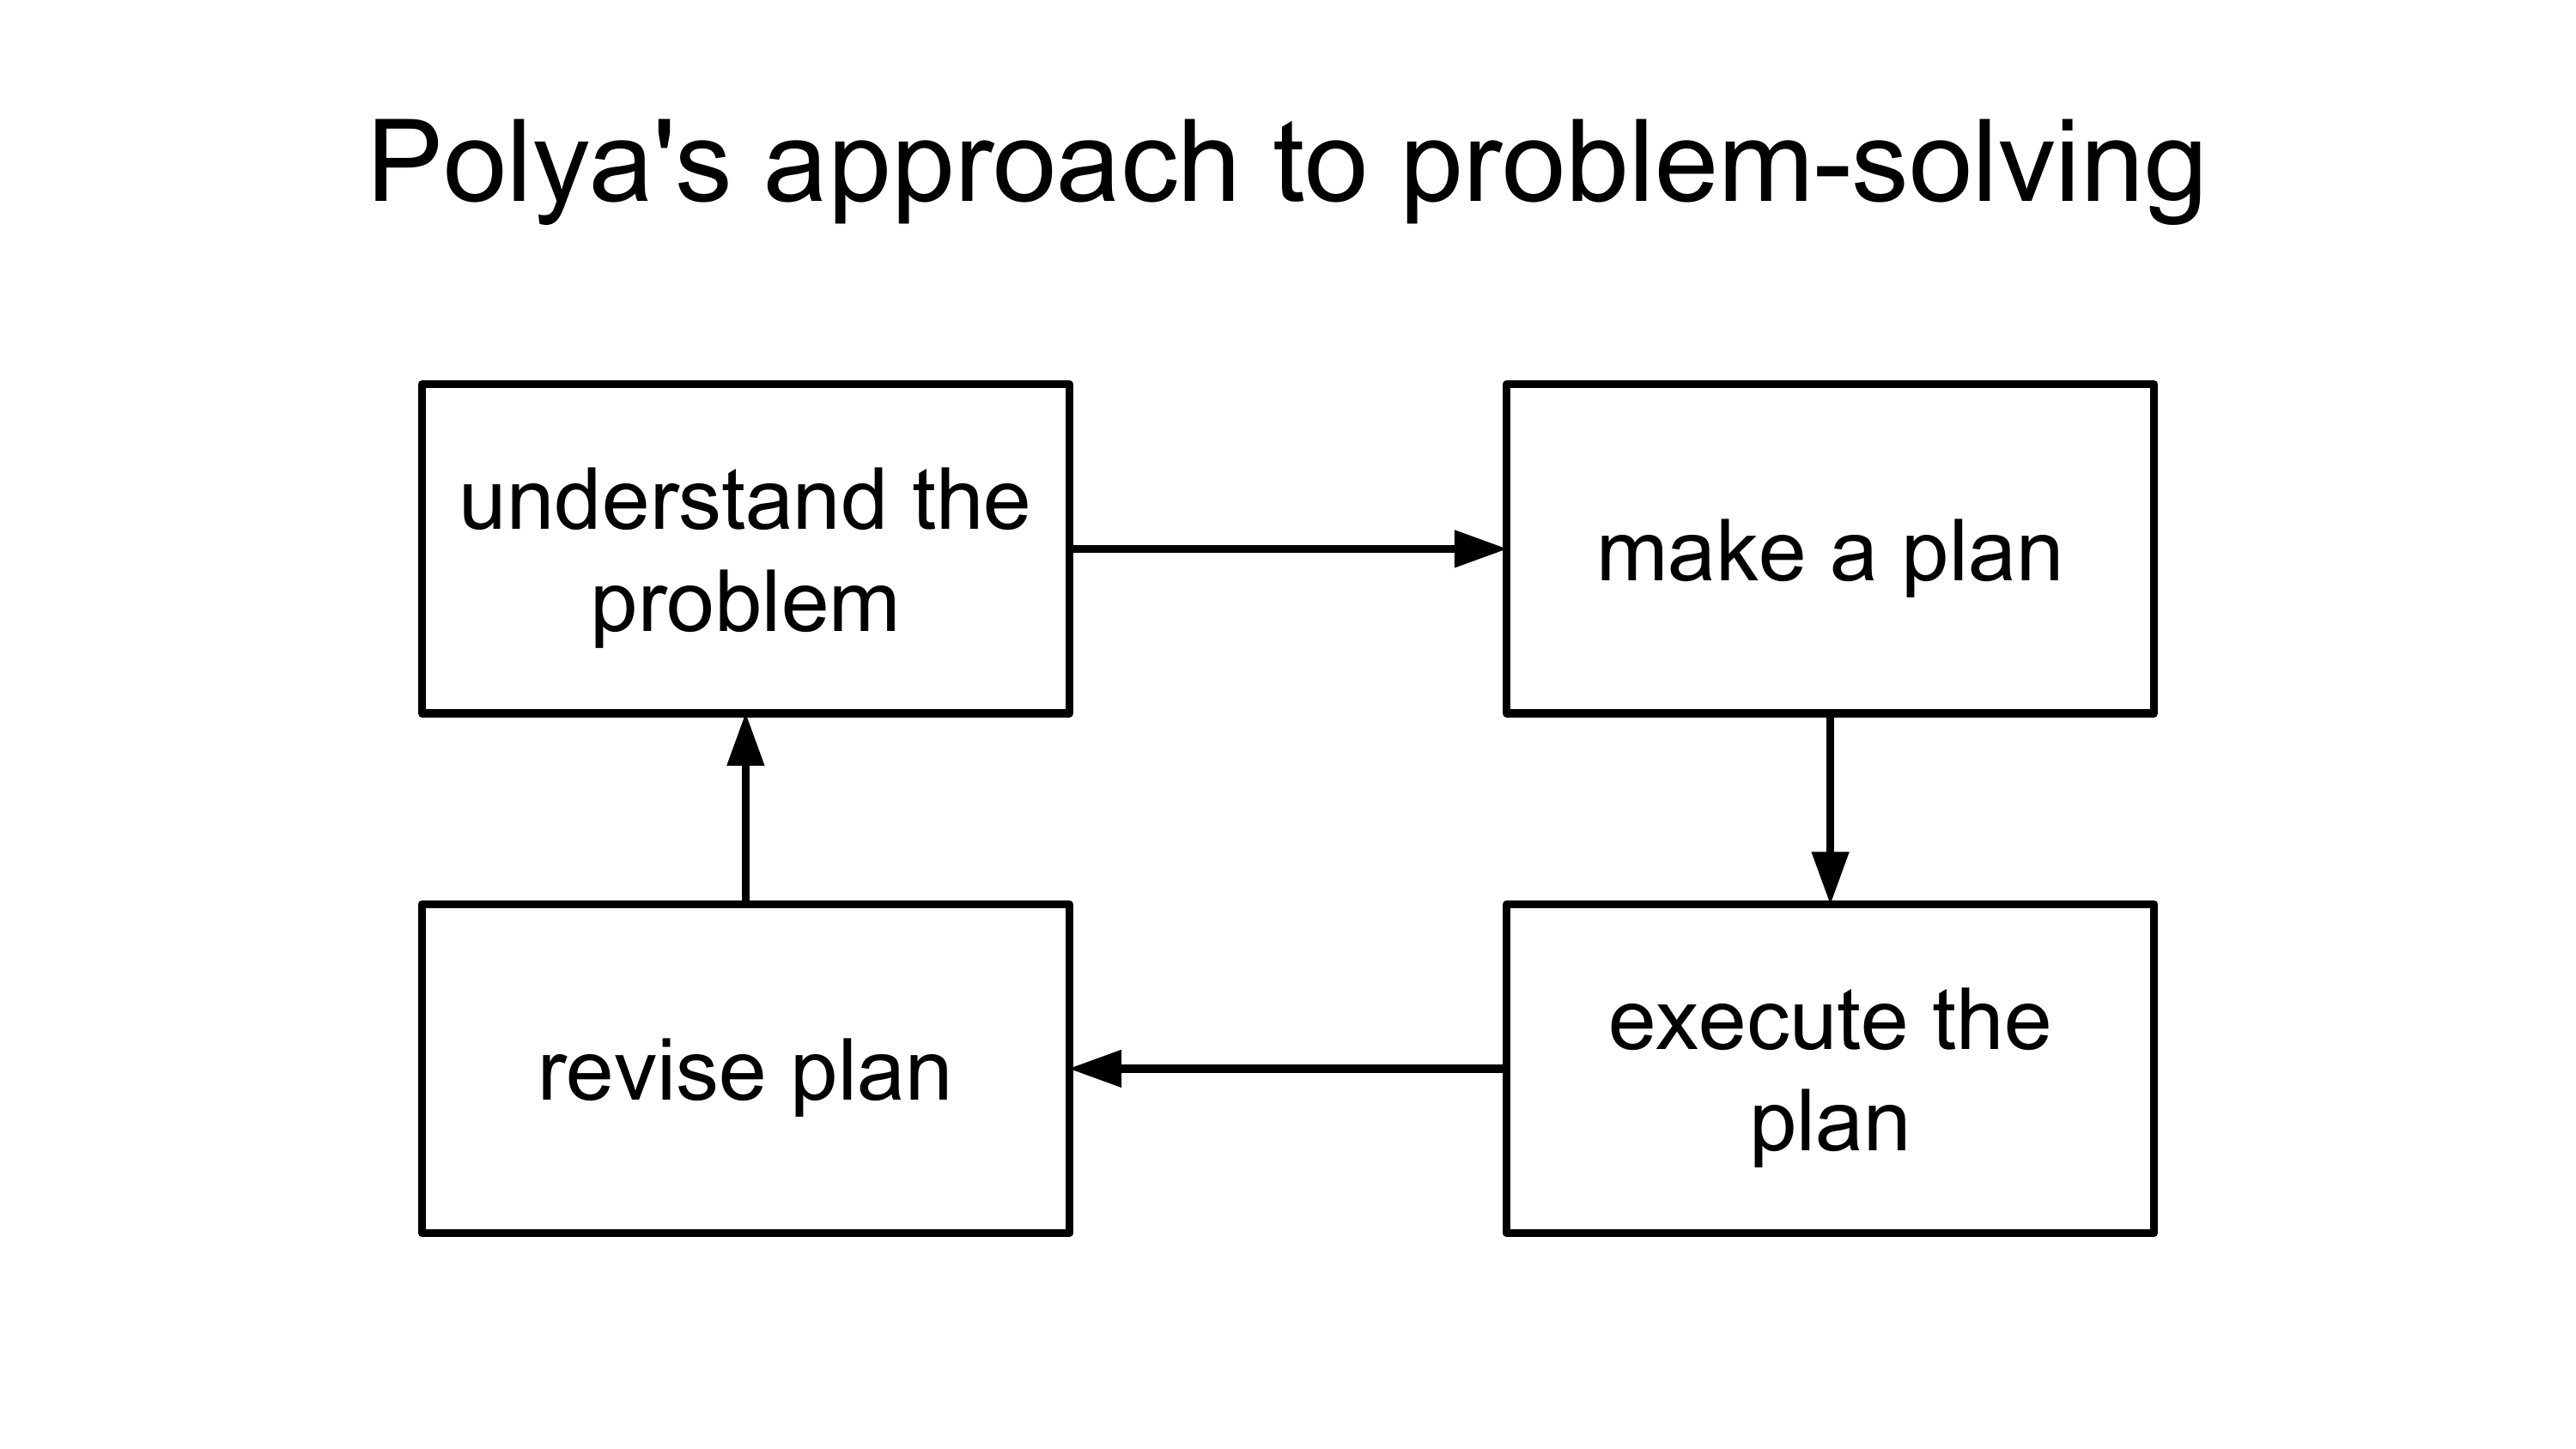
\includegraphics[width=1\linewidth,height=\textheight,keepaspectratio]{problem-solving_files/mediabag/problem_solving_poly.png}

}

\caption{\label{fig-polya}Der Ansatz von Polya zum Lösen von Problemen.}

\end{figure}%

Bevor wir uns mit dem oben genannten EVA-Modell beschäftigen, das uns
hilft, Probleme adäquat für Computer zu beschreiben, wollen wir einen
kurzen Blick auf eine andere Frage werfen: Warum überhaupt Computer zur
Problemlösung?

\section{Warum sind Computer beim Lösen von Problemen
nützlich?}\label{warum-sind-computer-beim-luxf6sen-von-problemen-nuxfctzlich}

Der wichtigste Grund für die Nutzung von Computern ist das Lösen von
Problemen. Ob wir eine Route mit Google Maps planen, Online-Bestellungen
bei DHL verfolgen oder eine KI wie ChatGPT um eine Empfehlung bitten --
überall lösen Computer Probleme. Warum? Weil Computer zwei Eigenschaften
besitzen, die für viele Probleme und deren Lösung vorteilhaft sind:

\begin{enumerate}
\def\labelenumi{\arabic{enumi}.}
\tightlist
\item
  Computer machen keine Fehler. Wenn wir einem Computer einen Lösungsweg
  beibringen, wendet er ihn fehlerfrei auf neue Probleme an.
\item
  Computer sind unglaublich schnell. Ob einfache Schritte, komplexe
  Berechnungen oder die Verarbeitung großer Datenmengen -- Computer
  lösen Probleme in einem Bruchteil der Zeit, die wir Menschen benötigen
  würden.
\end{enumerate}

Diese beiden Eigenschaften ermöglichen es uns, mit Computern besonders
solche Probleme effizient zu lösen, die wiederkehrend und in großer Zahl
auftreten. Wir sprechen dann von \textbf{Automatisierung}.

In diesem Abschnitt lernen wir, wie Computer Probleme strukturieren und
lösen. Um den Begriff des Problems besser zu verstehen und seine
Bedeutung im Kontext von Computern einzugrenzen, führen wir zunächst ein
einfaches Modell ein.

\section{Wie stellen wir Probleme für Computer
dar?}\label{sec-eva-model}

Ein Programm zu schreiben stellt eine komplexe Herausforderung dar. Beim
Lesen einer Aufgabenstellung, die man als Programm umsetzen soll, kann
man sich schnell überfordert fühlen. Die zentrale Frage lautet: Wie
nähern wir uns dieser Aufgabe systematisch an?

Ein bewährter Ansatz für komplexe Situationen ist die Vereinfachung.
Auch wenn wir das Problem selbst nicht vereinfachen können, können wir
es durch eine strukturierte Herangehensweise besser verstehen und
handhabbarer machen. Die Verwendung von Modellen ist dafür ein
geeigneter Weg.

Modelle zielen darauf ab, die wesentlichen Aspekte der realen Welt
hervorzuheben und unwichtige Details auszublenden. Da dies zunächst
abstrakt klingen mag, werden wir es anhand eines Modells
veranschaulichen, das uns durch das gesamte Buch begleiten wird: das
Eingabe-Verarbeitung-Ausgabe-Modell, kurz EVA-Modell.

\subsection{Das
Eingabe-Verarbeitung-Ausgabe-Modell}\label{das-eingabe-verarbeitung-ausgabe-modell}

Das Eingabe-Verarbeitung-Ausgabe-Modell (EVA-Modell, s.
Abbildung~\ref{fig-input-computation-output}) ist ein wichtiges Modell
in der Informatik. Es erklärt die Arbeitsweise von Computern auf
vereinfachte Weise und beinhaltet nur die nötigsten Elemente. Konkret
zeigt das Modell, wie Computer Probleme lösen und welche drei Elemente
wir dabei betrachten müssen: Computer benötigen \textbf{(1)
Eingabedaten}, die sie durch einen definierten \textbf{(2)
Verarbeitungsprozess} in gewünschte \textbf{(3) Ausgabendaten}
umwandeln.

Das EVA-Modell beschreibt ein Problem und dessen Lösung durch drei
Komponenten: die Eingabe (\emph{Input}), die der Computer erhält, die
Verarbeitung (\emph{Computation}), die er mit diesen Daten durchführt,
und die Ausgabe (\emph{Output}), die er als Ergebnis liefert. Wenn wir
diese drei Komponenten beschreiben können, haben wir die für den
Computer relevanten Aspekte des Problems erfasst -- alles andere ist
unwichtig.

\begin{figure}

\centering{

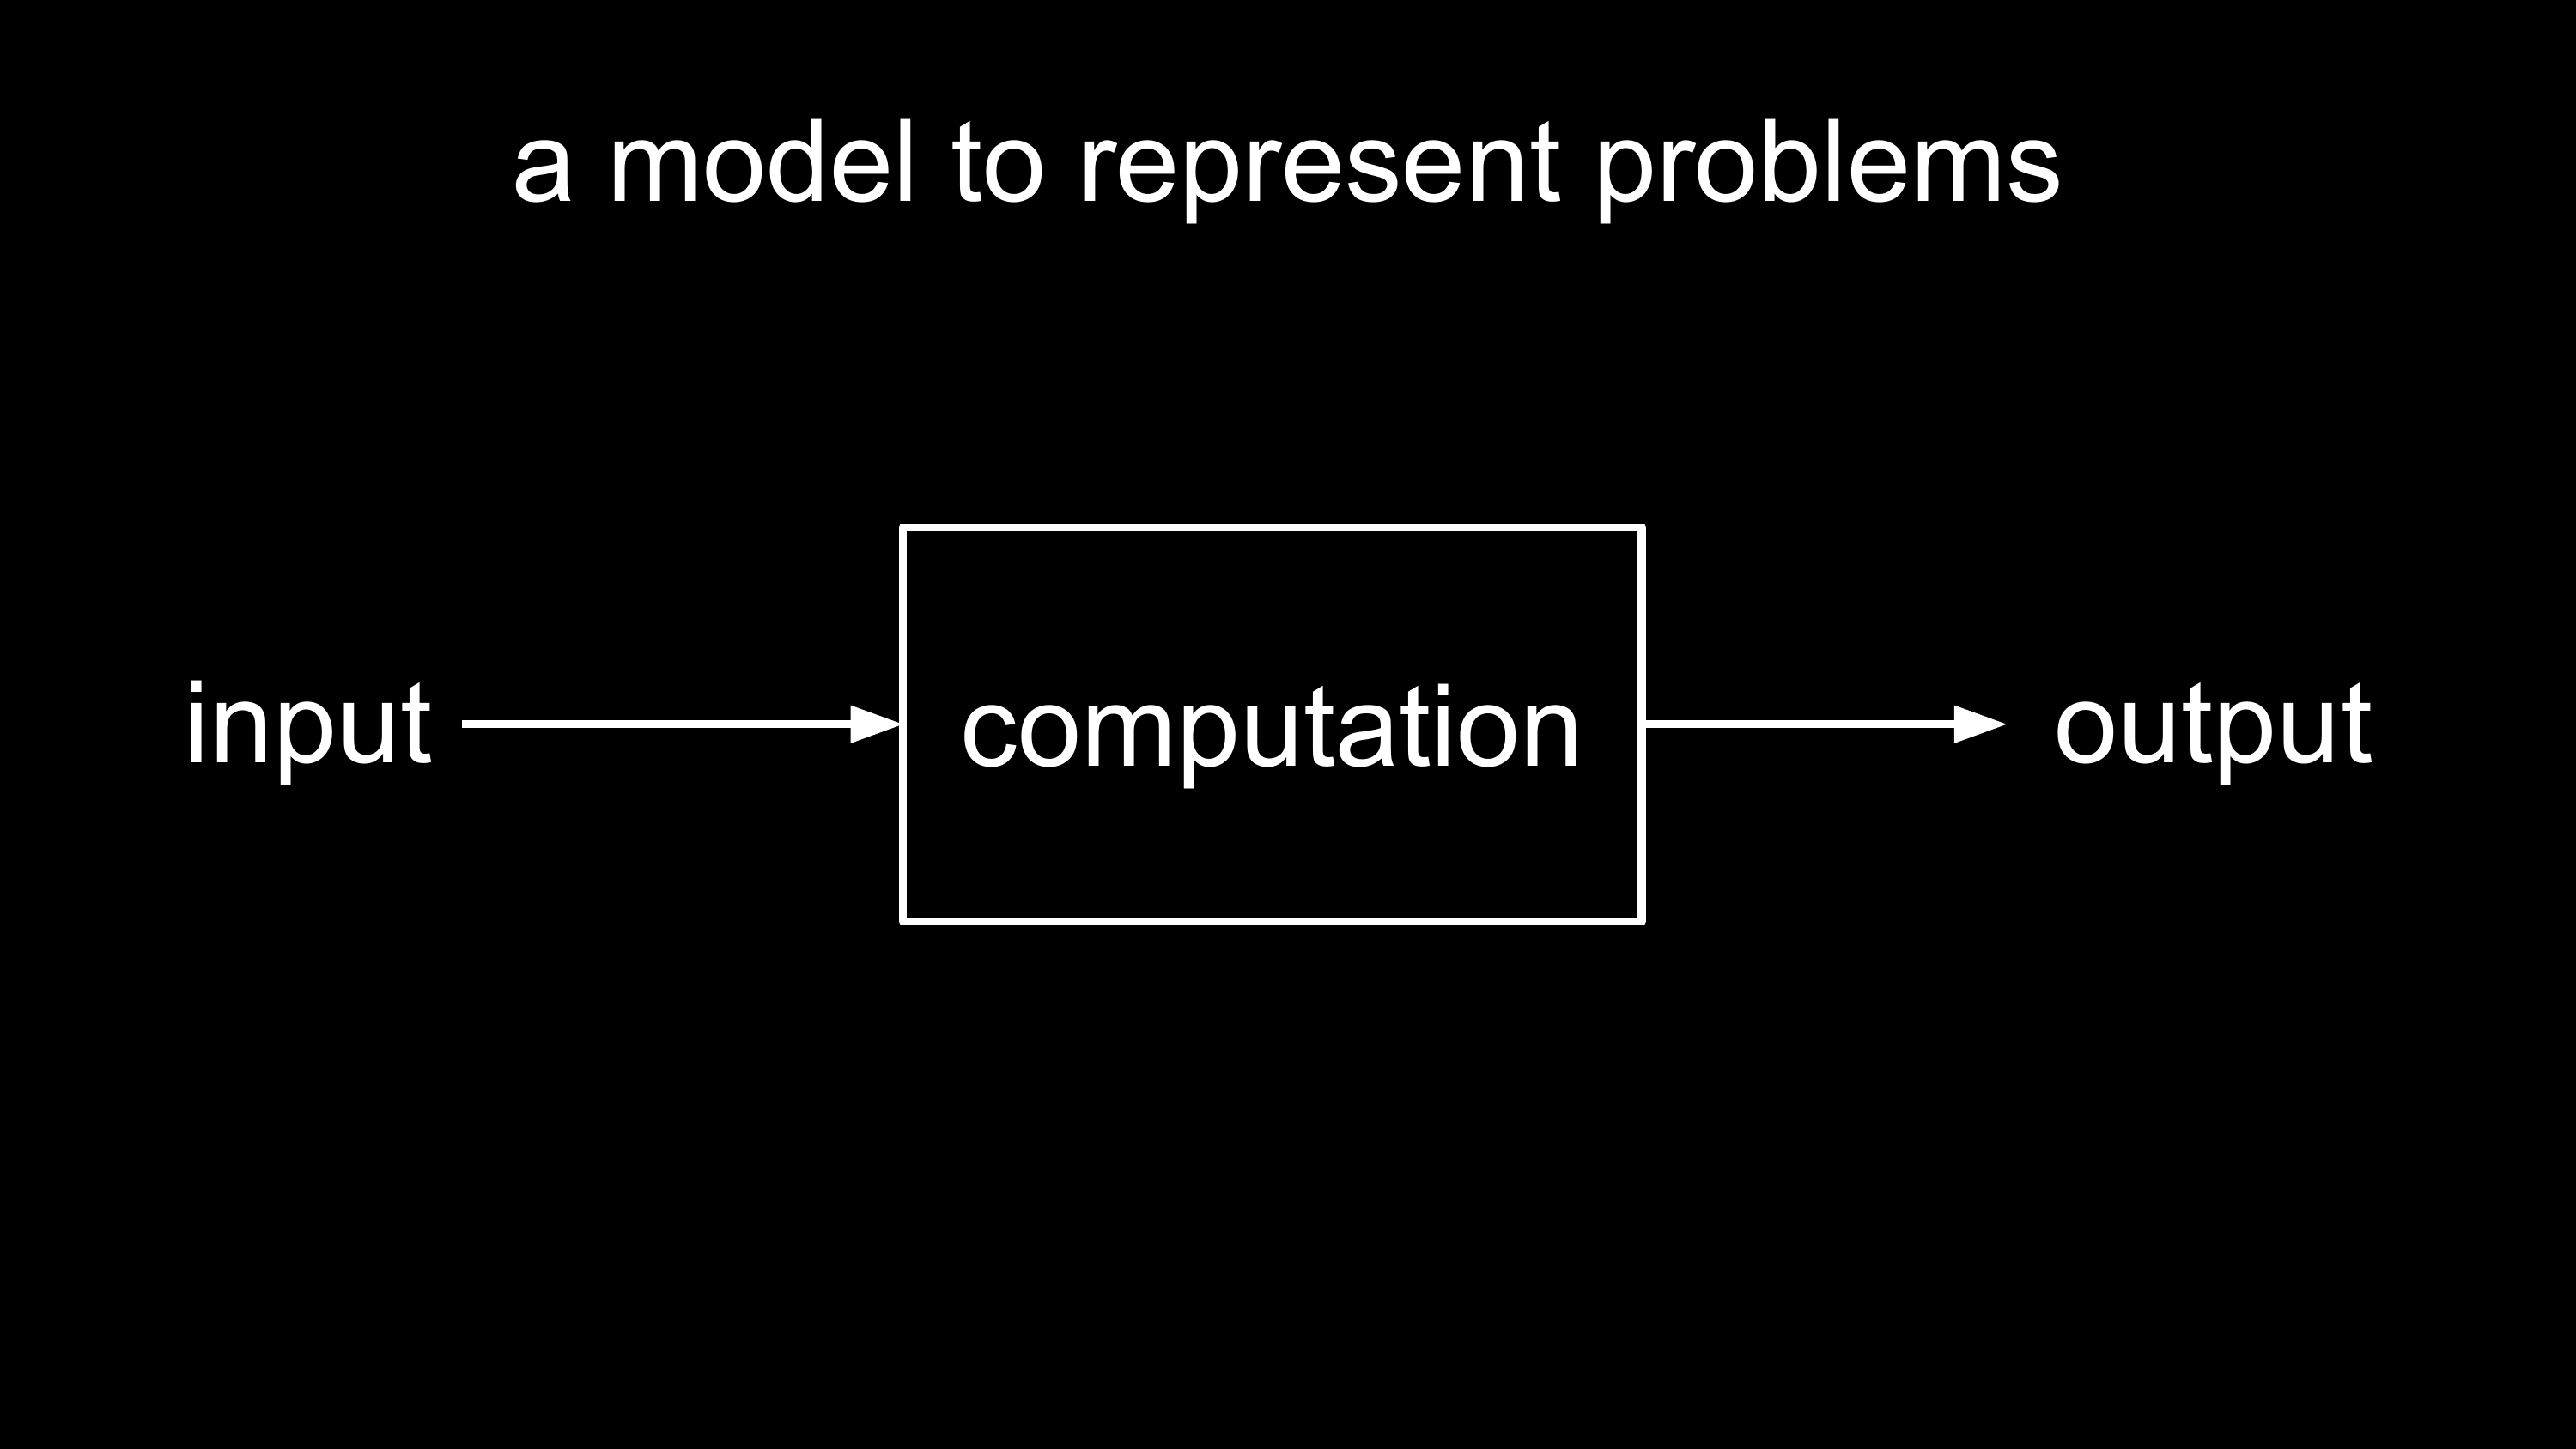
\includegraphics[width=1\linewidth,height=\textheight,keepaspectratio]{problem-solving_files/mediabag/problem_solving_inpu.png}

}

\caption{\label{fig-input-computation-output}Das EVA-Modell besteht aus
der Eingabe, der Berechnung und der Ausgabe.}

\end{figure}%

Wenden wir das EVA-Modell auf das Experiment zum LED-Regenbogenverlauf
an. Die LED muss durch ein Programm angesteuert werden, die Farben
sollen in einem bestimmten Ablauf verändert werden, so dass es das
Muster eines Regenbogens ergibt. Nehmen wir zudem an, dass die
Geschwindigkeit durch den Benutzer gesteuert werden soll. Wie ihr bei
der Durchführung des Experiments gemerkt habt, erfodert dieses scheinbar
einfache Probleme eine Menge von Teilschritten, die wir getrennt
voneinander umsetzen können. Dennoch können wir das EVA-Modell nutzen,
um das Expierment zunächst als Ganzes darzustellen, indem wir von den
Details der einzelnen Schritte abstrahieren:

\begin{center}
\includegraphics[width=1\linewidth,height=\textheight,keepaspectratio]{problem-solving_files/mediabag/problem_solving_inpu1.png}
\end{center}

Was haben wir nun dadurch gewonnen, dass wir das EVA-Modell angewendet
haben? Wir können uns nun auf die einzelnen Elemente konzentrieren und
diese getrennt voneinander betrachten. Damit zerlegen wir das große,
überfordernde Problem in kleinere Teile und machen es dadurch besser
beherrschbar.

Bei den Eingaben müssen wir uns fragen, wie diese konkret aussehen und
erfasst werden. Dabei geht es vor allem darum, in welcher Form die
Eingaben dem Computer vorliegen müssen, damit er sie verarbeiten kann.
Wie wird die Geschwindigkeit des Regenbogenverlaufs im Computer
dargestellt? Es geht also um die \textbf{Repräsentation von
Informationen}.

Sobald wir die Darstellung der Eingabe geklärt haben, können wir diese
als Grundlage für die Verarbeitung nutzen. Wie muss ein Programm
aussehen, das auf Basis der Eingabedaten die richtige Entscheidung
trifft? Welche Schritte sind notwendig? Welche Prüfungen muss das
Programm durchführen? Bei diesem Schritt geht es folglich um die
\textbf{Verarbeitung von Informationen}.

Schließlich müssen wir die Form der Ausgabe festlegen. Wie soll das
Verarbeitungsergebnis konkret aussehen? Da wir für die Kommunikation
wieder Lichtsignale verwenden, geht es auch bei der Ausgabe um die
\textbf{Repräsentation von Informationen}. Im Beispiel des
Regenbogenverlauf also die Frage, wie Farben im Computer dargestellt
werden.

\subsubsection{Beispiel: Taschenrechner}\label{beispiel-taschenrechner}

Am Beispiel eines Taschenrechner lässt sich das EVA-Modell gut
darstellen. Wir können uns bildlich vorstellen, wie ein Mensch die
Eingabe tätigt und danach das Ergebnis abliest. Es ist wichtig zu
verstehen, dass Eingabe und Ausgabe sehr unterschiedliche Formen
annehmen können und keinesfalls nur über eine Tastatur erfolgen müssen.

Das Beispiel des Taschenrechners wird in
Abbildung~\ref{fig-example-calculator} anhand einer einfachen Addition
zweier Zahlen konkreter verdeutlicht. Als Eingabe werden zwei Zahlen
benötigt, die Berechnung erfolgt durch eine Addition, dargestellt durch
das Plussymbol. Die Ausgabe ist das Ergebnis -- die Summe.

\begin{figure}

\centering{

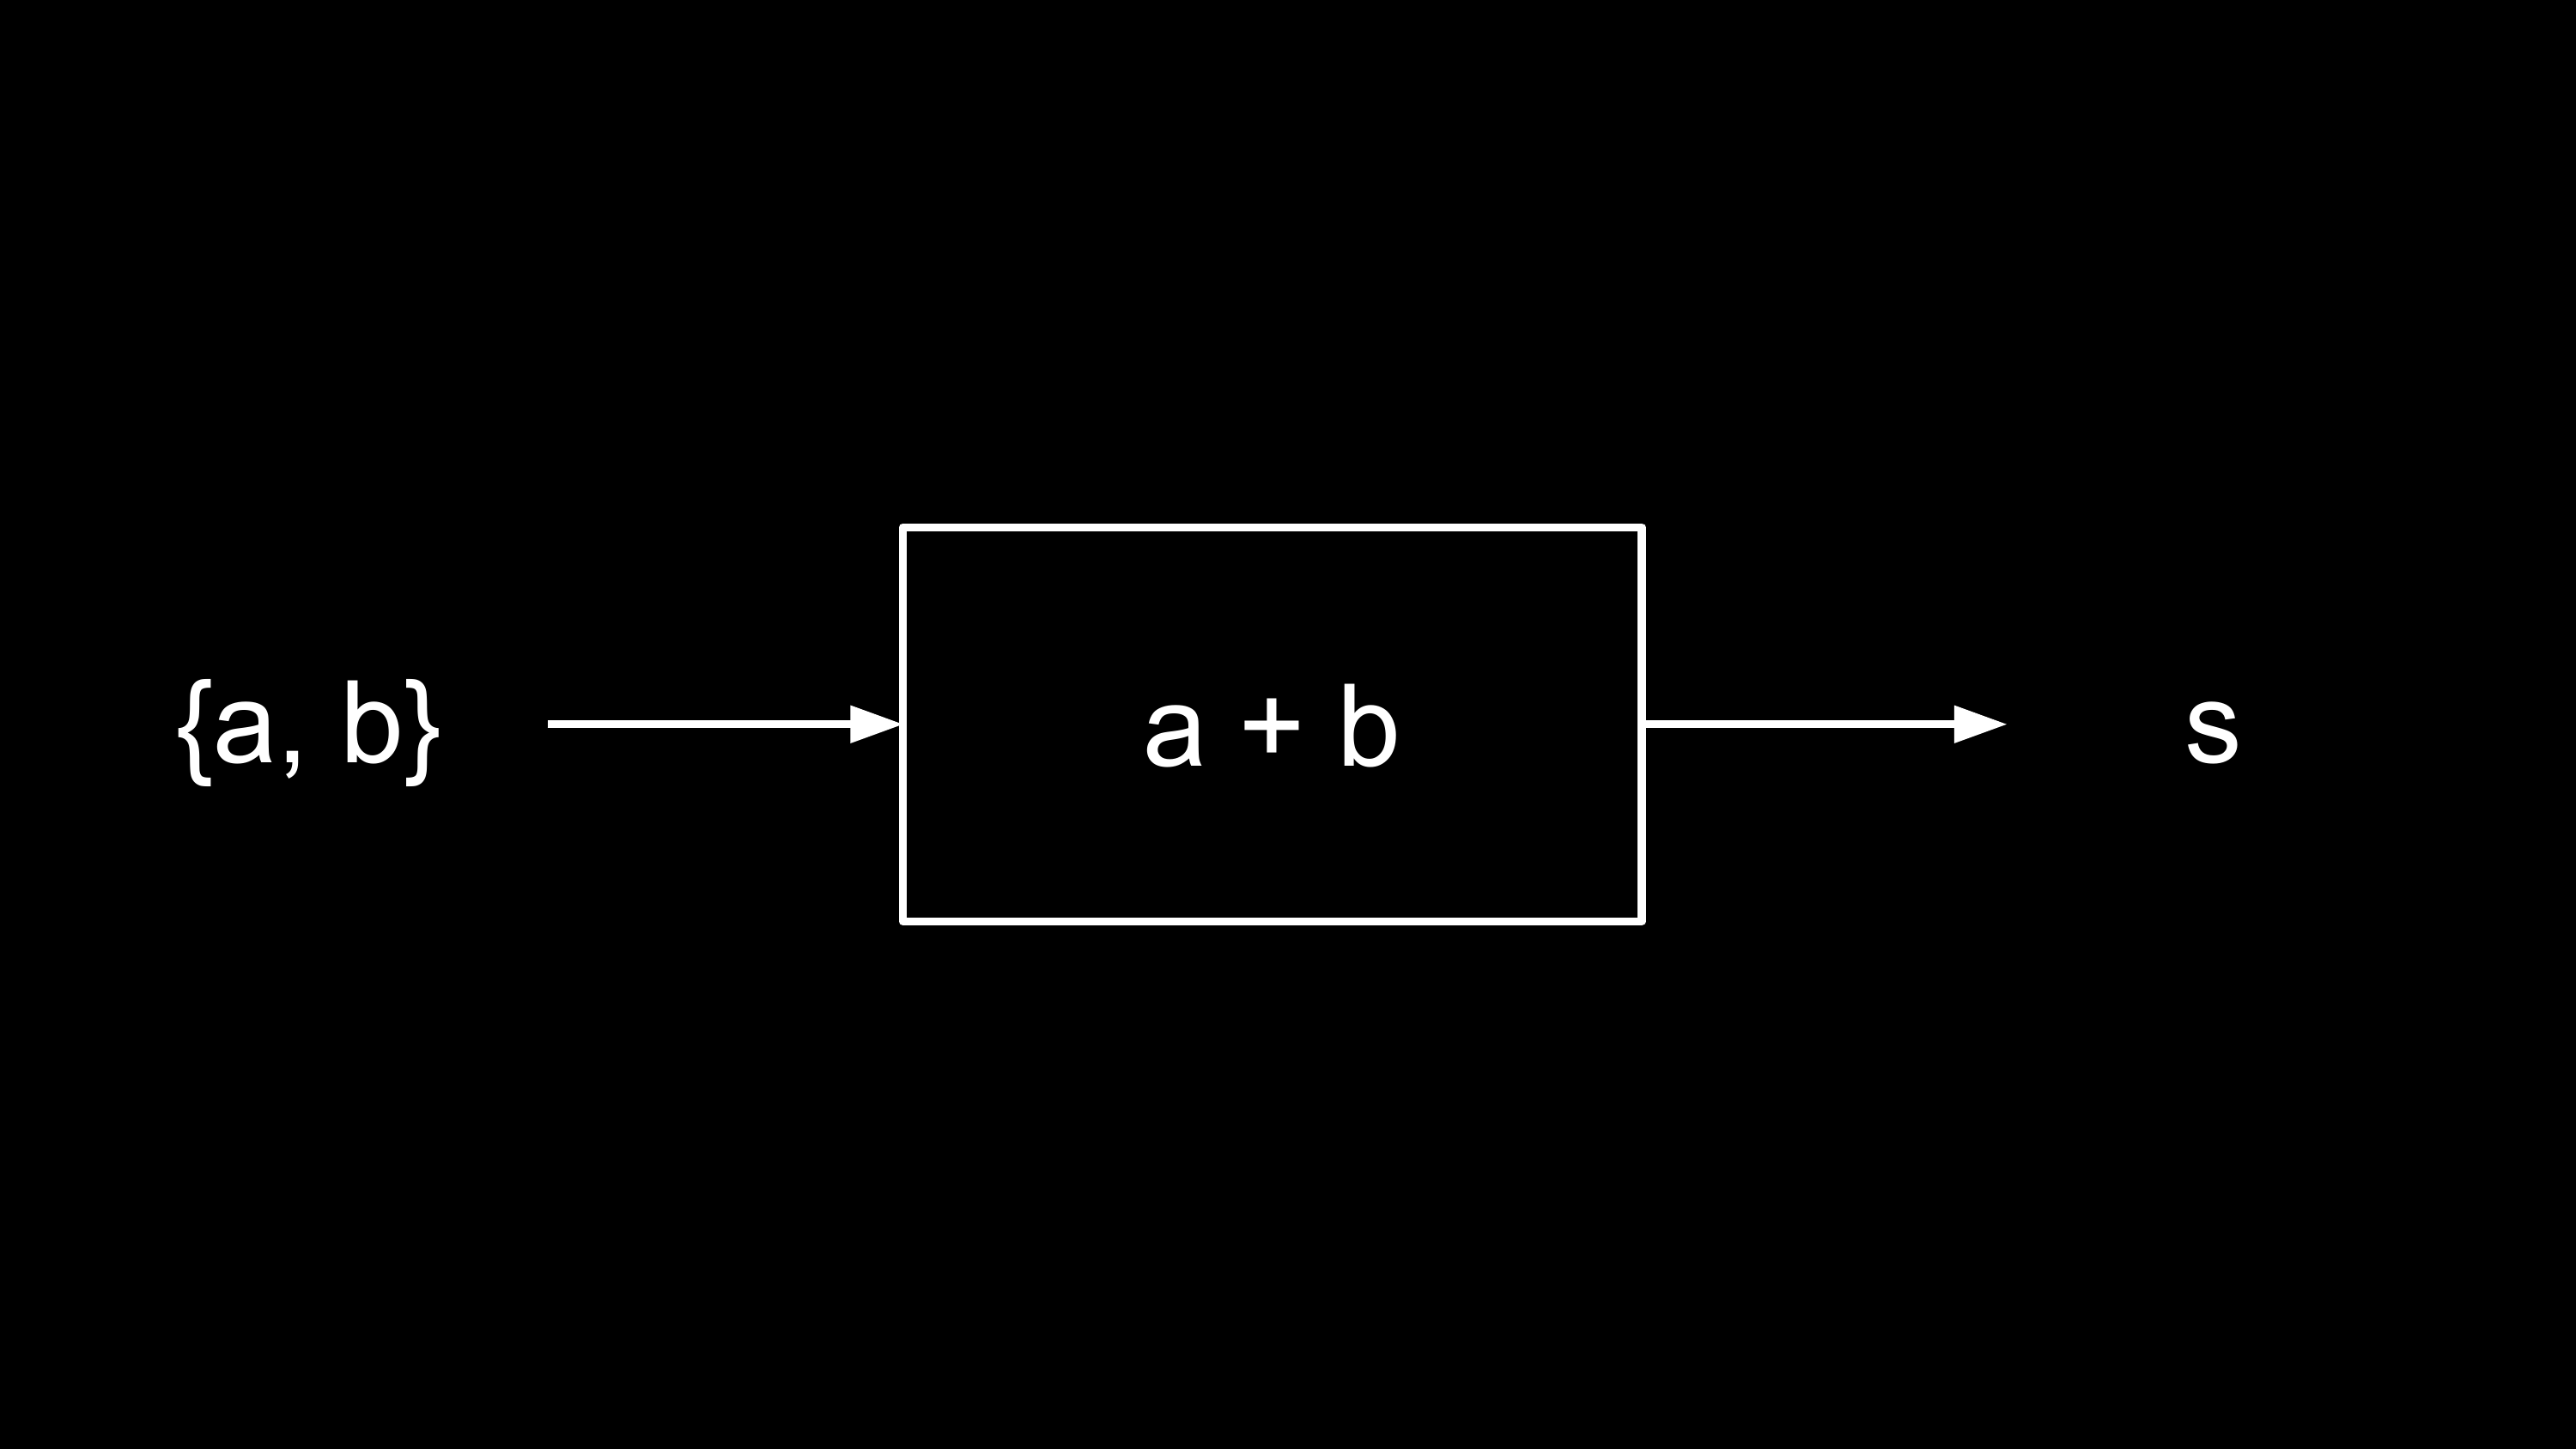
\includegraphics[width=1\linewidth,height=\textheight,keepaspectratio]{problem-solving_files/mediabag/problem_solving_exam.png}

}

\caption{\label{fig-example-calculator}Das EVA-Modell für die Addition
zweier Zahlen.}

\end{figure}%

Dieses einfache Beispiel zeigt, dass wir verstehen müssen, wie Computer
die drei Bestandteile des EVA-Modells umsetzen. Beim Taschenrechner sind
Ein- und Ausgabe jeweils Zahlen. Diese Daten speichert der Computer in
seinem Arbeitsspeicher. Dabei ist wichtig zu wissen, dass Computer auf
der untersten Ebene ausschließlich Nullen und Einsen speichern. Wir
müssen also verstehen, wie Computer Zahlen mithilfe dieser Binärzahlen
darstellen können.

Was passiert bei der Berechnung in der Mitte des Modells? Eine Addition
mag uns einfach erscheinen, doch auch hier müssen wir beachten, dass
Computer mit Binärzahlen arbeiten. Es stellt sich also die Frage: Wie
funktioniert eine Addition, wenn die Zahlen als Folge von Nullen und
Einsen dargestellt sind? Auf die beiden Fragen zur
\textbf{Repräsentation und der Verarbeitung von Informationen} im
binären System werden wir im Laufe des Buches Antworten bekommen.

\subsubsection{Beispiel: Pflanzen
zählen}\label{beispiel-pflanzen-zuxe4hlen}

Betrachten wir ein weiteres Beispiel: Stell dir vor, du möchtest einen
Computer nutzen, um Maispflanzen auf einer Drohnenaufnahme eines Ackers
zu zählen. Diese Aufgabe ist für Menschen zwar einfach zu verstehen,
wäre aber sehr zeitaufwändig auszuführen. Moderne Algorithmen
ermöglichen es Computern, Objekte auf Bildern präzise zu lokalisieren
und zu zählen. Nehmen wir an, wir haben für dieses Problem bereits eine
Lösung entwickelt und ein Programm namens \texttt{count\_plants}
erstellt. Nun stellt sich die Frage: Wie sehen die Eingabe und die
Ausgabe für dieses Problem aus? Was benötigt das Programm von uns, und
was liefert es als Ergebnis?

\begin{center}
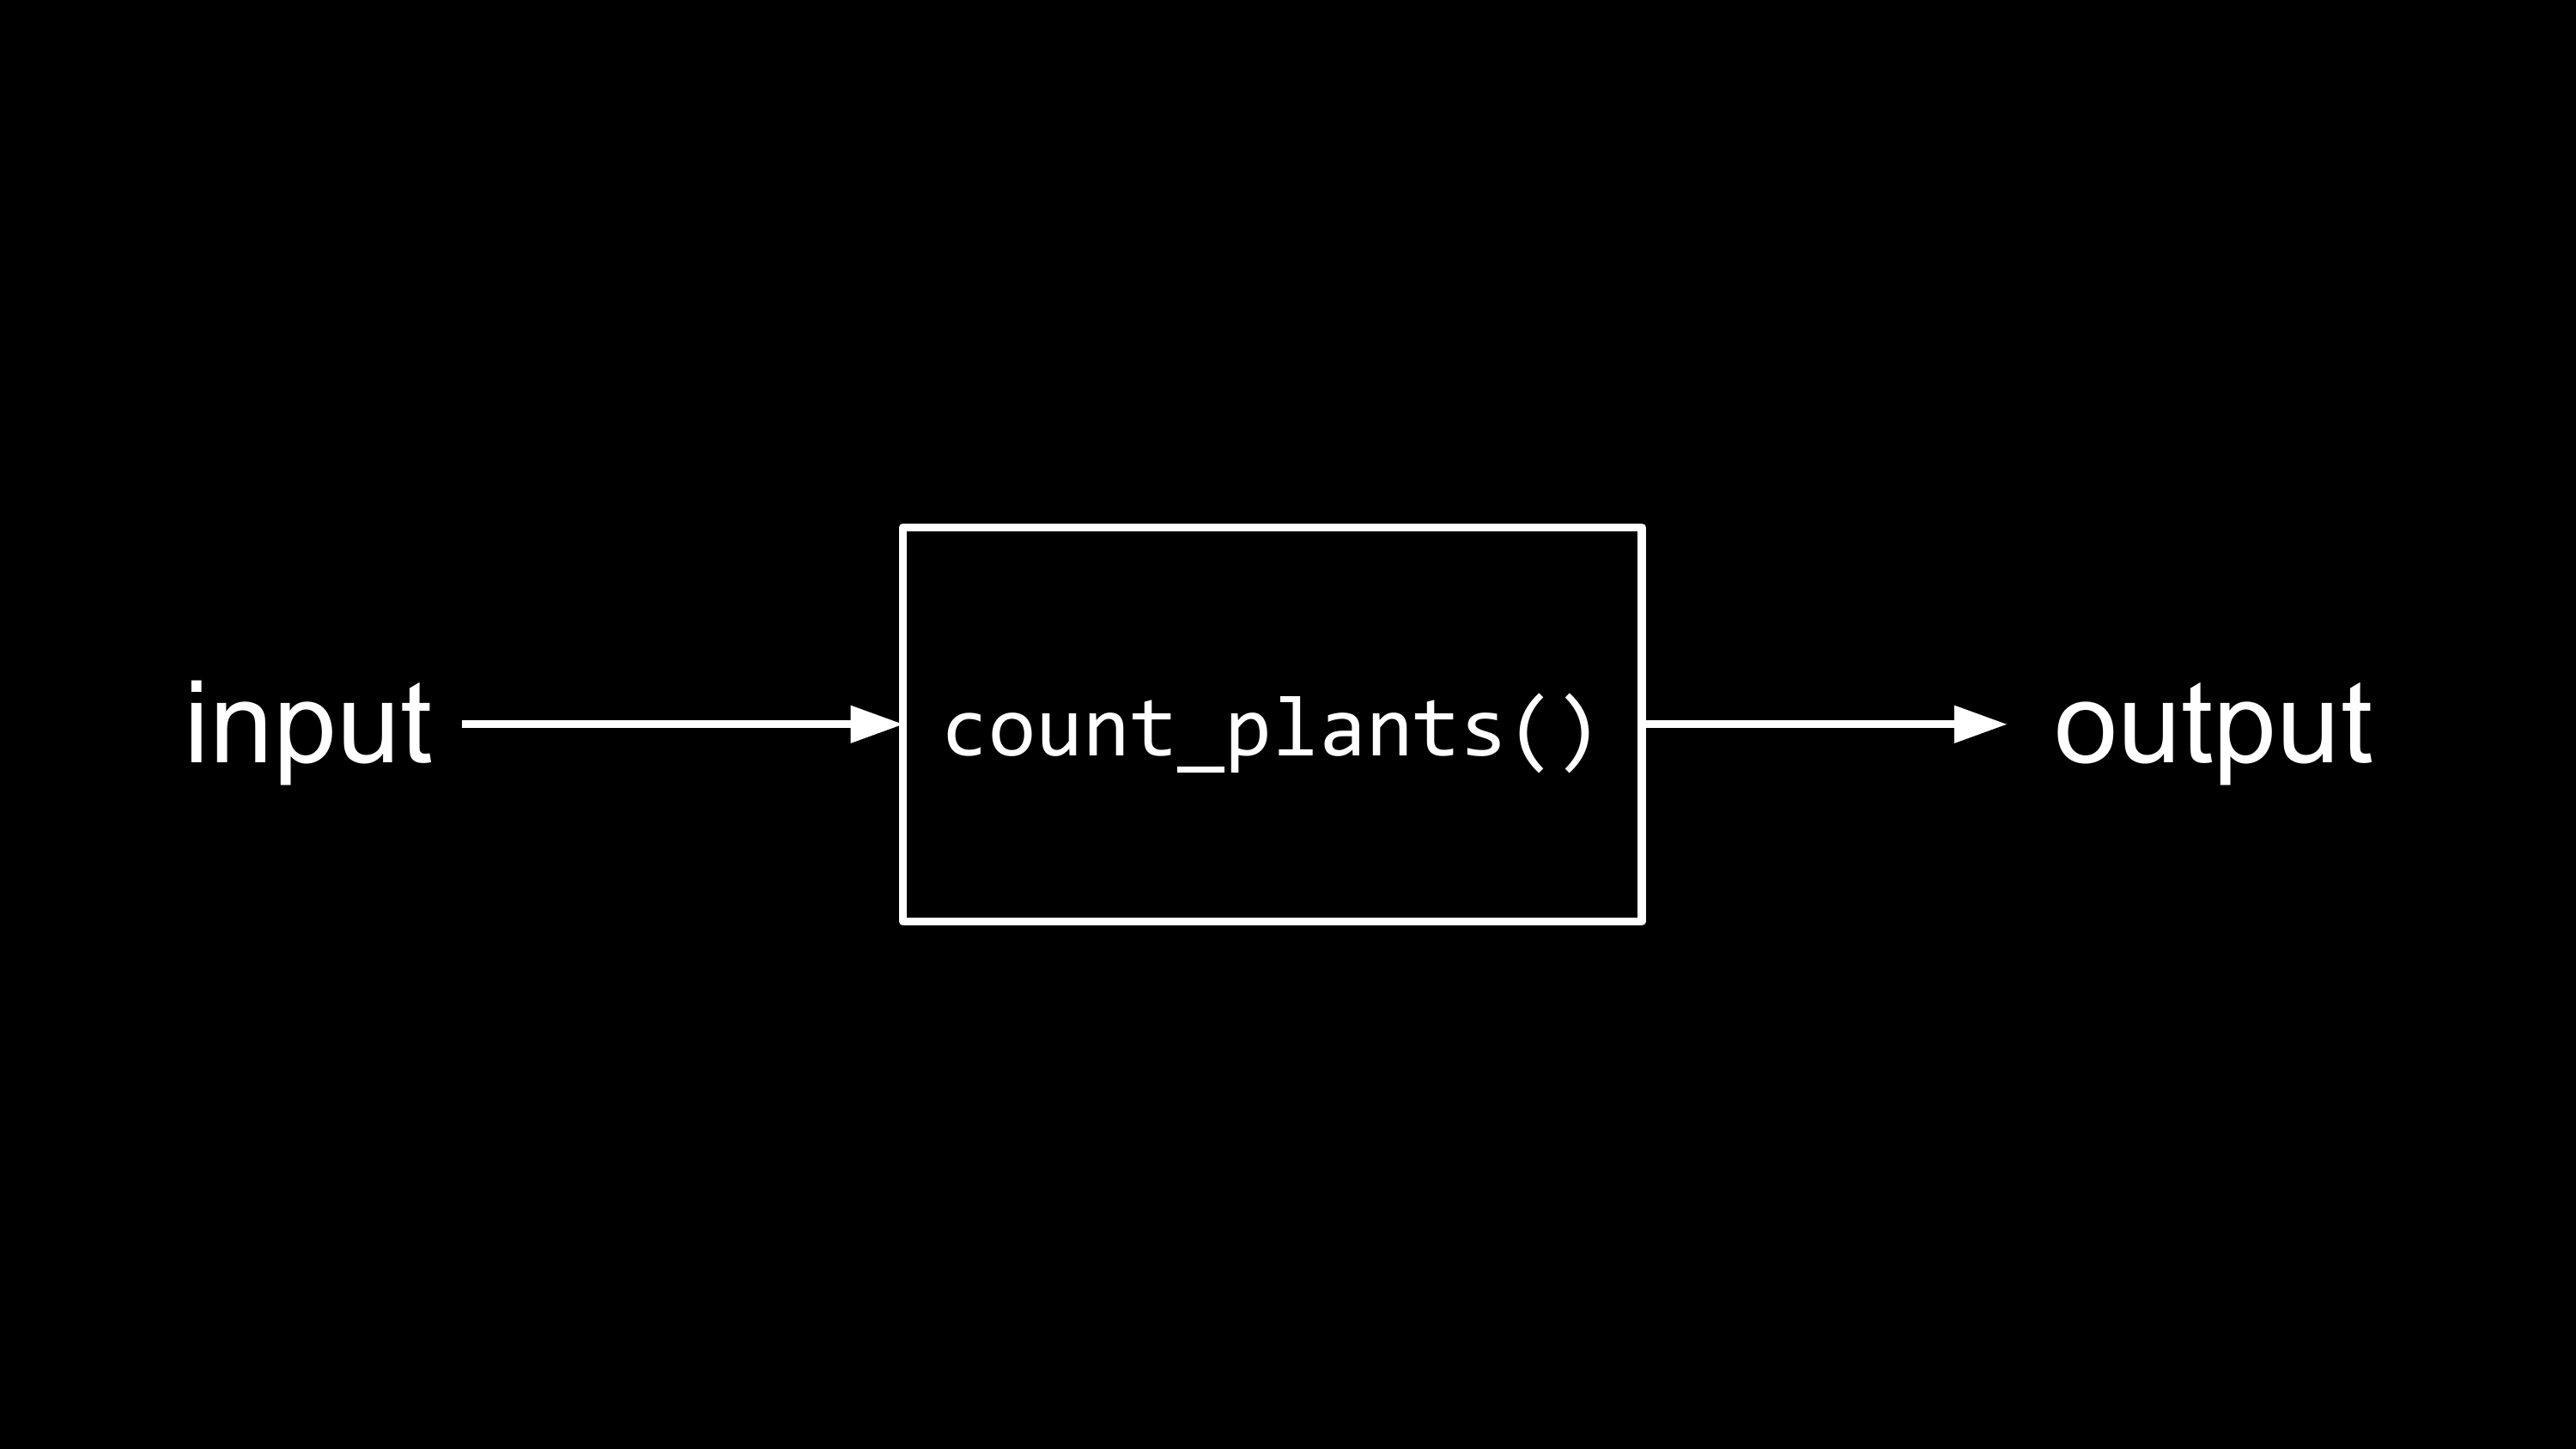
\includegraphics[width=1\linewidth,height=\textheight,keepaspectratio]{problem-solving_files/mediabag/problem_solving_exam1.png}
\end{center}

Die erwartete \textbf{Ausgabe} lässt sich einfach beschreiben: Das
Ergebnis der Zählung ist eine ganze Zahl. Die \textbf{Eingabe} für
dieses Problem ist - anders als beim Taschenrechner - kein Tastendruck,
sondern ein Bild. Damit der Computer das Bild verarbeiten kann, muss es
dem Computer in digitaler Form bereitgestellt werden. Was das genau
bedeutet, lernen wir in einem späteren Kapitel. Hier genügt es uns zu
verstehen, \emph{dass }wir das Bild digital abbilden müssen.

\begin{center}
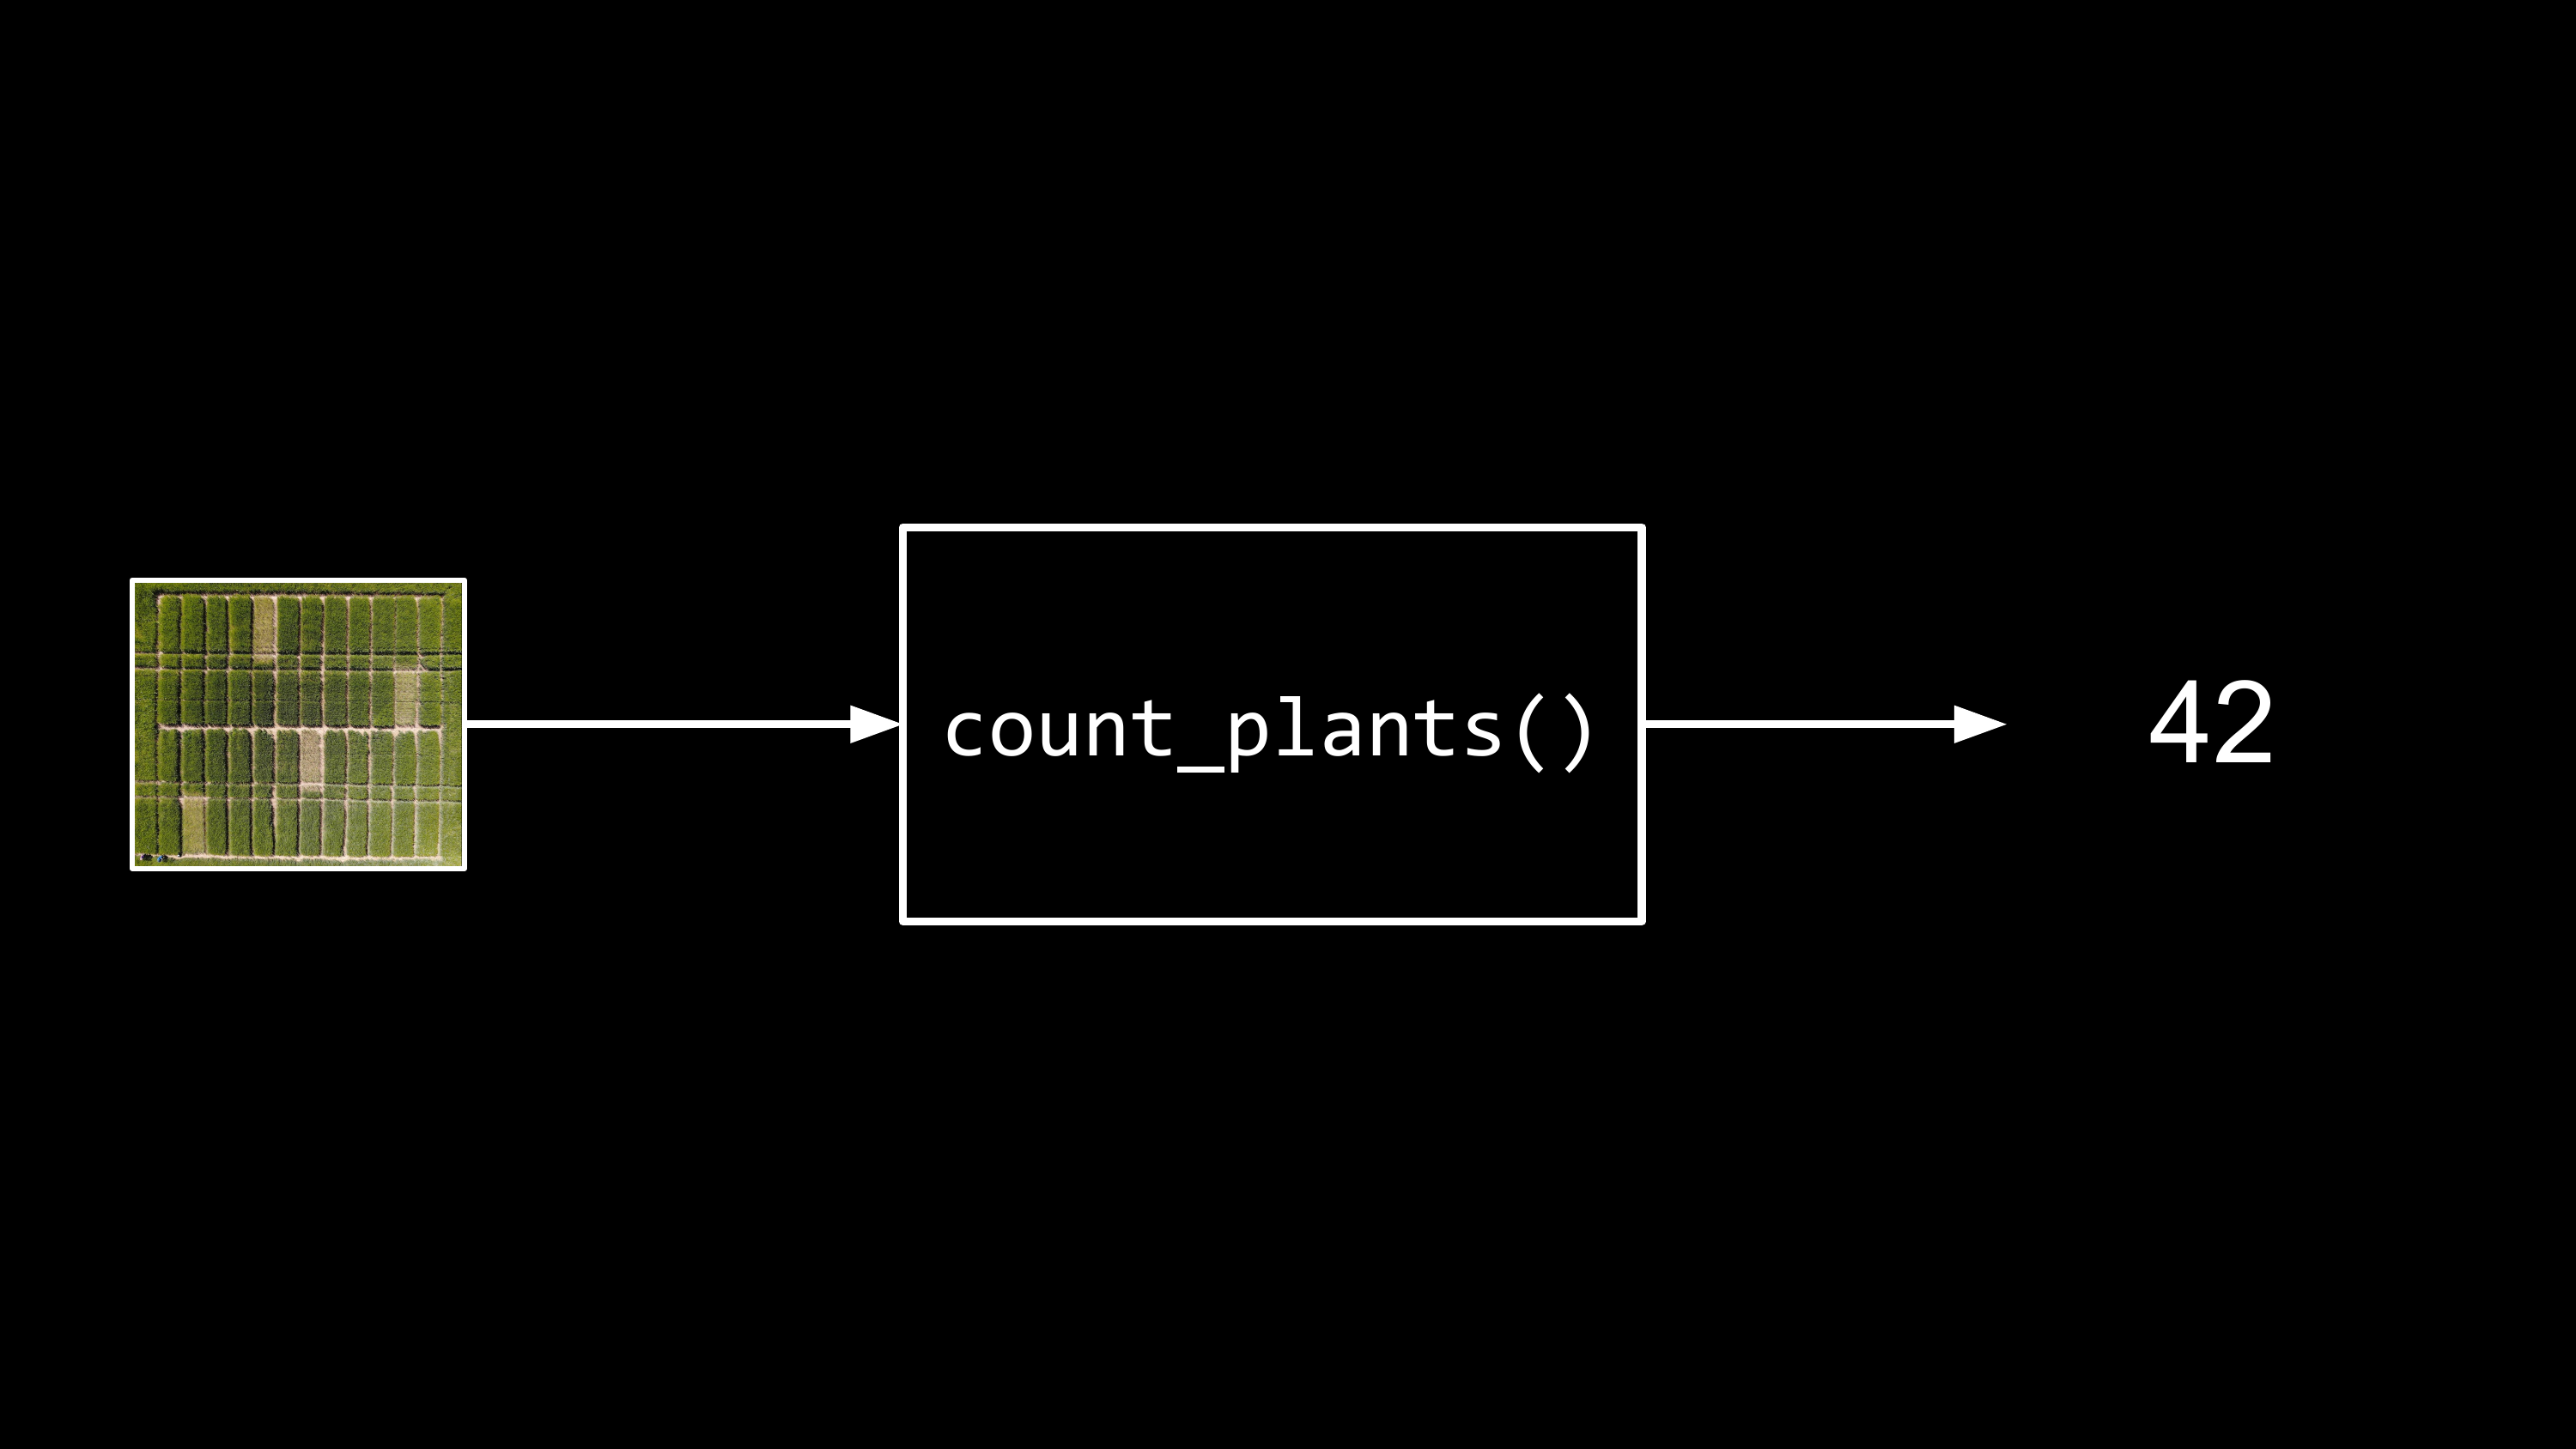
\includegraphics[width=1\linewidth,height=\textheight,keepaspectratio]{problem-solving_files/mediabag/problem_solving_exam12.png}
\end{center}

Wie gelangt das Bild in den Computer? Dies ist im Modell nicht näher
definiert und für die Problembeschreibung auch nicht wesentlich. Das
Bild muss lediglich irgendwie in den Arbeitsspeicher des Programms
\texttt{count\_plants} gelangen. Dies kann auf verschiedene Arten
geschehen: Es kann von der Festplatte gelesen werden, über eine
drahtlose Verbindung wie Bluetooth direkt übertragen und verarbeitet
werden, oder das Programm \texttt{count\_plants} läuft direkt auf der
Drohne und greift unmittelbar auf deren Kamera zu. Die technische
Umsetzung ist für unser Modell zunächst irrelevant. In einem späteren
Kapitel werden wir uns damit befassen, wie Informationen genau
übertragen und gespeichert werden. Genauso werden wir lernen, wie die
benötigten Informationen für die Ein- und Ausgabe eines Programms in
digitaler Form dargestellt werden können.

\begin{center}
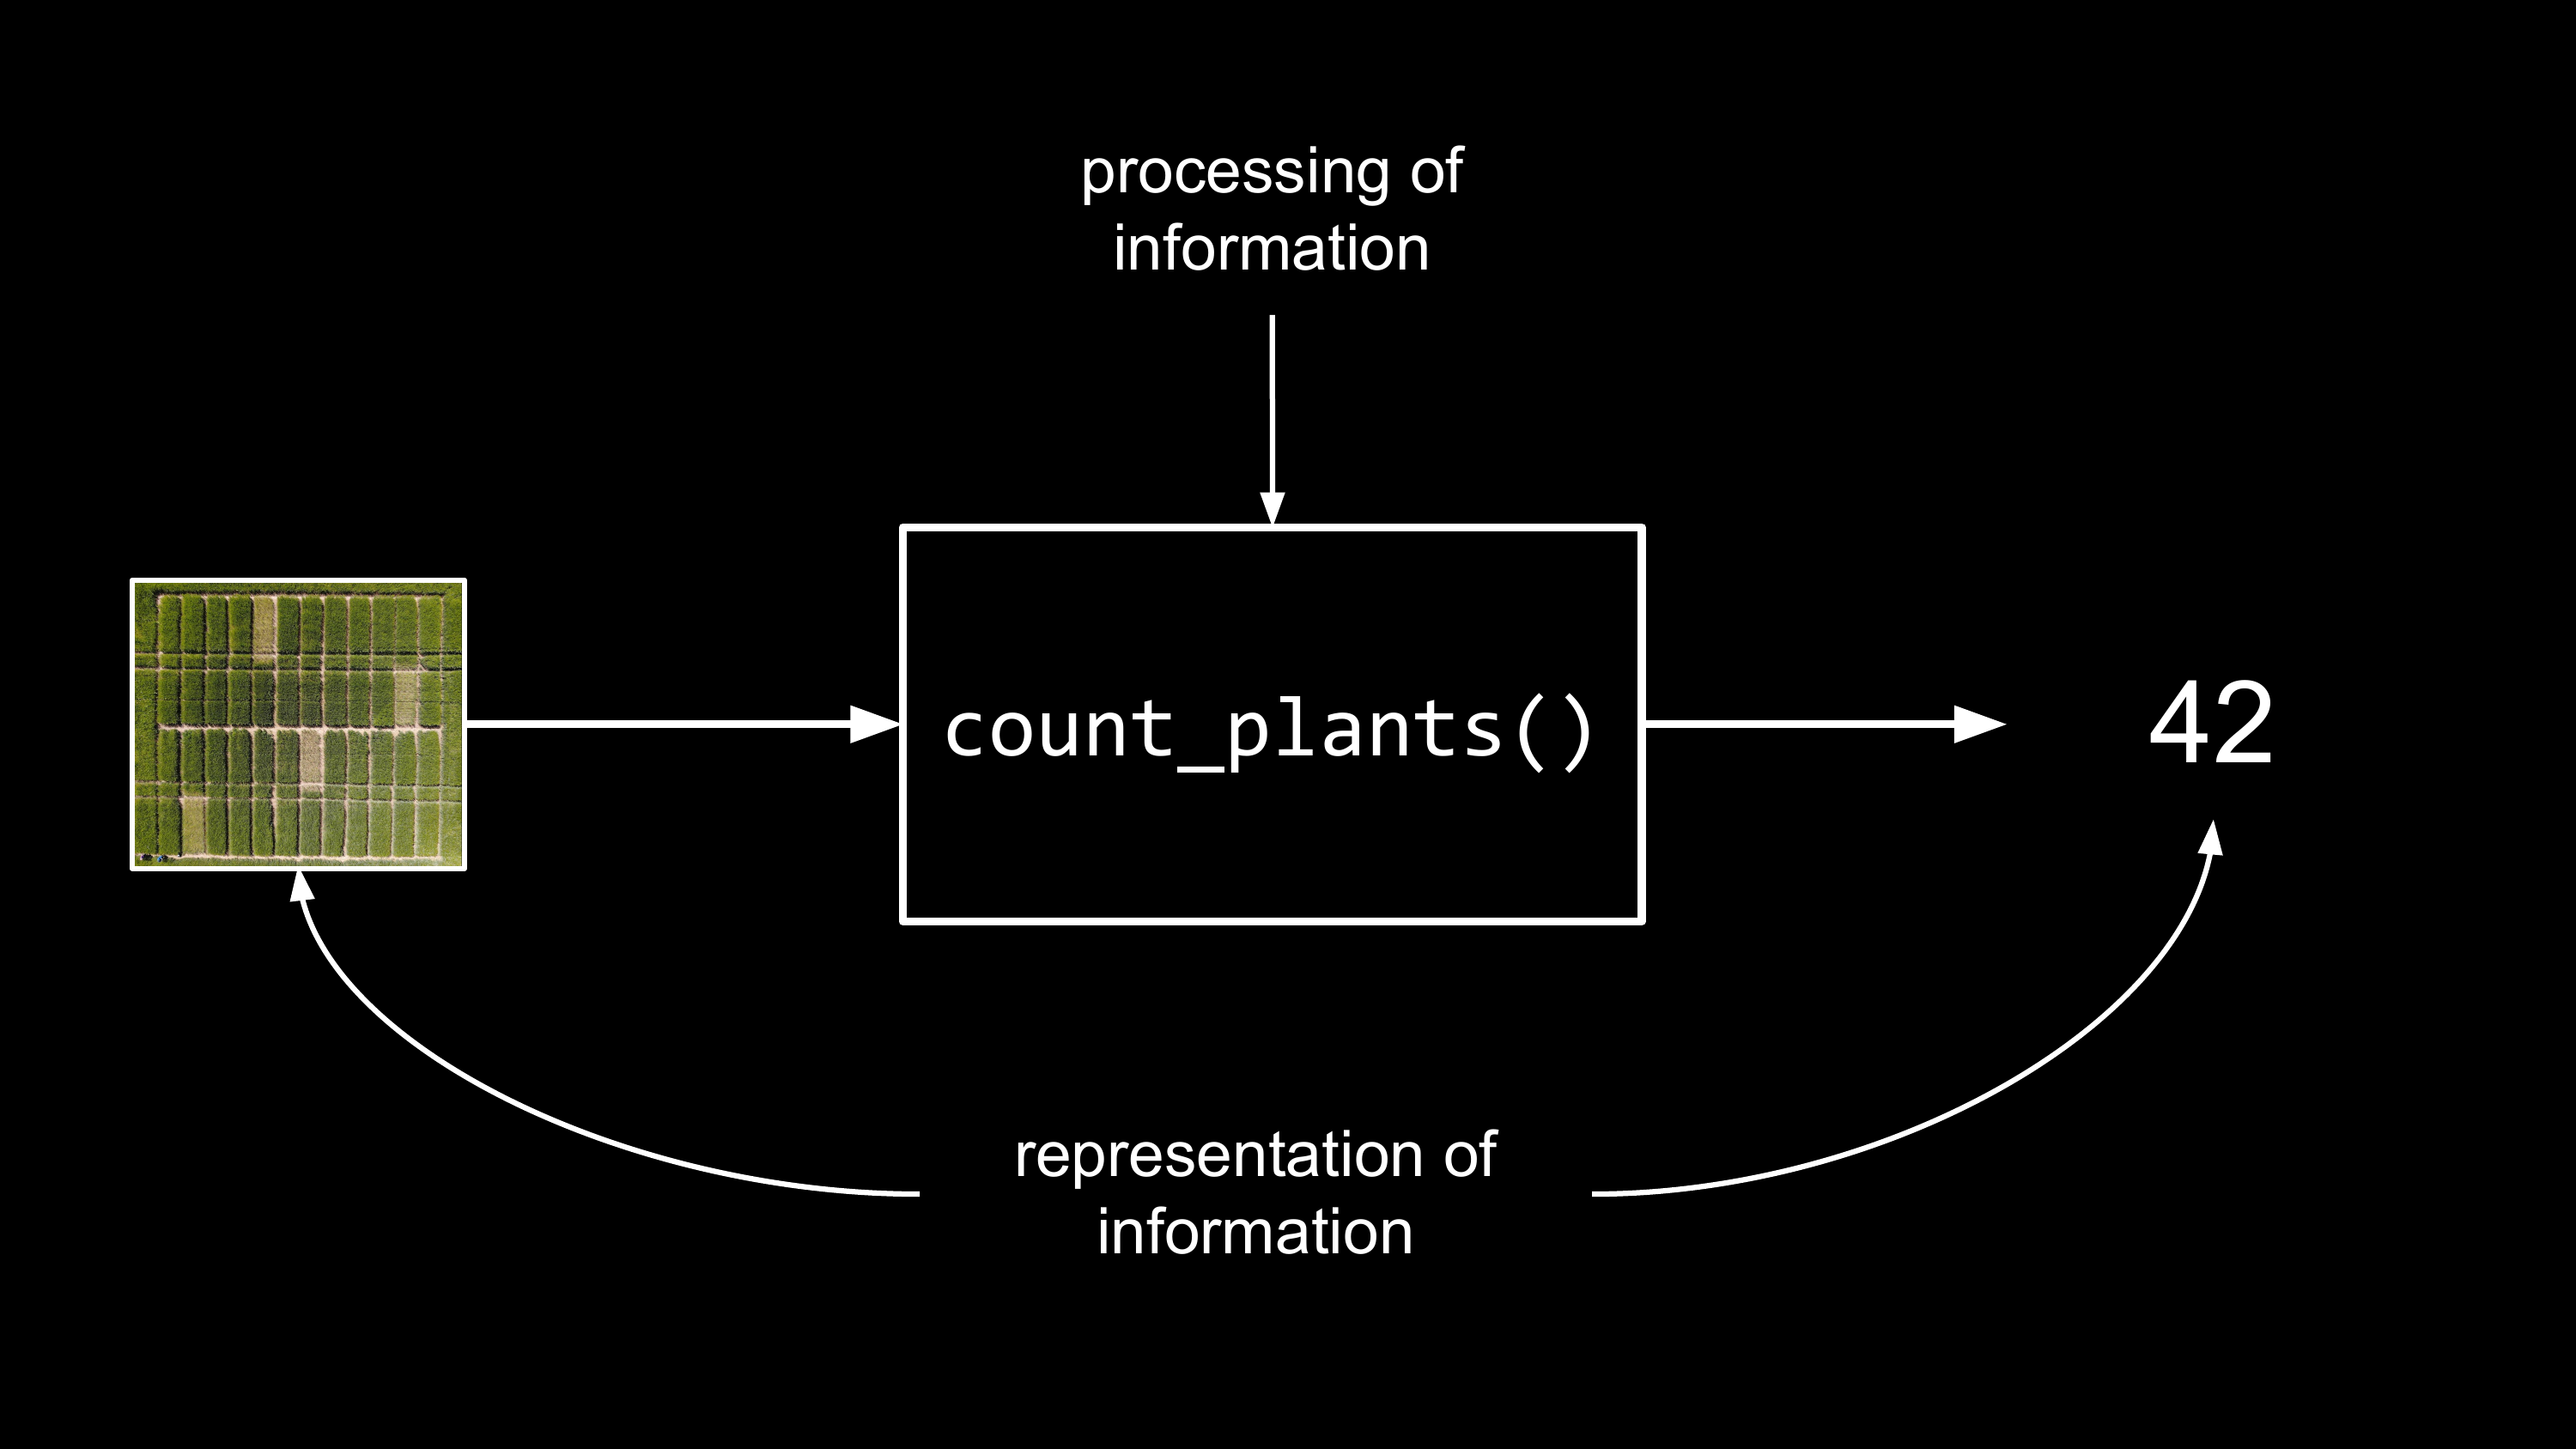
\includegraphics[width=1\linewidth,height=\textheight,keepaspectratio]{problem-solving_files/mediabag/problem_solving_exam123.png}
\end{center}

\subsubsection{Beispiel: Schach spielen}\label{beispiel-schach-spielen}

Ein weiteres Beispiel zur Verdeutlichung des EVA-Modells ist das
Schachspiel. Das Problem lässt sich einfach beschreiben: Der Computer
soll auf Grundlage einer bestehenden Spielsituation den bestmöglichen
nächsten Zug vorschlagen. Dieser Zug soll die Gewinnchancen maximieren.

\begin{center}
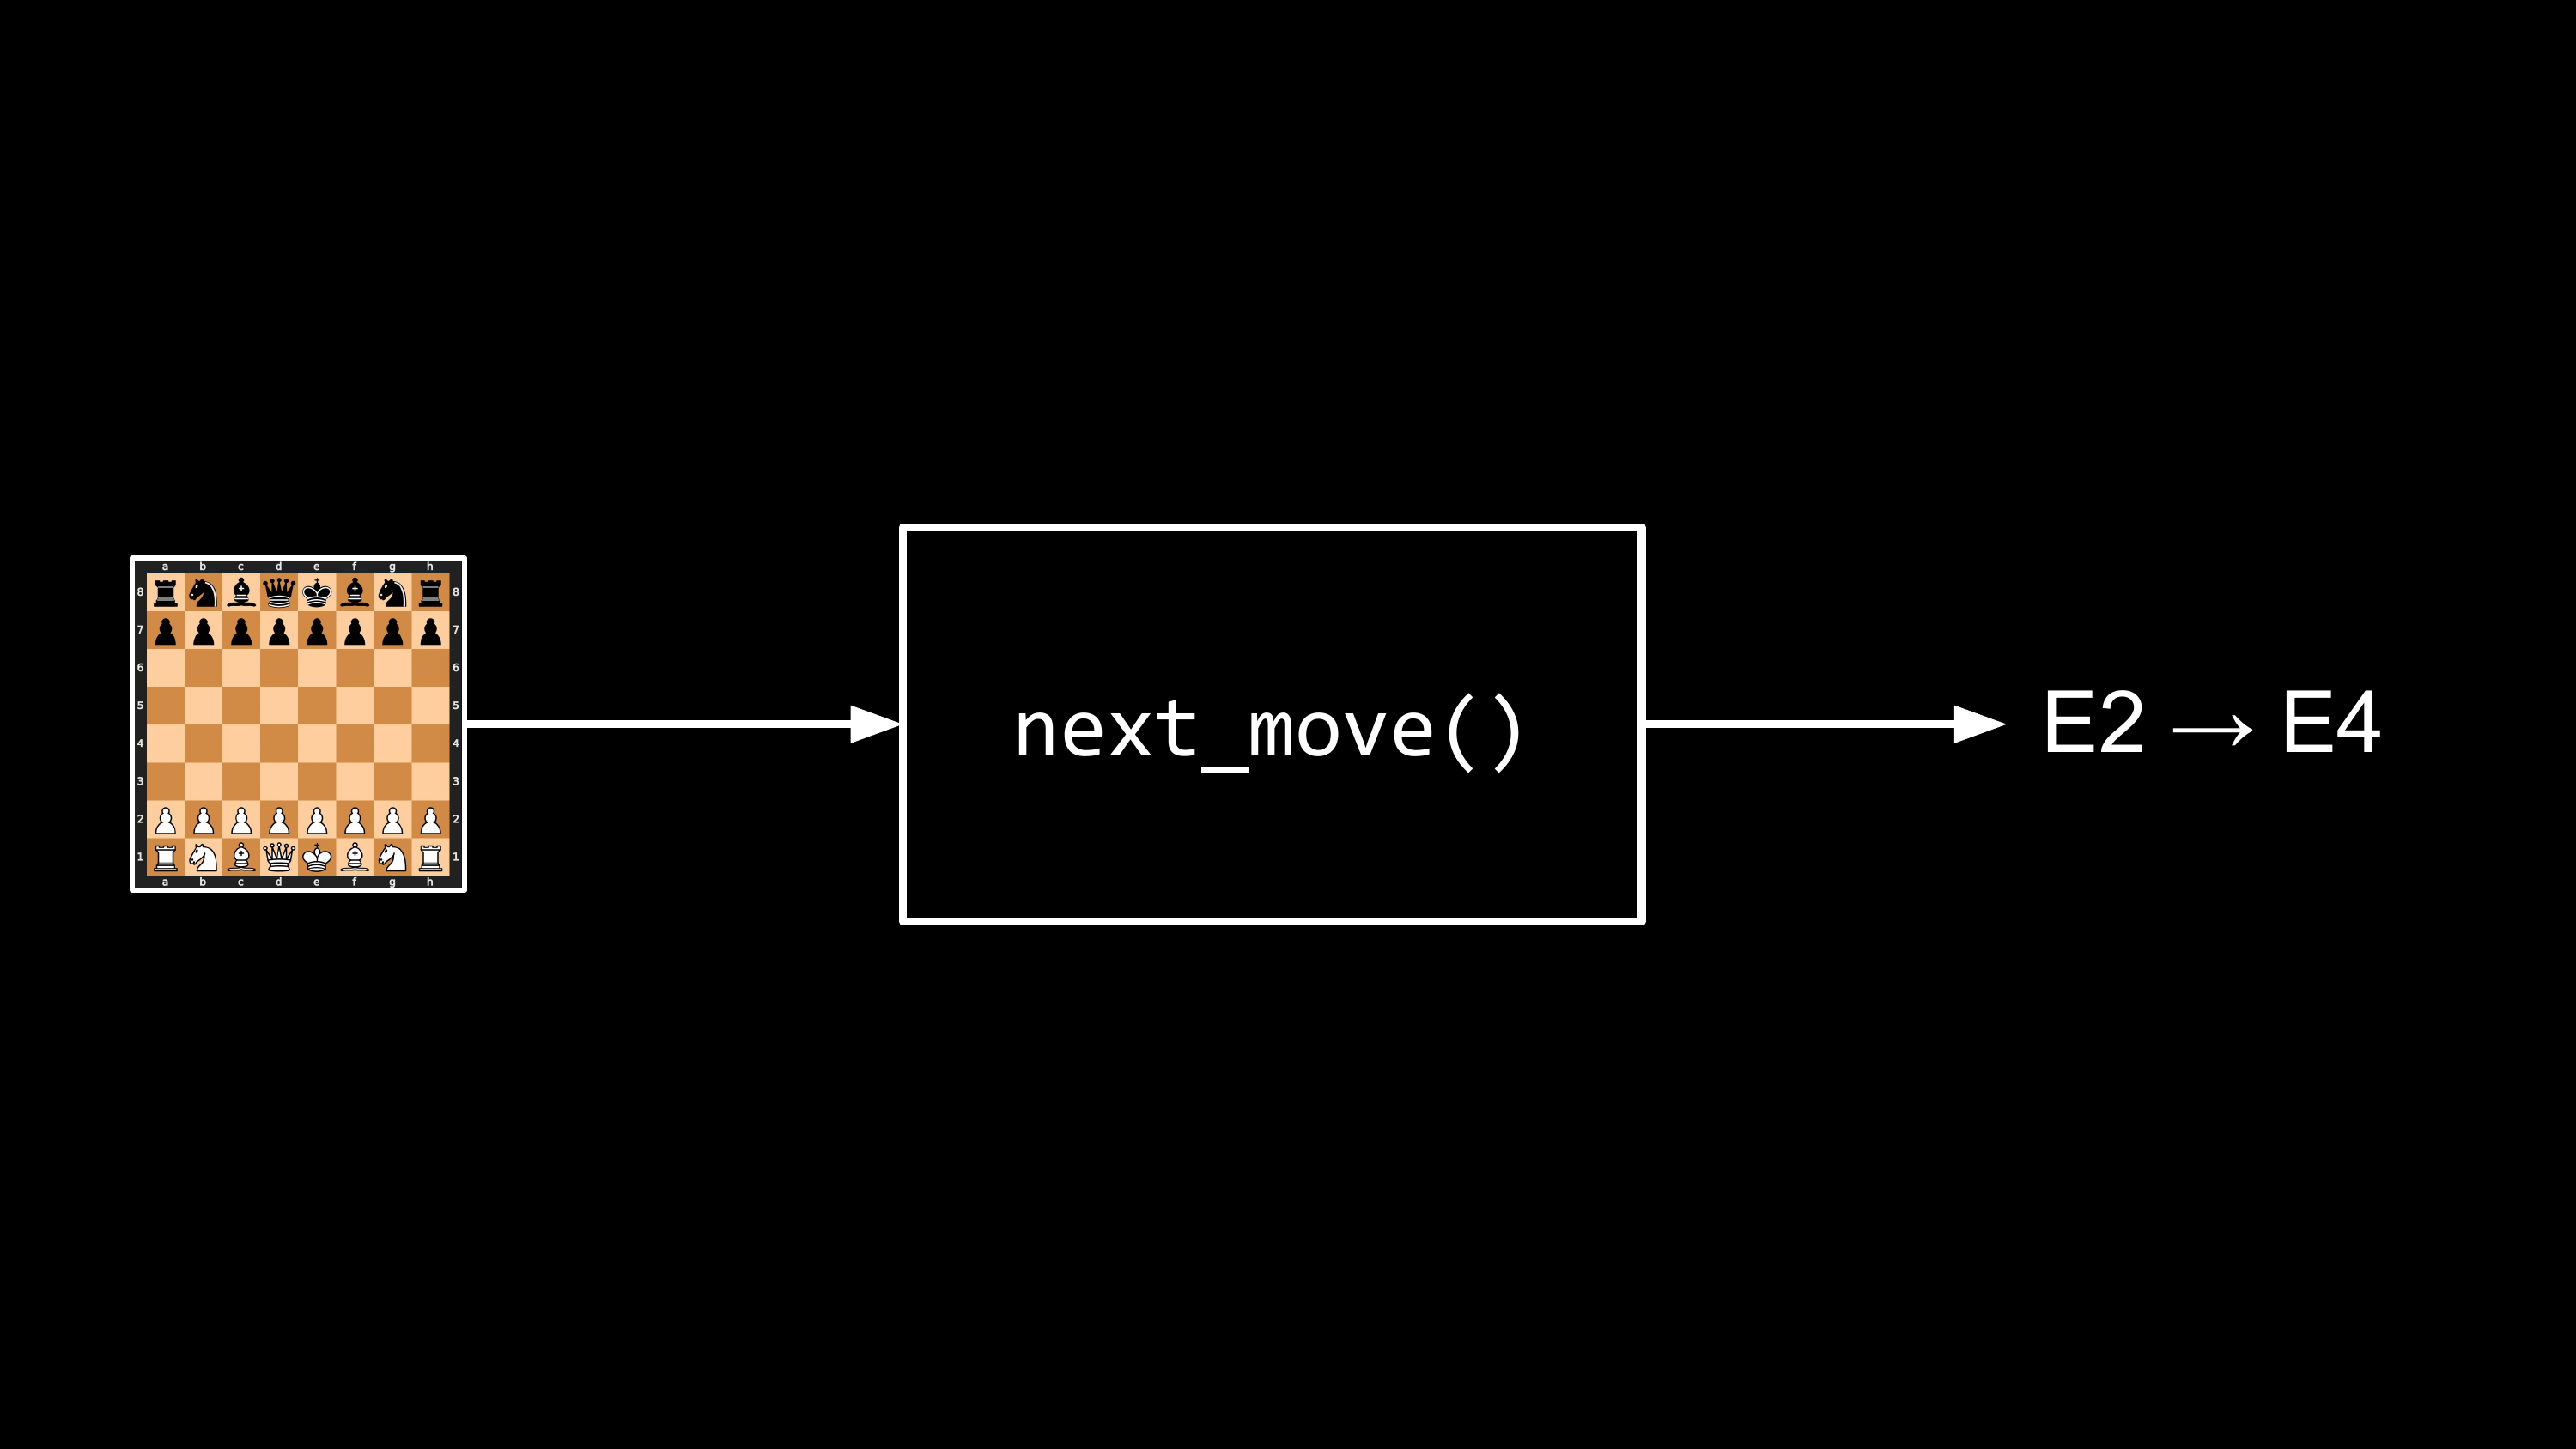
\includegraphics[width=1\linewidth,height=\textheight,keepaspectratio]{problem-solving_files/mediabag/problem_solving_exam1234.png}
\end{center}

Betrachten wir zunächst die Eingabe für dieses Problem: Wir können dem
Computer nicht einfach ein physisches Schachbrett zeigen, sondern müssen
überlegen, wie sich ein Schachbrett und die Position der Figuren in
digitaler Form darstellen lassen. Dabei kann es durchaus mehrere
Möglichkeiten geben, die uns ans Ziel führen.

Ein Schachbrett lässt sich etwa als Liste von 64 Feldern darstellen, die
von oben links nach unten rechts durchnummeriert sind. Für jedes Feld
speichern wir, ob es leer ist oder welche Figur darauf steht. Die
Figuren werden durch Buchstaben dargestellt -- zum Beispiel ``R'' für
den Turm (Englisch: Rook) oder ``N'' für den Springer (Englisch:
Knight). Für die Farben Schwarz und Weiß verwenden wir einfach 0 und 1.
Diese Darstellungsform reduziert unser Problem auf Listen, Zahlen und
Buchstaben in digitaler Form. Für Computer ist das eine leicht zu
verarbeitende Struktur, wie wir später noch sehen werden. Ein Beispiel
für eine solche Kodierung zeigt
Abbildung~\ref{fig-coding-chess-figures}.

\begin{figure}

\centering{

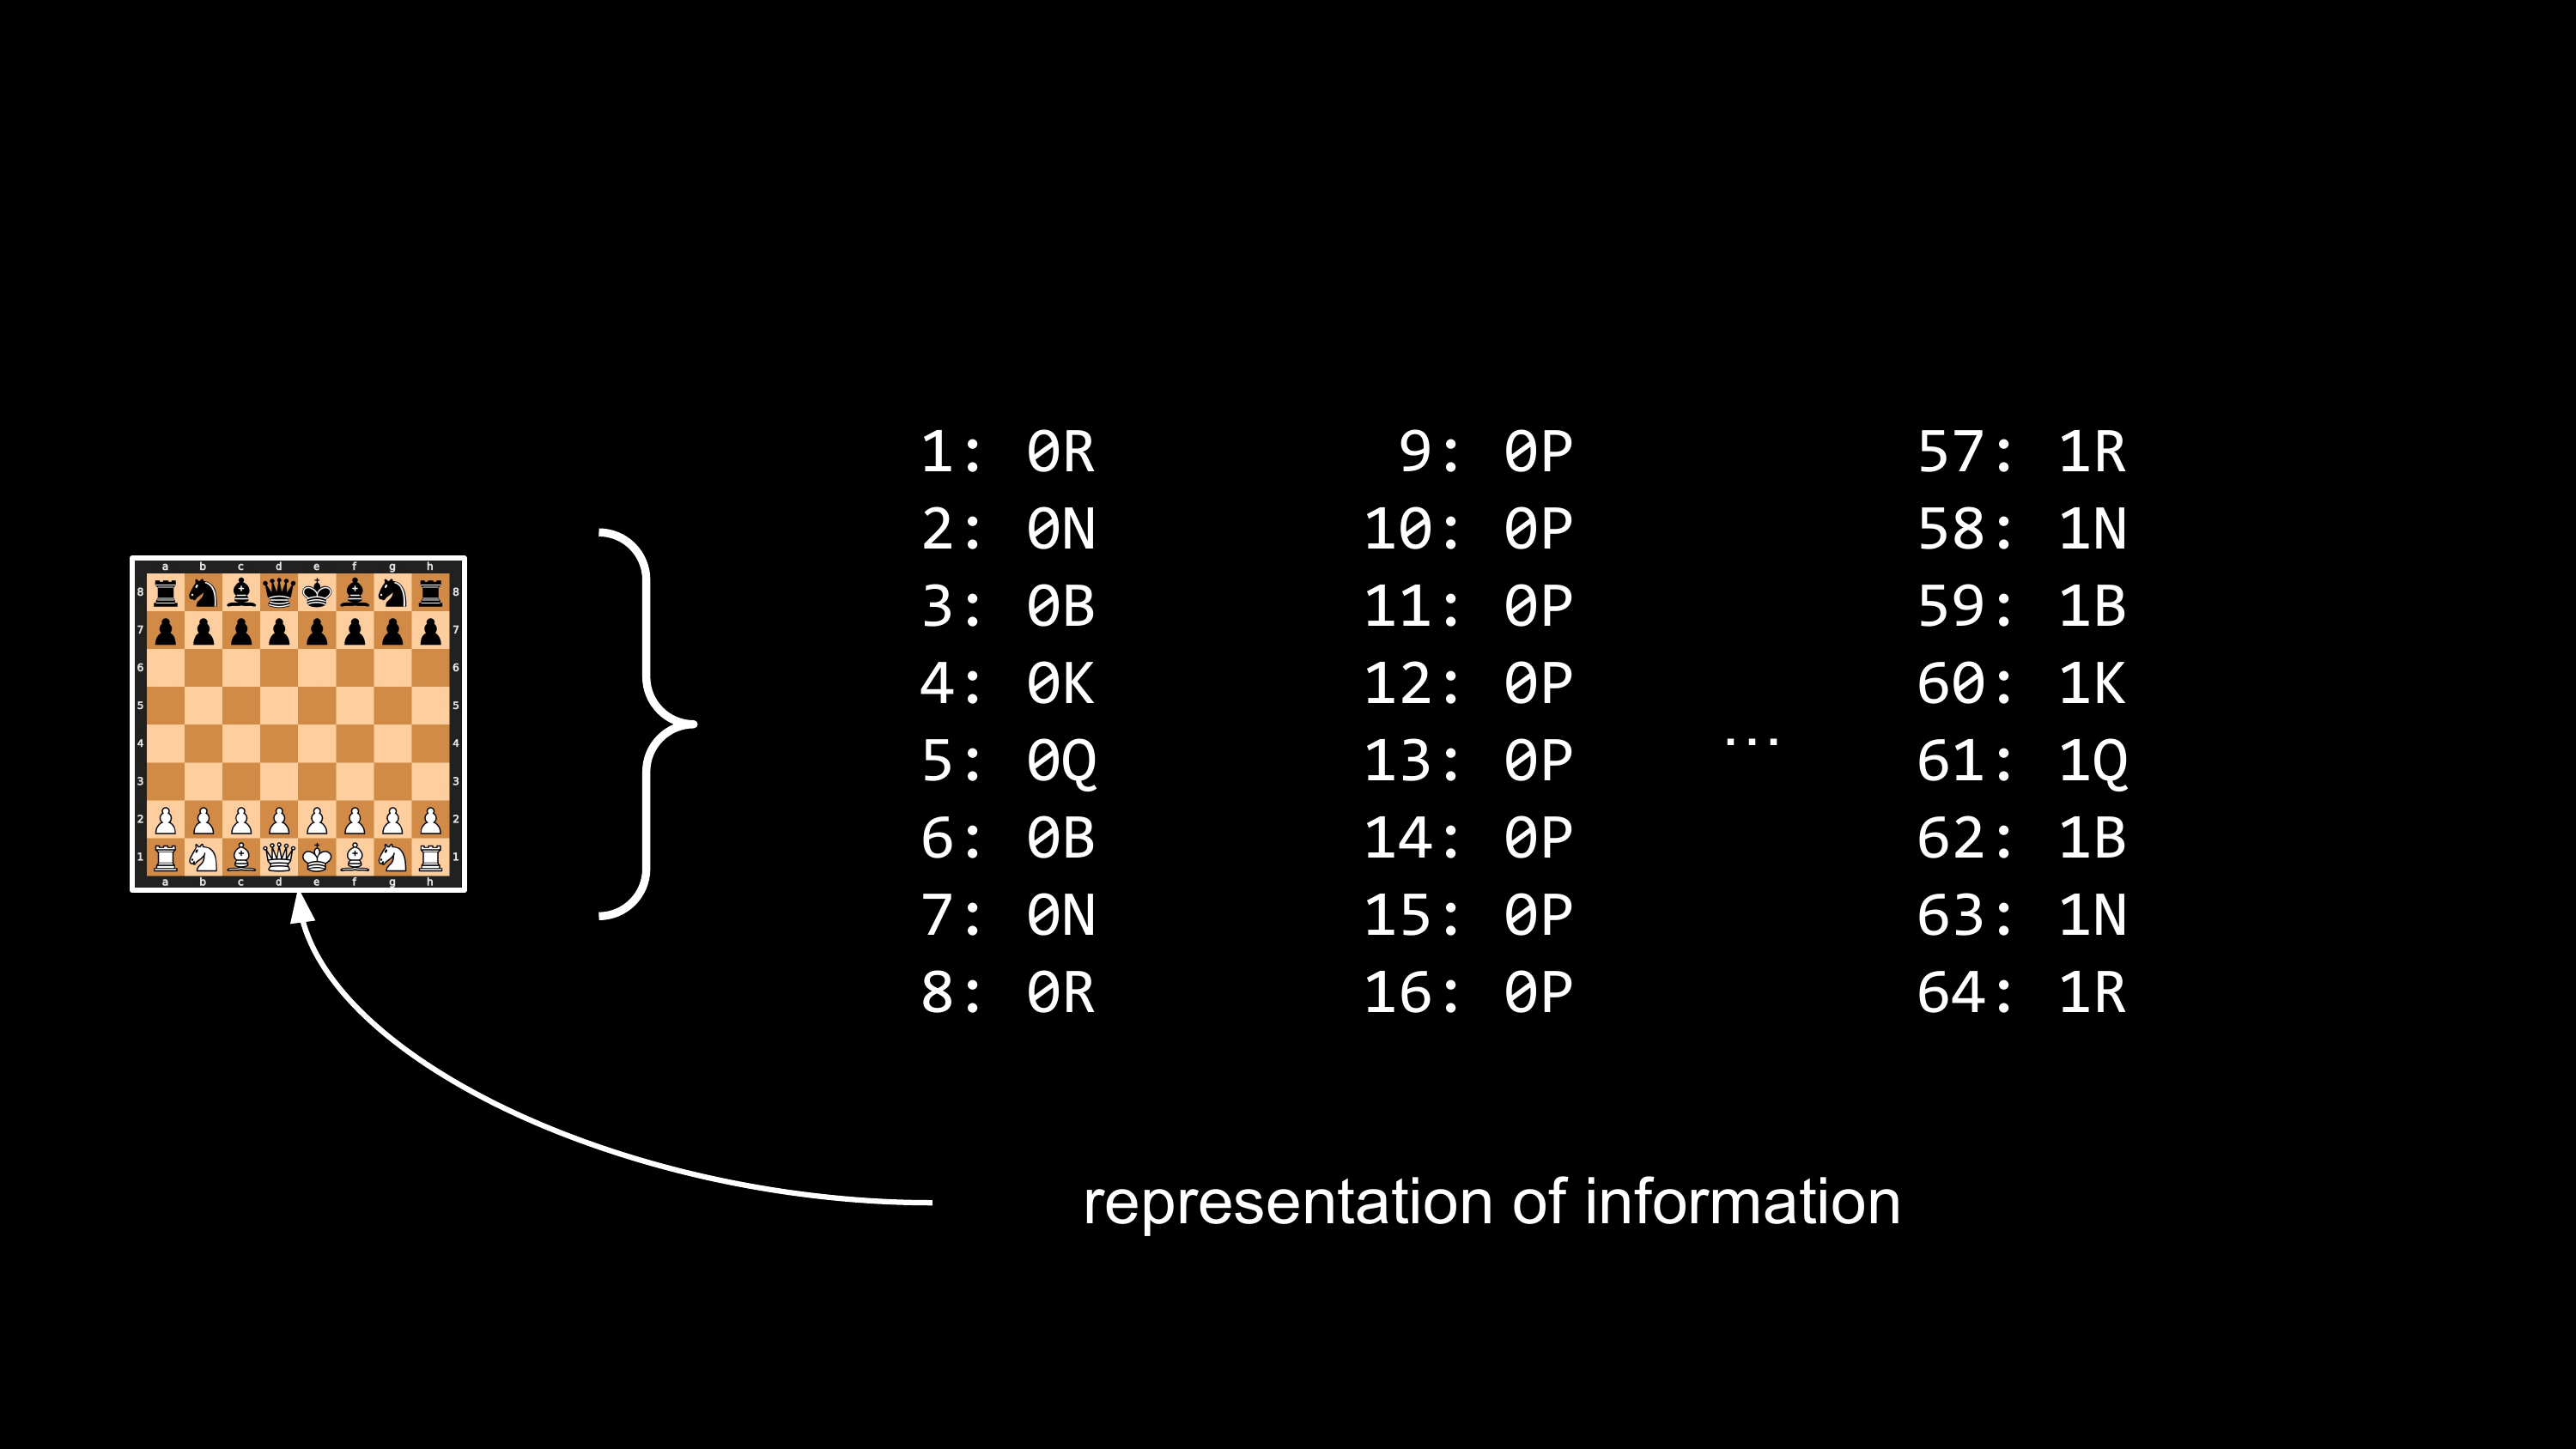
\includegraphics[width=1\linewidth,height=\textheight,keepaspectratio]{problem-solving_files/mediabag/problem_solving_exam12345.png}

}

\caption{\label{fig-coding-chess-figures}Beispiel für die Darstellung
von Schachfiguren als Zahlen und Buchstaben.}

\end{figure}%

Die Ausgabe, also der nächste Zug, lässt sich ebenfalls durch Zahlen und
Buchstaben darstellen. Eine weit verbreitete Notation gibt zunächst die
Koordinate des Ausgangsfelds an, von dem eine Figur gezogen werden soll,
gefolgt von der Koordinate des Zielfelds. Ein Beispiel wäre der Zug von
``E2 nach E4''. Statt ``E2'' und ``E4'' könnten wir ebenso die
entsprechende Zahl zwischen 1 und 64 aus unserer Liste verwenden, um mit
dem obigen Schema konsistent zu bleiben. Der Zug hieße dann ``53 nach
37''.

\subsubsection{Beispiel: Mit Computern
chatten}\label{beispiel-mit-computern-chatten}

Als drittes Beispiel betrachten wir die Verwendung von Chatprogrammen
wie ChatGPT. Seit seiner Veröffentlichung im November 2022 hat es die
Welt stark verändert und einen regelrechten KI-Hype ausgelöst. Ein
großes Sprachmodell wie GPT-4, das hinter dem heutigen ChatGPT steckt,
ist eine komplexe Software, die wir in diesem Buch nicht vollständig
ergründen können. Das Schöne an Modellen wie dem EVA-Modell ist jedoch,
dass sie komplexe Sachverhalte vereinfachen können -- so auch bei
Sprachmodellen. Das Problem, das Sprachmodelle lösen, lässt sich wie
alle Probleme in unserem EVA-Modell einfach darstellen.

\begin{figure}

\centering{

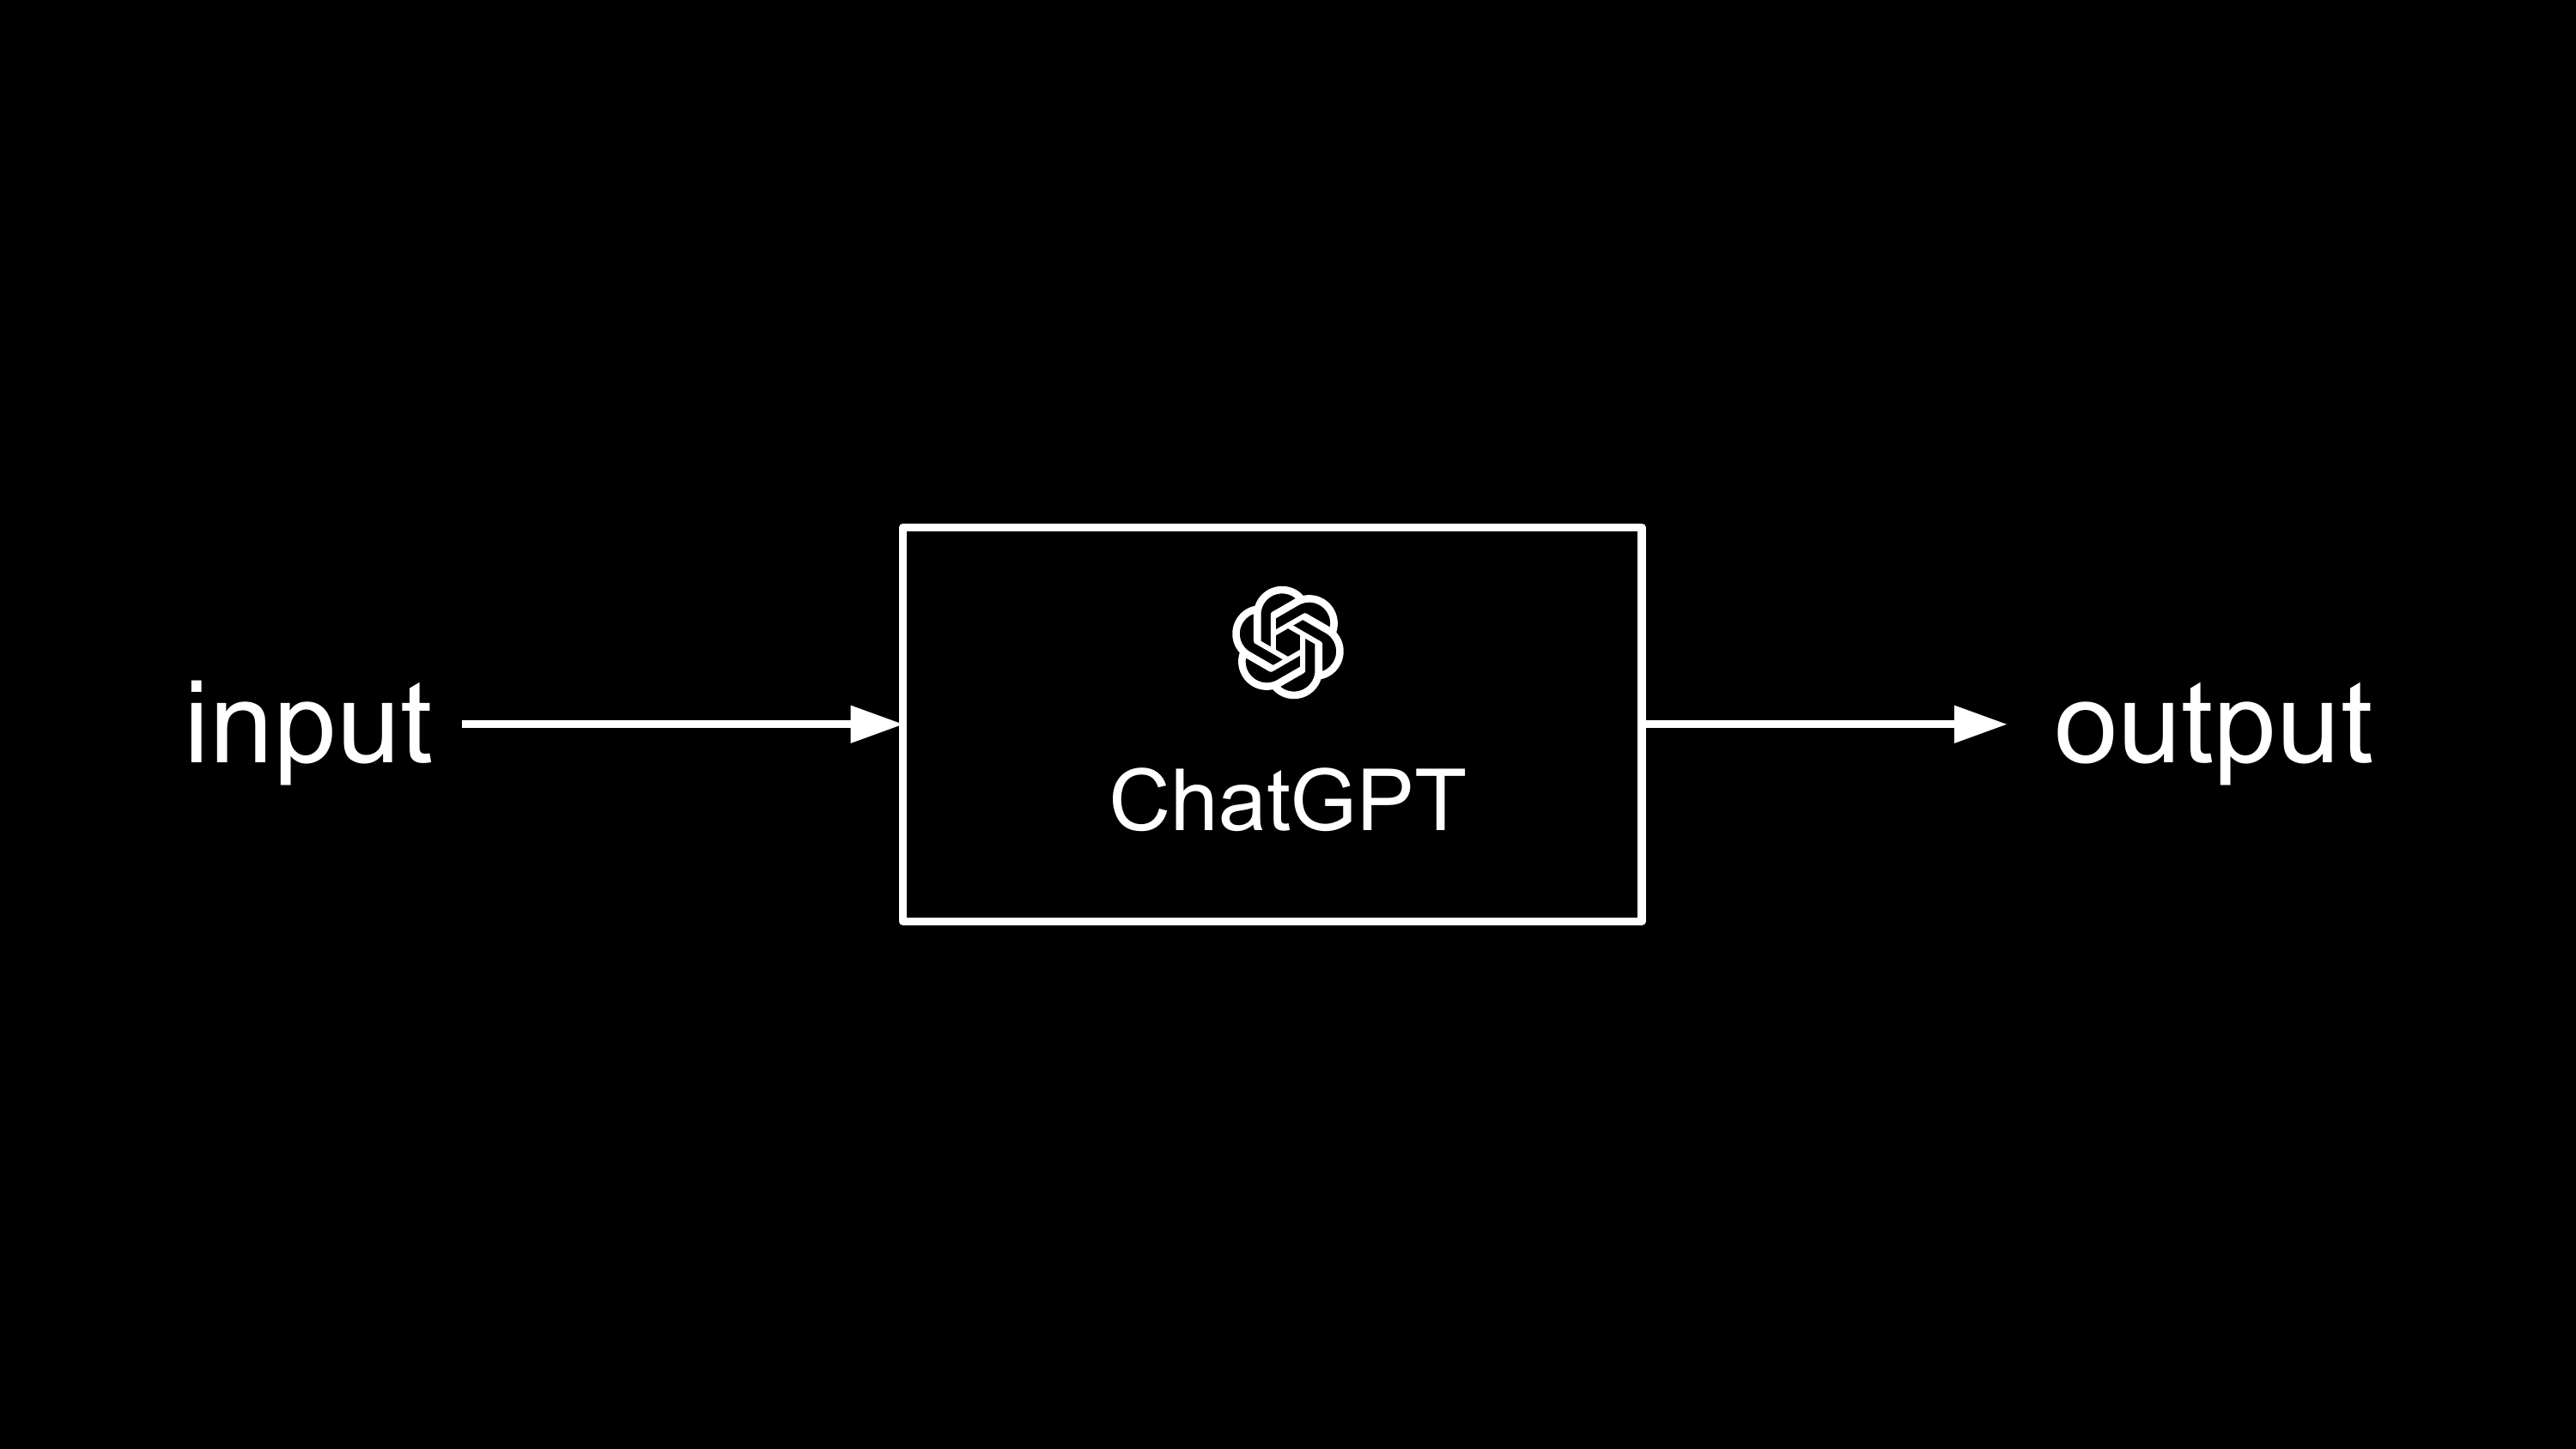
\includegraphics[width=1\linewidth,height=\textheight,keepaspectratio]{problem-solving_files/mediabag/problem_solving_exam123456.png}

}

\caption{\label{fig-eva-model-example-chatgpt}ChatGPT im EVA-Modell.}

\end{figure}%

Dabei betrachten wir das Sprachmodell -- oder ChatGPT -- als Blackbox,
ohne die internen Prozesse genauer zu definieren. Für unser Modell
genügt es zu verstehen, dass wir eine Eingabe in Form einer Nachricht an
ChatGPT benötigen und als Ausgabe eine Antwort erhalten. Auch hier
stellt sich die Frage, wie wir beides digital repräsentieren können,
damit ChatGPT damit arbeiten kann.

Klassischerweise bestehen sowohl Eingabe als auch Ausgabe einfach aus
Texten -- allerdings beherrschen moderne Sprachmodelle auch andere
Eingabeformen wie Bilder oder gesprochene Sprache über ein Mikrofon. Wir
sprechen dann von multimodalen KI-Modellen. Bei Bildern stehen wir vor
demselben Repräsentationsproblem wie bei unserer Drohnenaufnahme. Bei
der Sprache stellt sich neben der Repräsentation von Audioinhalten die
Frage, wie wir gesprochene Worte überhaupt in eine digitale Form
überführen können. Auch dazu erfahren wir im späteren Verlauf des Buches
mehr.

\subsection{Die Lösung des Problems}\label{die-luxf6sung-des-problems}

Anhand des EVA-Modells wird deutlich, dass wir dem Computer
Informationen in Form von digitalen Daten bereitstellen müssen, mit
denen er arbeiten kann. Was aber genau soll er damit machen? Hier kommt
der mittlere Kasten des Modells ins Spiel -- die eigentliche Lösung des
Problems.

\begin{center}
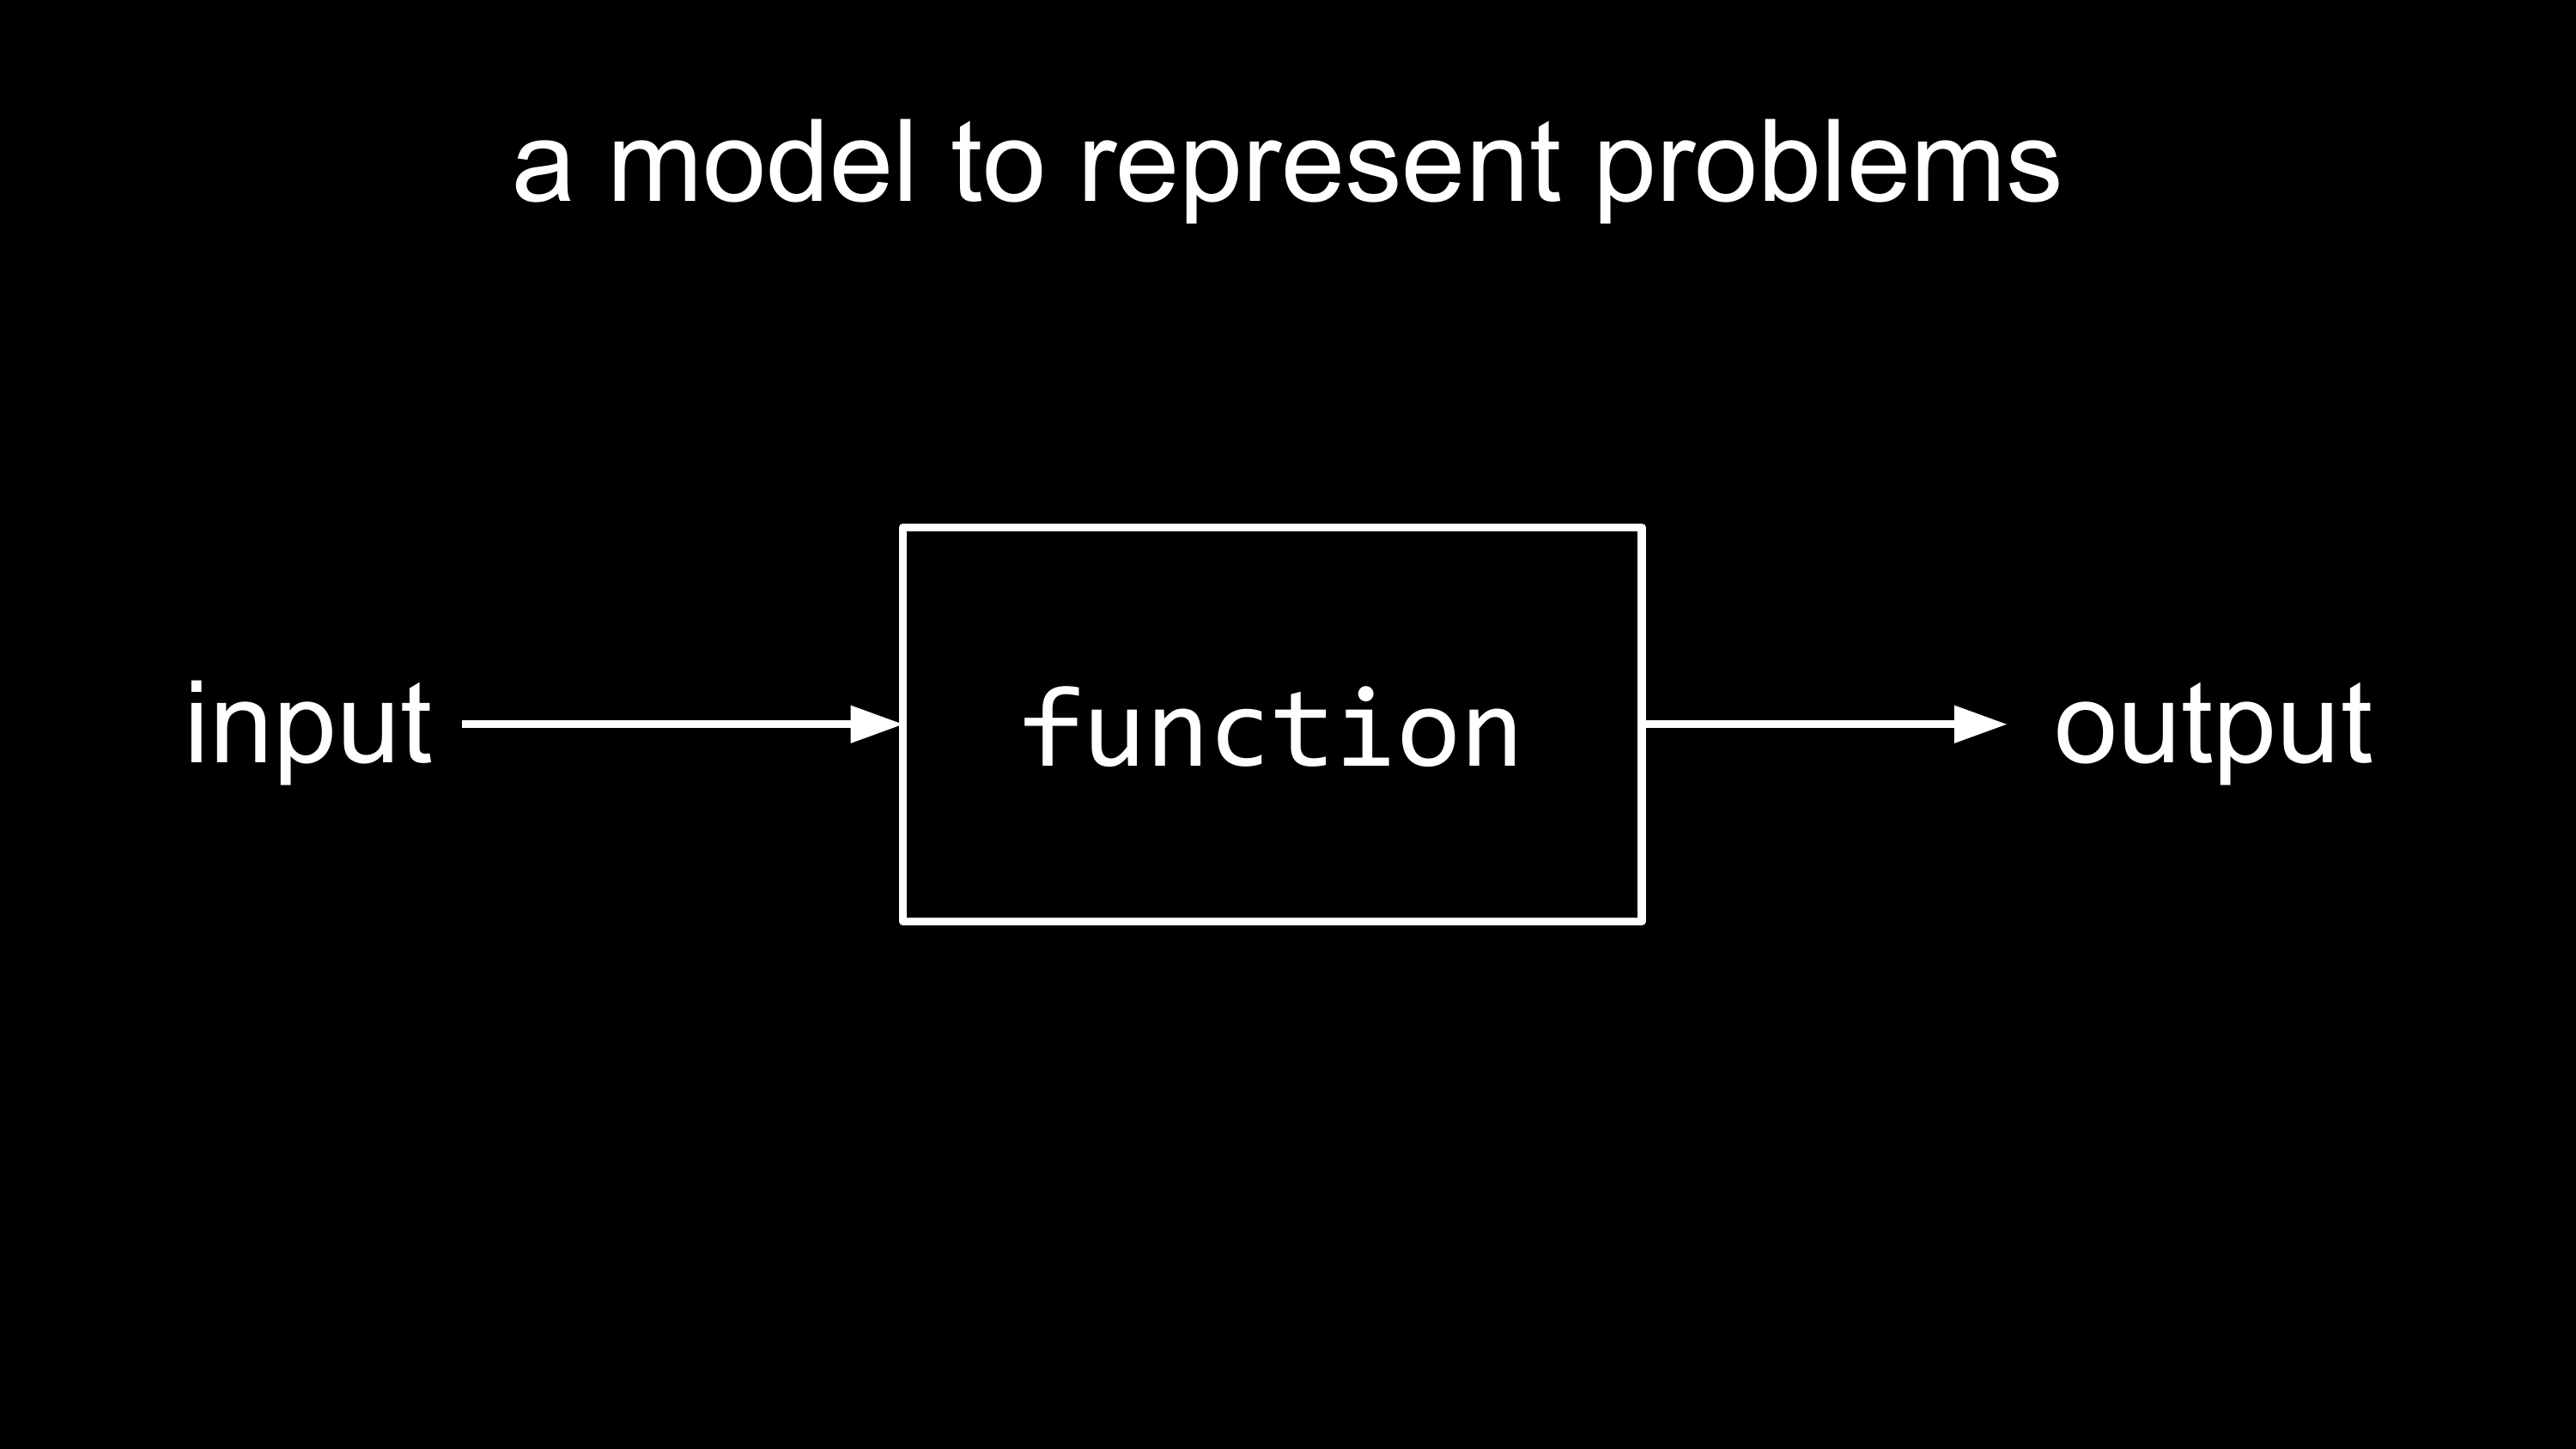
\includegraphics[width=1\linewidth,height=\textheight,keepaspectratio]{problem-solving_files/mediabag/problem_solving_inpu12.png}
\end{center}

In der Informatik nennen wir die Beschreibung zur Lösung eines Problems
einen \textbf{Algorithmus}. Ein Algorithmus ist eine
Schritt-für-Schritt-Anleitung zur Problemlösung und ist zunächst
unabhängig von Computern. Das bedeutet, wir können die Lösung eines
Problems ohne Bezug zu einem Computer beschreiben und nennen das einen
Algorithmus.

Stellt euch dazu zum Beispiel eine IKEA-Aufbauanleitung vor. Sie
beschreibt in sequenziellen Schritten, was zu tun ist, um das fertige
Möbelstück zu bekommen. Die Eingabe besteht aus den mitgelieferten
Teilen, Schrauben und dem benötigten Werkzeug für den Zusammenbau. Die
Ausgabe ist das fertige Regal (oder ein anderes Möbelstück) -- und das
alles ganz ohne Computer.

Oder nehmt das Kochrezept eure Lieblingsessens. Auch ein Kochrezept ist
ein Algorithmus: Die Eingabe besteht aus den Zutaten und
Küchenutensilien, die Verarbeitung erfolgt durch die
Schritt-für-Schritt-Anleitung, und die Ausgabe ist das fertige Gericht.
Wie bei der IKEA-Anleitung ist der Algorithmus unabhängig von einem
Computer -- er beschreibt lediglich die Lösung des Problems ``Wie koche
ich dieses Gericht?''.

Zu Beginn des Kapitels haben wir festgestellt, dass Computer aufgrund
ihrer Geschwindigkeit und Fehlerfreiheit besonders gut zur Problemlösung
geeignet sind -- insbesondere bei häufig wiederkehrenden Problemen. Die
beiden genannten Beispiele, das IKEA-Regal und das Kochrezept, eignen
sich allerdings nicht für eine direkte Umsetzung durch Computer. Der
Grund liegt in den analogen Eingaben (Baumaterial, Kochzutaten) und
Ausgaben (Möbelstück, fertige Mahlzeit). Diese kann ein Computer nicht
unmittelbar verarbeiten. Dafür wären Roboter nötig, die mit der
physischen Welt interagieren können. Eine solche Automatisierung lohnt
sich heute nur bei Aufgaben, die sehr häufig auftreten und ansonsten mit
hohen Kosten verbunden sind -- wie etwa in der Automobilindustrie, wo
computergesteuerte Roboter in der Produktion zum Einsatz kommen.

Nehmen wir an, dass Haushaltsroboter in Zukunft erschwinglich werden und
uns beim Kochen unseres Lieblingsgerichts helfen können. Wie vermitteln
wir dann dem Roboter -- im Grunde ein Computer mit Armen und Beinen --
den Algorithmus für unser Rezept? Die Lösung liegt in der
Programmierung: Wir erstellen ein \textbf{Programm} in einer
computerverständlichen Sprache. Dieses Programm wandelt die Anweisungen
aus unserem Kochbuch in Befehle um, die der Computer verstehen und
ausführen kann. Genau genommen besteht ein Programm ebenfalls nur aus
Informationen, und wir müssen herausfinden, wie wir diese Informationen
digital darstellen können. Die Lösung besteht in der Verwendung einer
\textbf{Programmiersprache} wie Python, die wir später kennenlernen
werden.

\section{Welche Strategien helfen bei der Lösung von
Problemen?}\label{welche-strategien-helfen-bei-der-luxf6sung-von-problemen}

Die konkrete Lösung und der zugehörige Algorithmus sehen für jedes
Problem unterschiedlich aus. Das Erkennen von Pflanzen folgt einer
anderen Logik als die Entscheidung, welche Schachfigur als nächstes
gezogen werden soll. Dennoch gibt es universelle Lösungsstrategien, die
auf viele Probleme anwendbar sind, um sie möglichst effizient zu lösen.
Im Folgenden betrachten wir drei dieser Strategien.

\subsection{\texorpdfstring{Problemzerlegung (\emph{Problem
Decomposition})}{Problemzerlegung (Problem Decomposition)}}\label{problemzerlegung-problem-decomposition}

Eine universelle Strategie zur Lösung komplexer Probleme ist die
Zerlegung in kleinere Schritte oder Teilprobleme. Jedes dieser
Teilprobleme ist unterschiedlich und erfordert einen spezifischen
Lösungsansatz. Nehmen wir als Beispiel das Zählen von Pflanzen auf einer
Drohnenaufnahme. Dieses komplexe Problem lässt sich, ausgehend von der
Eingabe -- dem digitalen Bild -- in drei Teilprobleme zerlegen:

\begin{enumerate}
\def\labelenumi{\arabic{enumi}.}
\tightlist
\item
  Pflanzen auf dem Bild lokalisieren
\item
  Lokalisierte Pflanzen klassifizieren: Maispflanze oder nicht?
\item
  Identifizierte Maispflanzen zählen
\end{enumerate}

\begin{center}
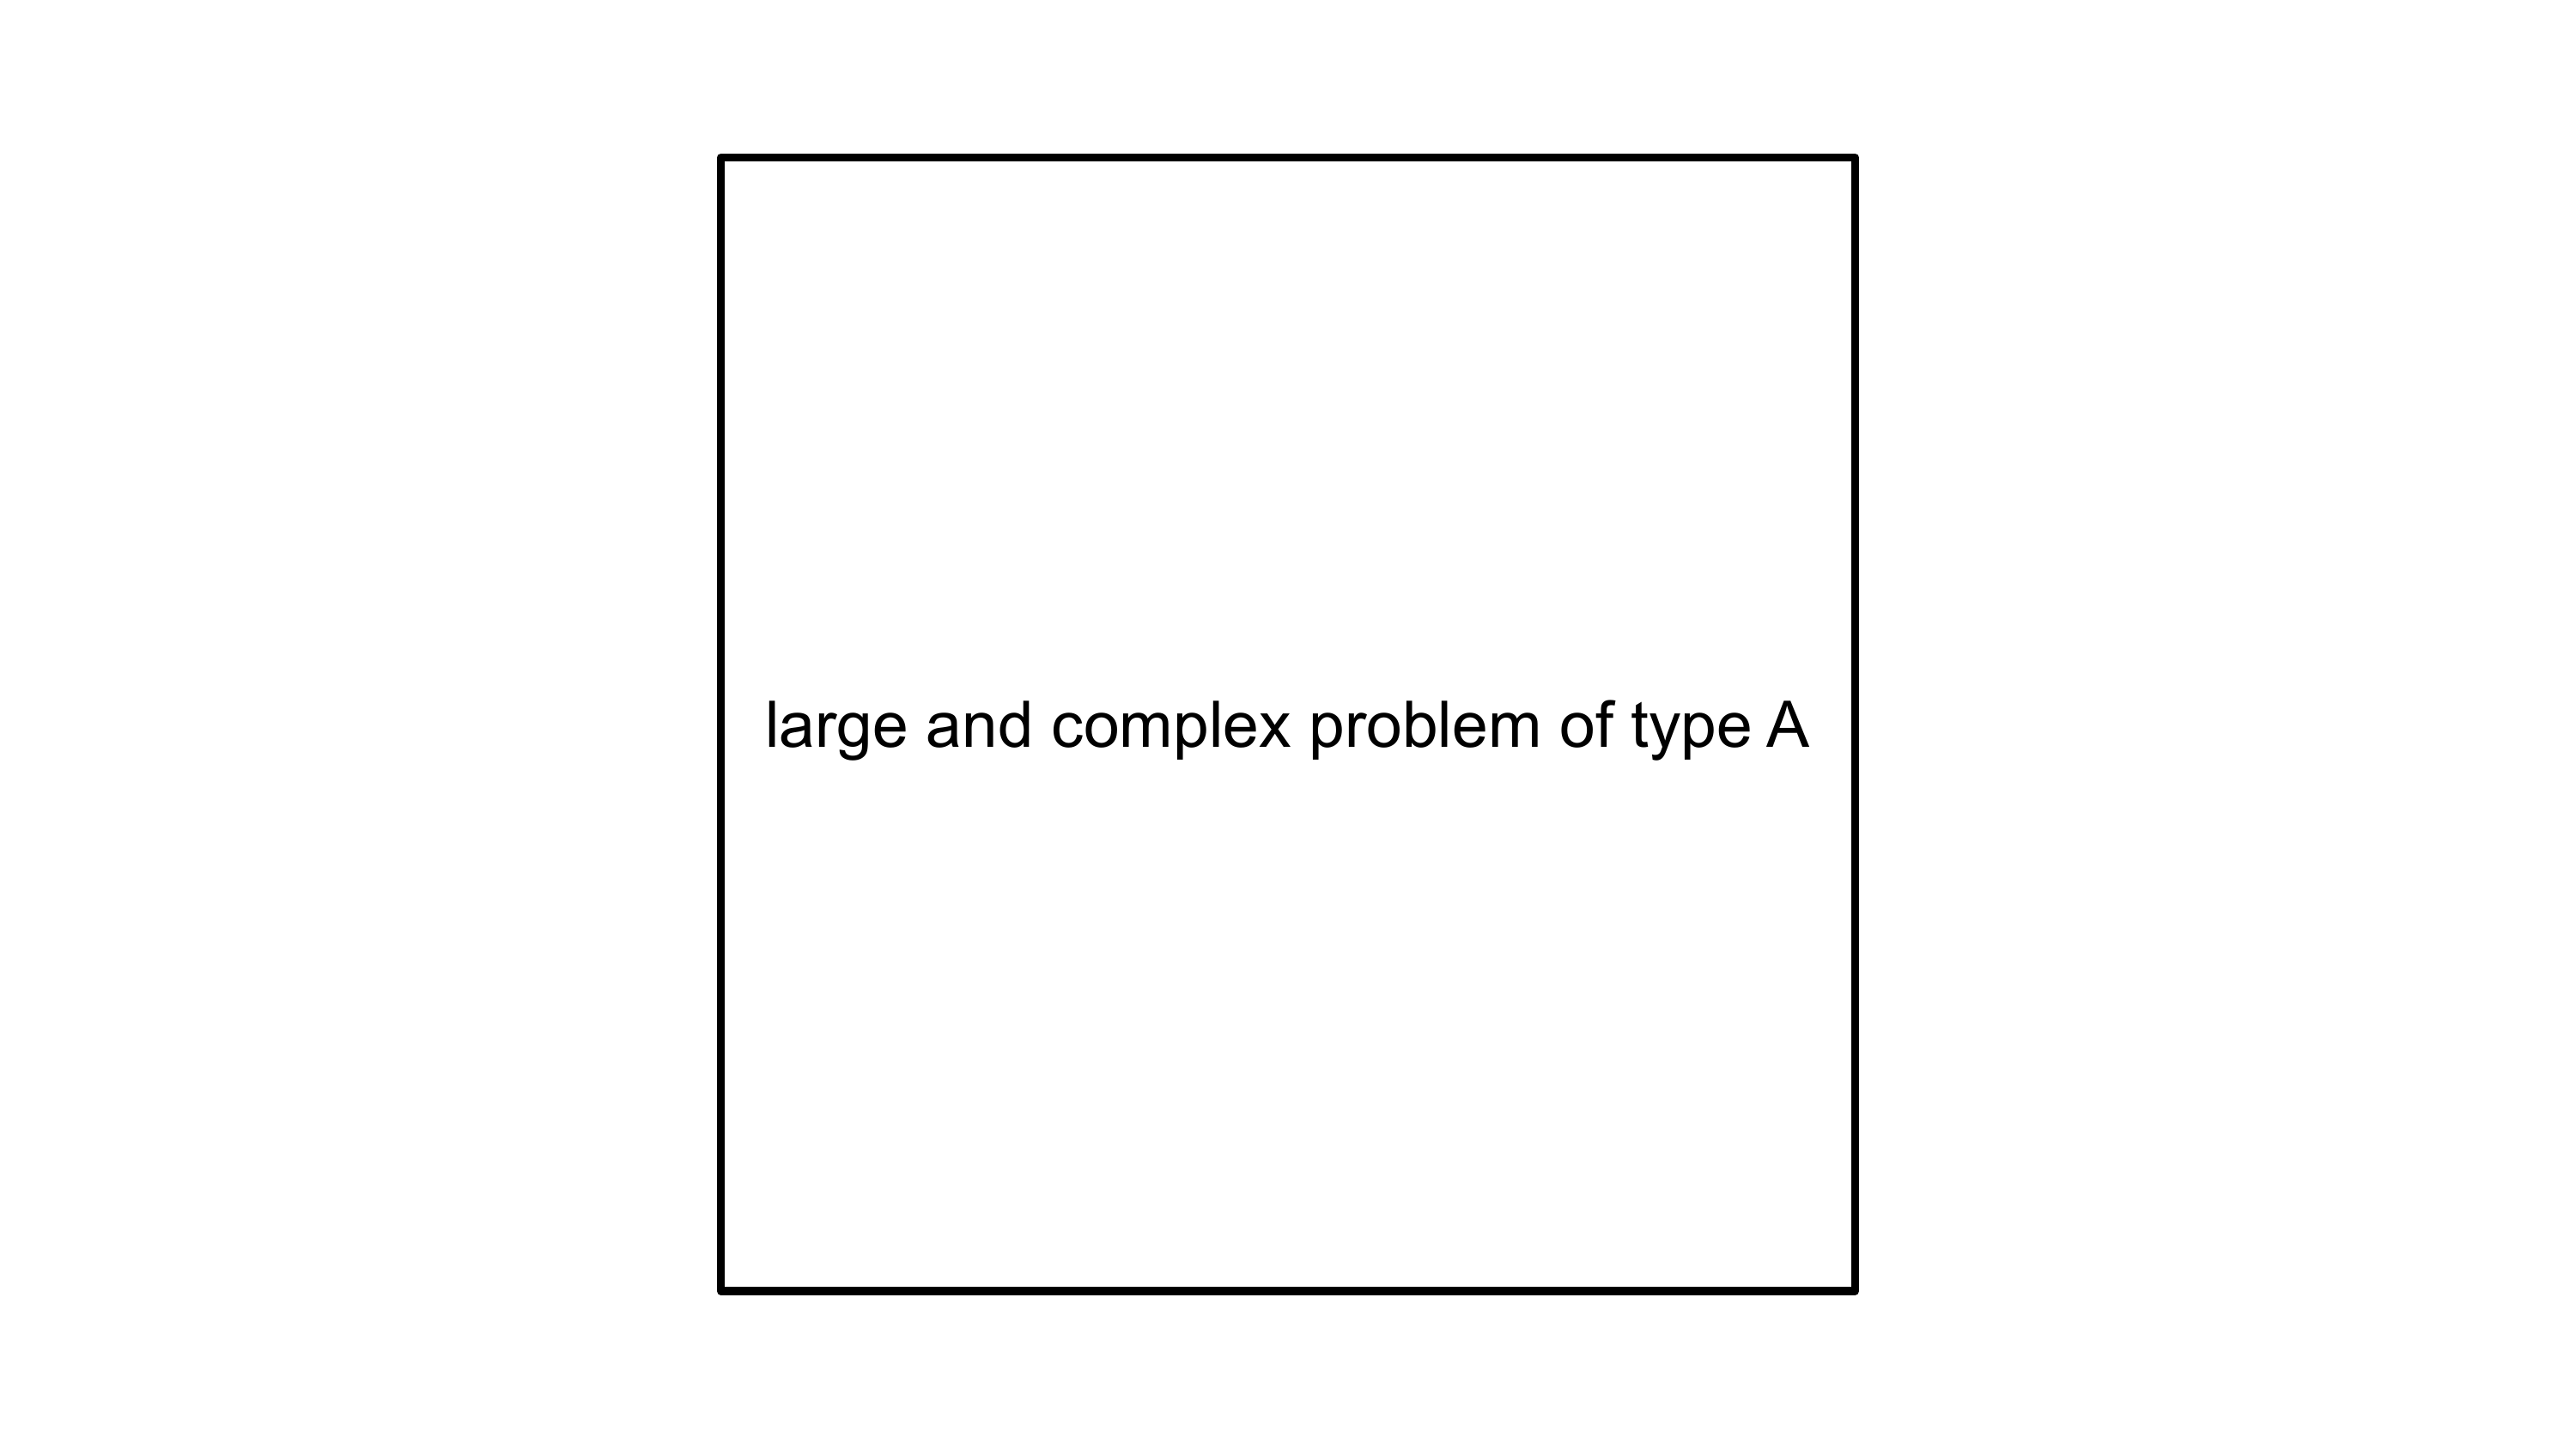
\includegraphics[width=1\linewidth,height=\textheight,keepaspectratio]{problem-solving_files/mediabag/problem_solving_larg.png}
\end{center}

Jedes dieser Teilprobleme erfordert einen eigenen Algorithmus. Dabei ist
es möglich, die Teilprobleme noch weiter zu zerlegen, um sie besser
bearbeiten zu können.

\begin{center}
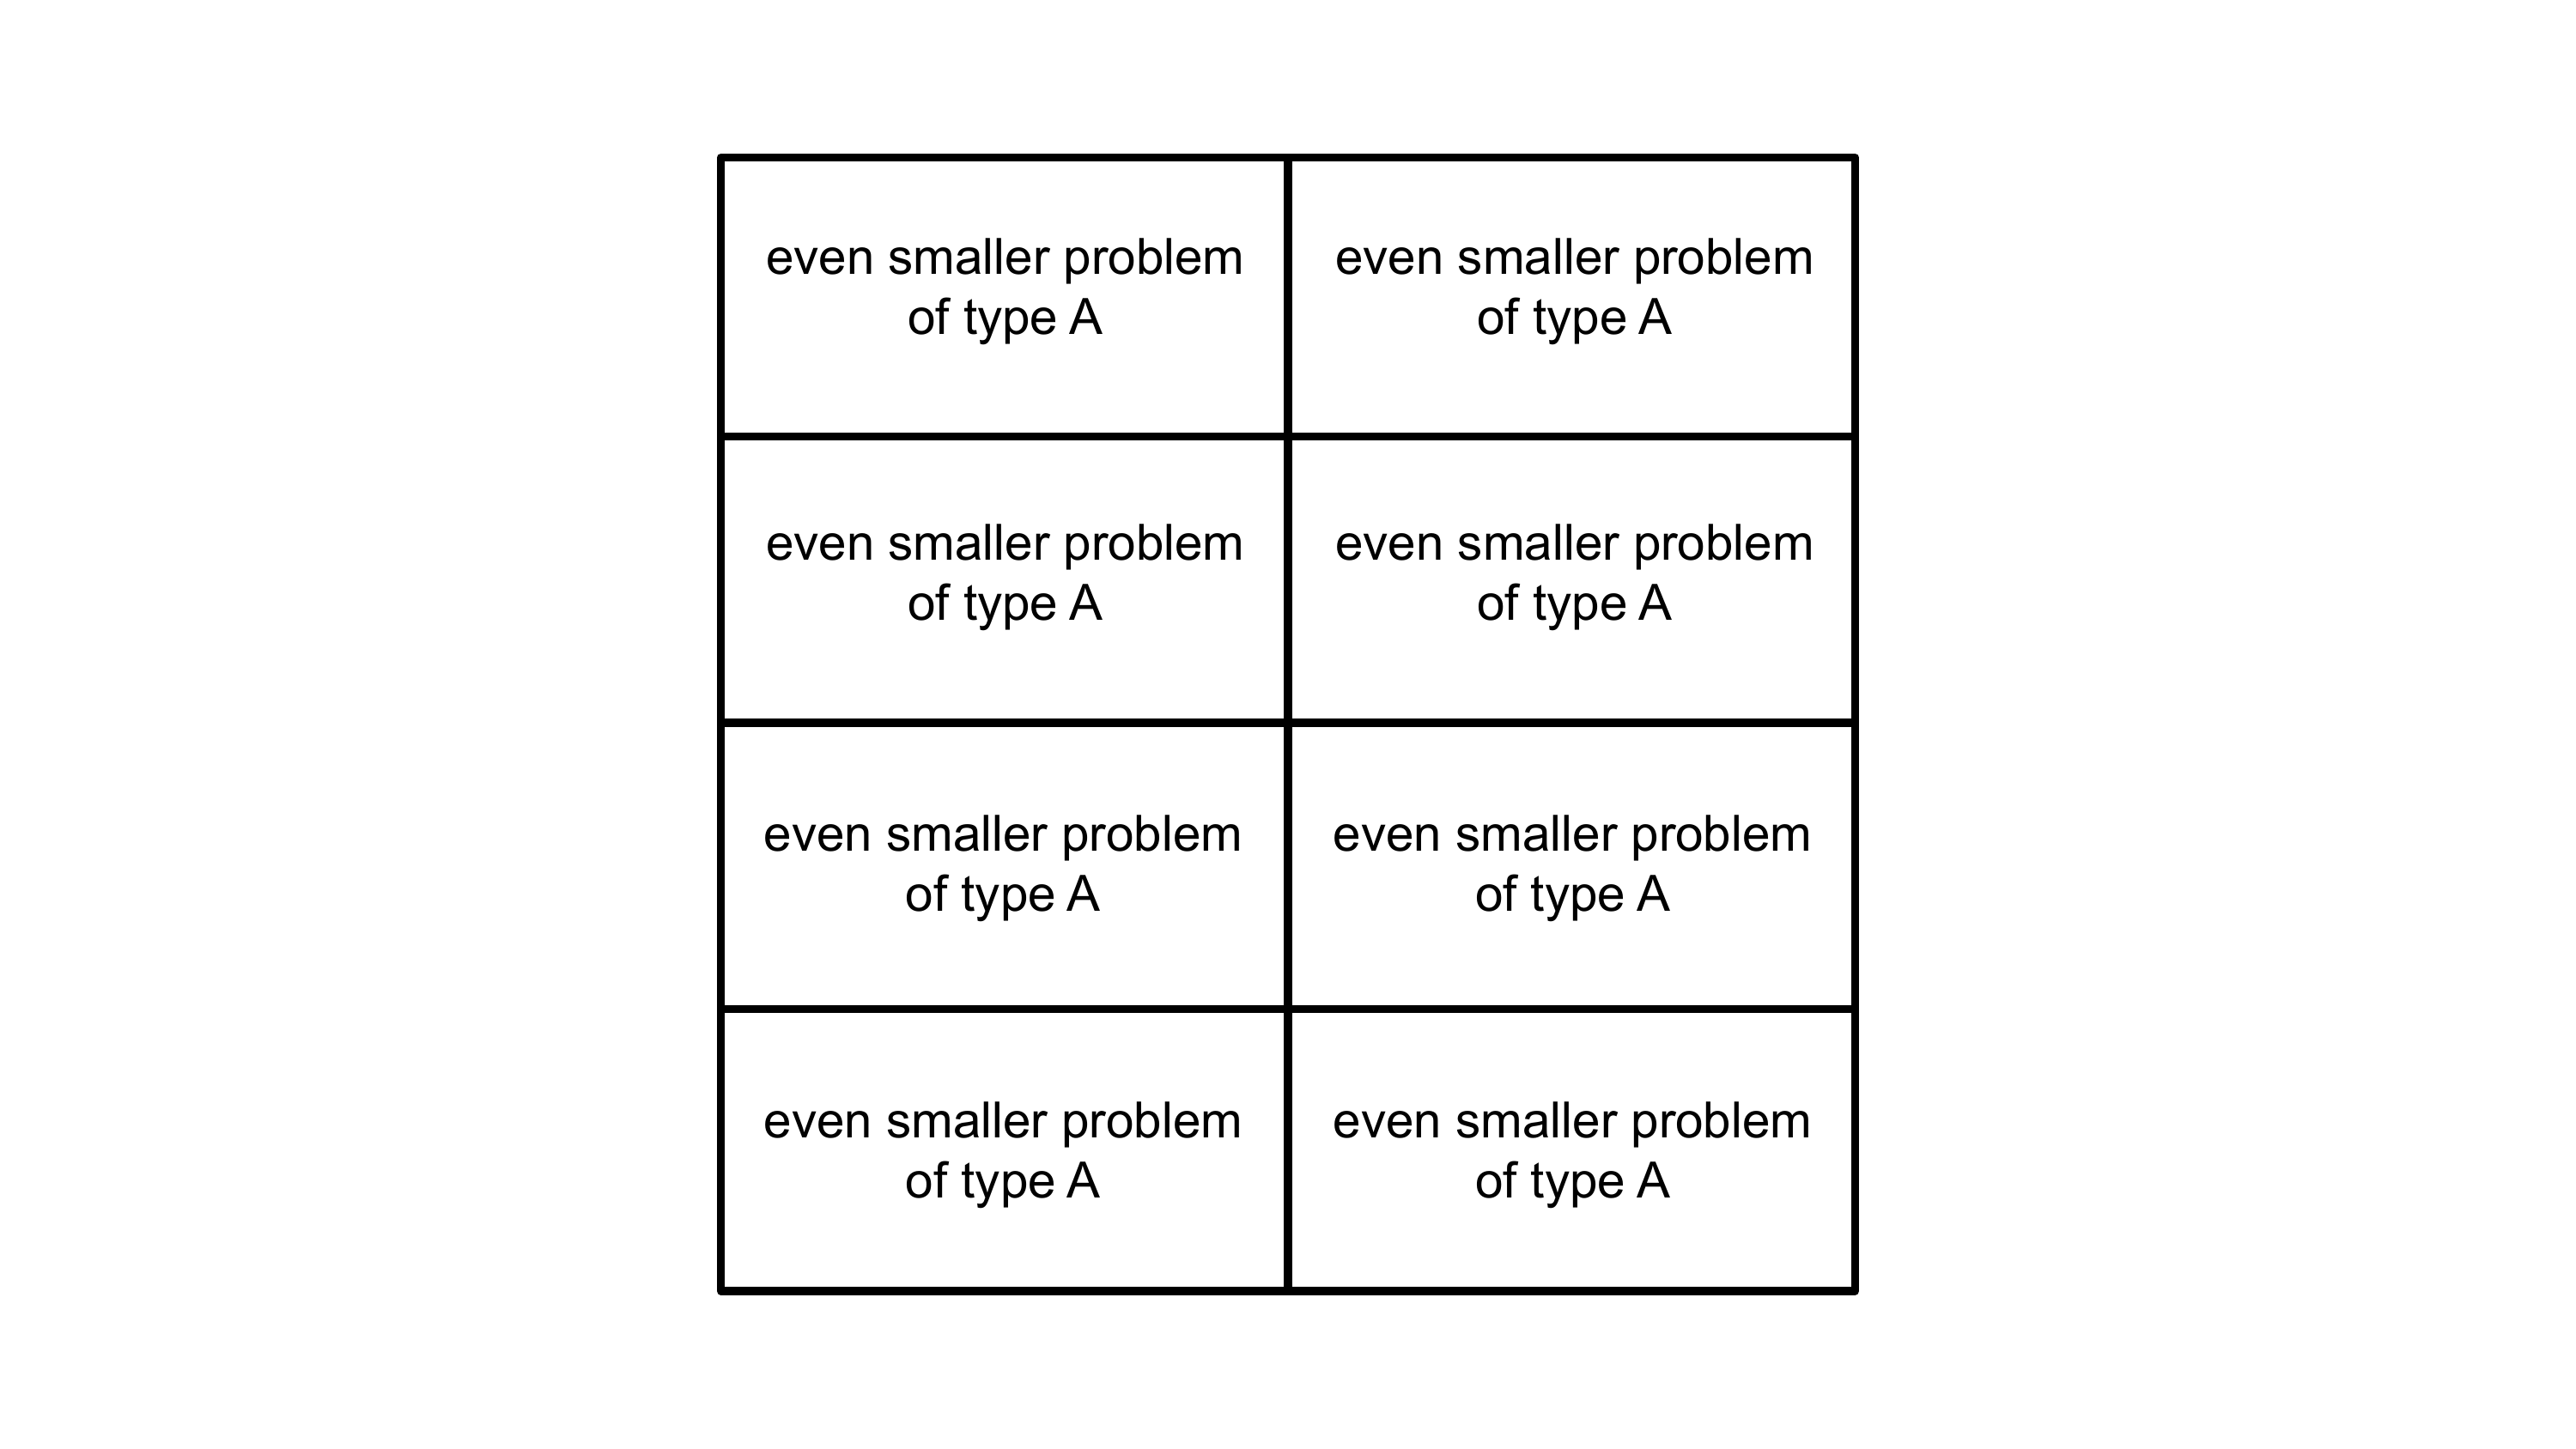
\includegraphics[width=1\linewidth,height=\textheight,keepaspectratio]{problem-solving_files/mediabag/problem_solving_even.png}
\end{center}

Die Identifizierung sinnvoller Teilprobleme erfordert ein ausgeprägtes
analytisches Denkvermögen. Dies ist besonders wichtig im Umgang mit
Computern. Wie wir beim Erlernen der Programmierung sehen werden, ist
die Zerlegung eines Problems in kleine, lösbare Schritte der Schlüssel
zur Beherrschung seiner Komplexität.

\subsection{\texorpdfstring{Teile und Herrsche (\emph{Divide and
Conquer})}{Teile und Herrsche (Divide and Conquer)}}\label{sec-divide-and-conquer}

Die ``Teile und Herrsche''-Strategie ist ein Ansatz zur Lösung komplexer
Probleme, bei dem wir das Hauptproblem schrittweise in immer kleinere
Teilprobleme zerlegen, bis diese einfach zu lösen sind. Dabei gehen wir
rekursiv vor: Wir teilen das ursprüngliche Problem in kleinere Teile,
diese kleineren Probleme wiederum in noch kleinere Teile und so weiter.
Die Rekursion endet, wenn die Probleme so klein sind, dass sie sich
nicht weiter aufteilen lassen und die Lösung direkt ersichtlich ist.

Anders als bei der Problemzerlegung sind die Teilprobleme beim Divide
and Conquer-Ansatz dadurch gleichartig und stellen nur kleinere
Instanzen des ursprünglichen Problems dar. Die einzelnen Lösungen für
jedes Teilproblem werden dann schrittweise wieder zusammengeführt, um
die Gesamtlösung zu erhalten. Ein klassisches Beispiel ist die
Sortierung einer langen Liste von Zahlen: Wir teilen die Liste immer
wieder in der Mitte, bis nur noch einzelne Zahlen übrig sind, und fügen
diese dann in sortierter Reihenfolge wieder zusammen.

Ein anderes Beispiel ist die binäre Suche in einer sortierten Liste.
Hier betrachten wir das Element in der Mitte der Liste und vergleichen
es mit dem gesuchten Element. Da die Liste sortiert ist, können wir
entscheiden, in welchem Teil der Liste wir weitersuchen müssen. Im
zweiten Schritt suchen wir nur in diesem Teil weiter und haben damit das
Problem halbiert. Die Natur des Problems bleibt dabei gleich, und wir
können erneut genauso verfahren -- so lange, bis wir nur noch ein
Element übrig haben, das entweder das gesuchte Element ist oder nicht.

\begin{center}
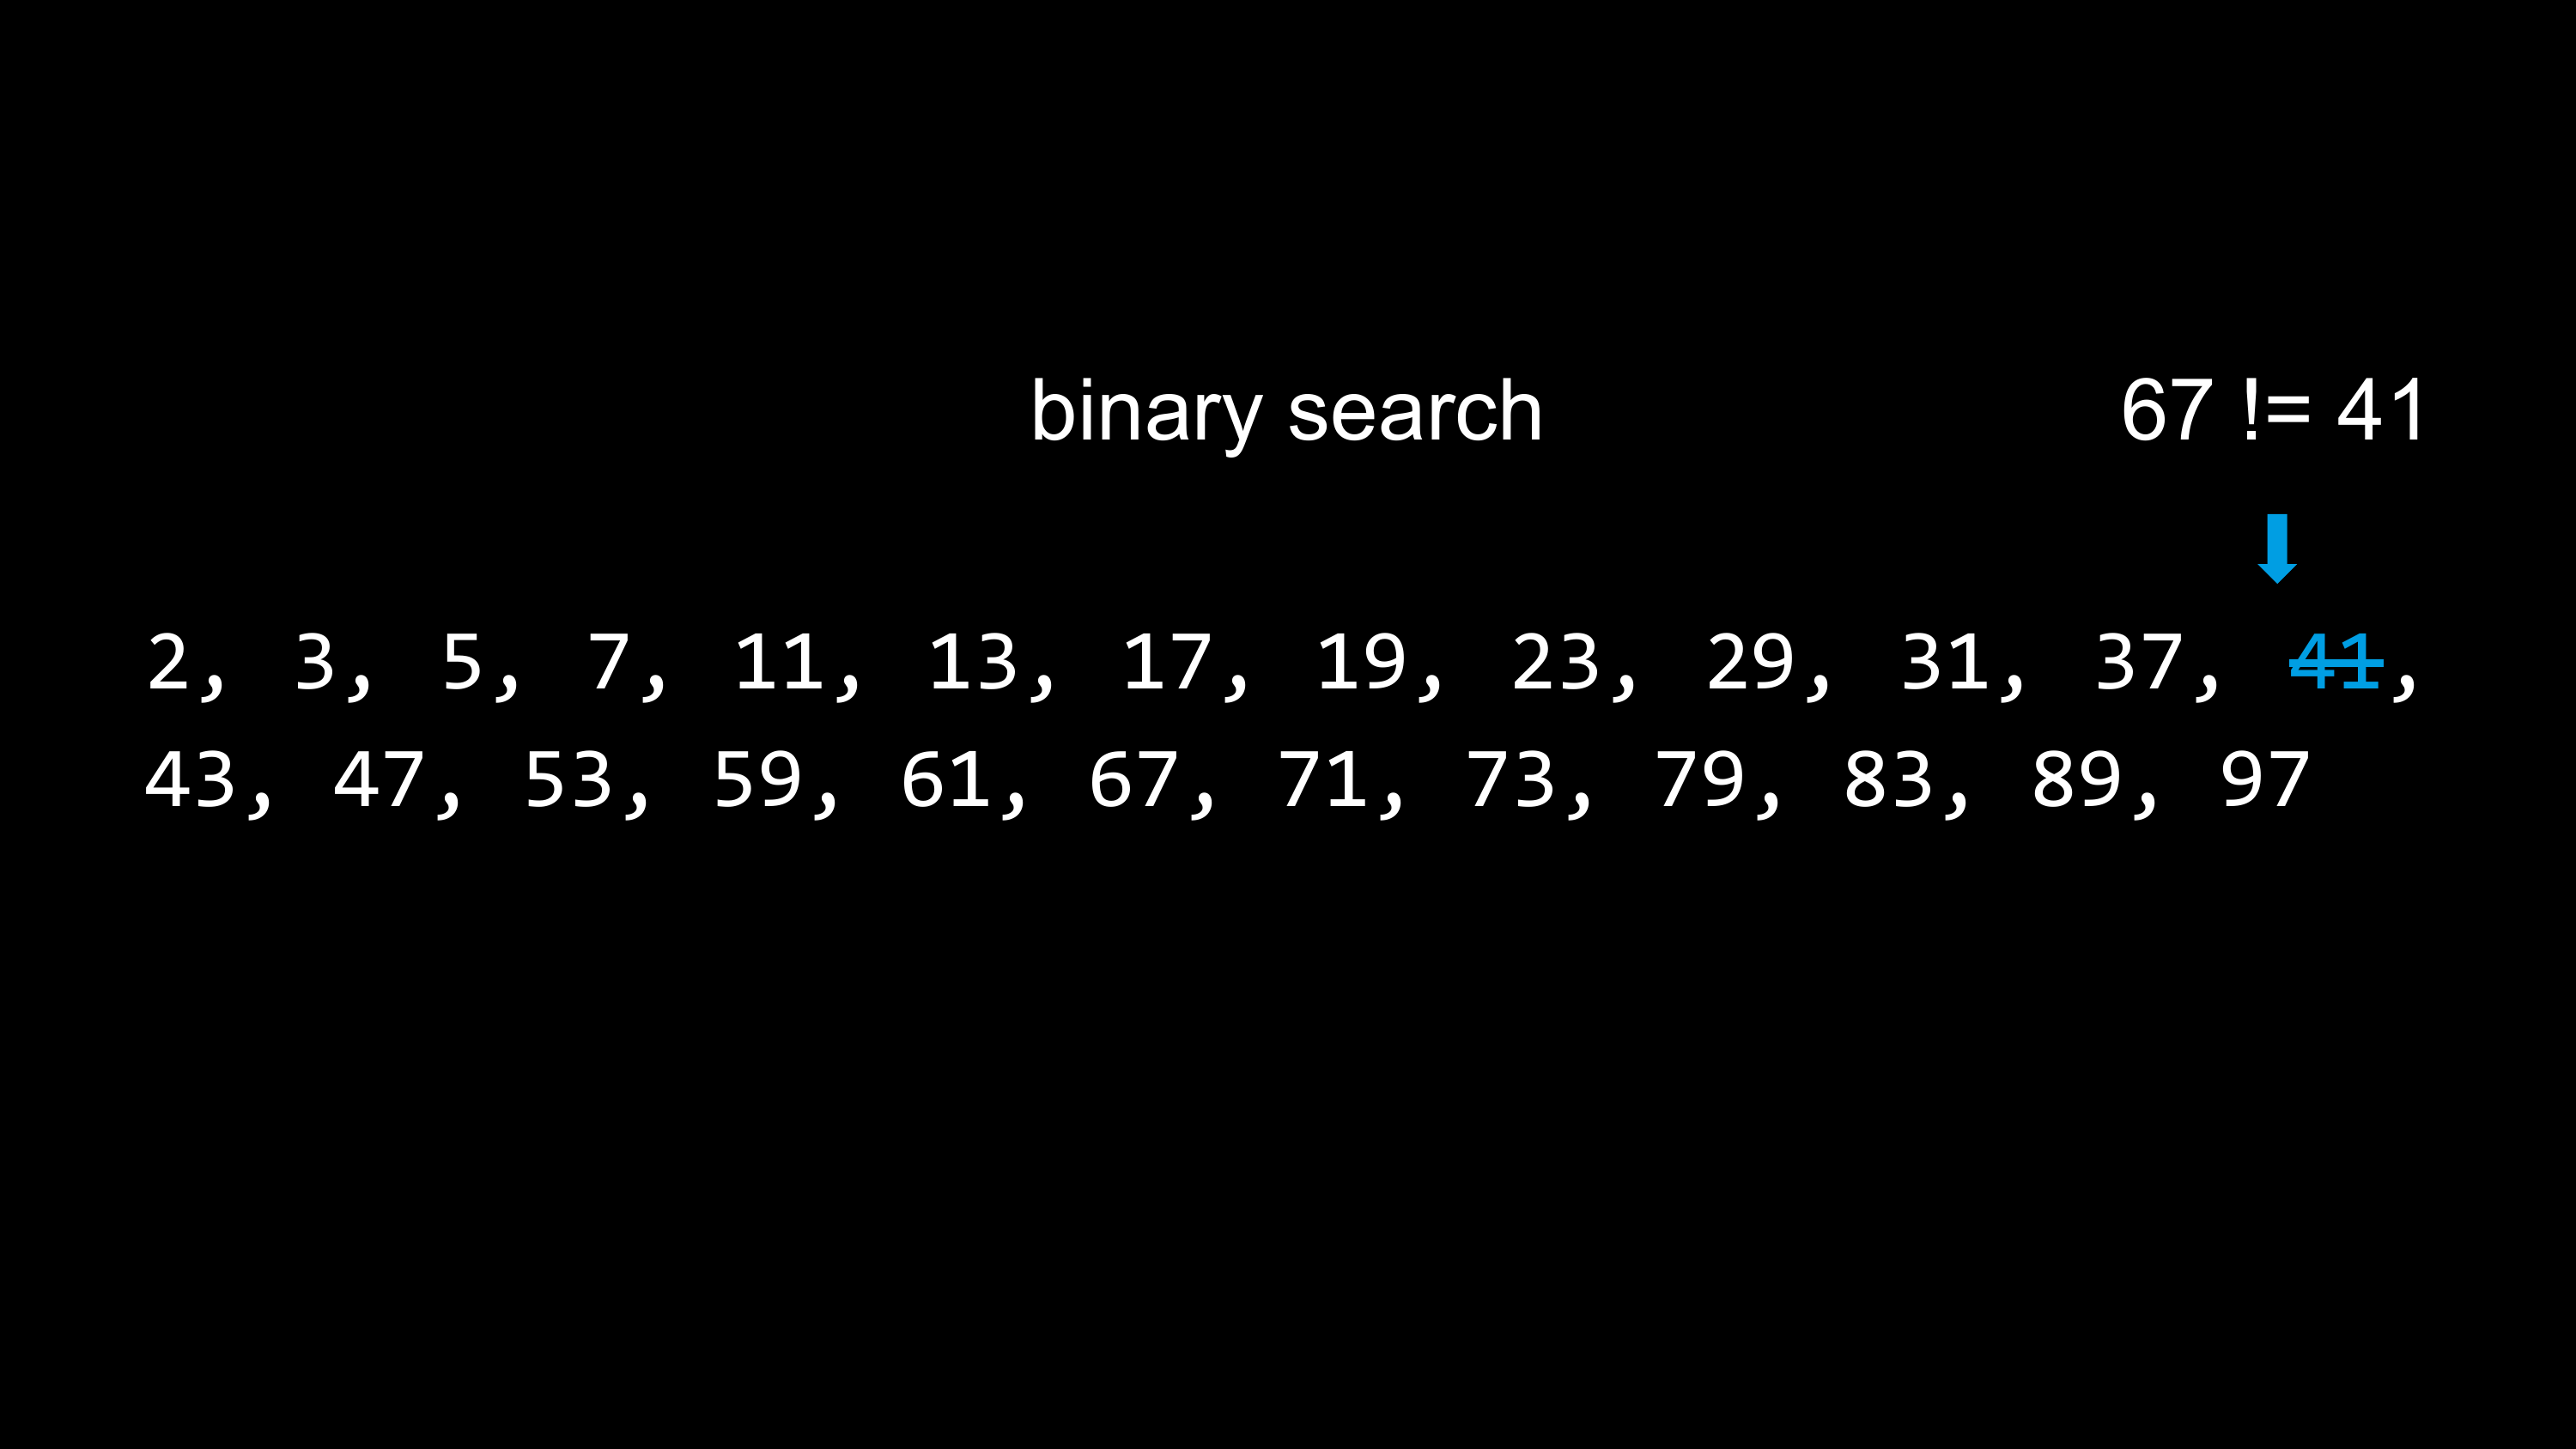
\includegraphics[width=1\linewidth,height=\textheight,keepaspectratio]{problem-solving_files/mediabag/problem_solving_67_p.png}
\end{center}

\subsection{\texorpdfstring{Verteile und Parallelisiere
(\emph{Distribute and
Parallelize})}{Verteile und Parallelisiere (Distribute and Parallelize)}}\label{verteile-und-parallelisiere-distribute-and-parallelize}

Manche Probleme lassen sich effizienter lösen, wenn mehrere Personen
gleichzeitig daran arbeiten. Anstatt eine einzelne Person mit der
gesamten Aufgabe zu betrauen, verteilen wir die Arbeit auf mehrere
Schultern und arbeiten parallel an der Lösung. Allerdings eignet sich
nicht jedes Problem für diesen Ansatz.

Ein gutes Beispiel ist das Aufräumen eines Zimmers: Eine einzelne Person
müsste nacheinander verschiedene Bereiche aufräumen, während mehrere
Personen gleichzeitig unterschiedliche Ecken des Raums in Angriff nehmen
können. Je größer das Zimmer, desto mehr Personen werden benötigt, um es
in der gleichen Zeit aufzuräumen. Ein Gegenbeispiel, bei dem diese
Strategie nicht funktioniert, ist das Lösen einer mathematischen
Gleichung. Hier müssen die einzelnen Rechenschritte aufeinander
aufbauen, weshalb das Problem nicht gleichzeitig an mehrere Personen
übergeben werden kann, die unabhängig daran arbeiten.

Die Strategie des Verteilens und Parallelisierens -- im Englischen
\emph{Distribute and Parallelize} -- funktioniert nach einem klaren
Prinzip: Wir zerlegen ein großes Problem in Teile, die unabhängig
voneinander gelöst werden können. Diese Teile weisen wir dann
verschiedenen Ressourcen zu -- zum Beispiel mehreren Personen oder
Computern. Jede Ressource arbeitet an ihrem Teilproblem und erzeugt ein
eigenes Ergebnis. Dabei gehen wir davon aus, dass sich alle
Teilergebnisse am Ende zu einer Gesamtlösung zusammenfügen lassen.
Ähnlich wie beim Divide and Conquer-Ansatz sind die Teilprobleme meist
gleichartig.

Um dieses Konzept greifbar zu machen, schauen wir uns ein konkretes
Beispiel an, das wir mit dem EVA-Modell analysieren: das Zählen aller
Wörter in einem Buch.

\begin{figure}[H]

{\centering 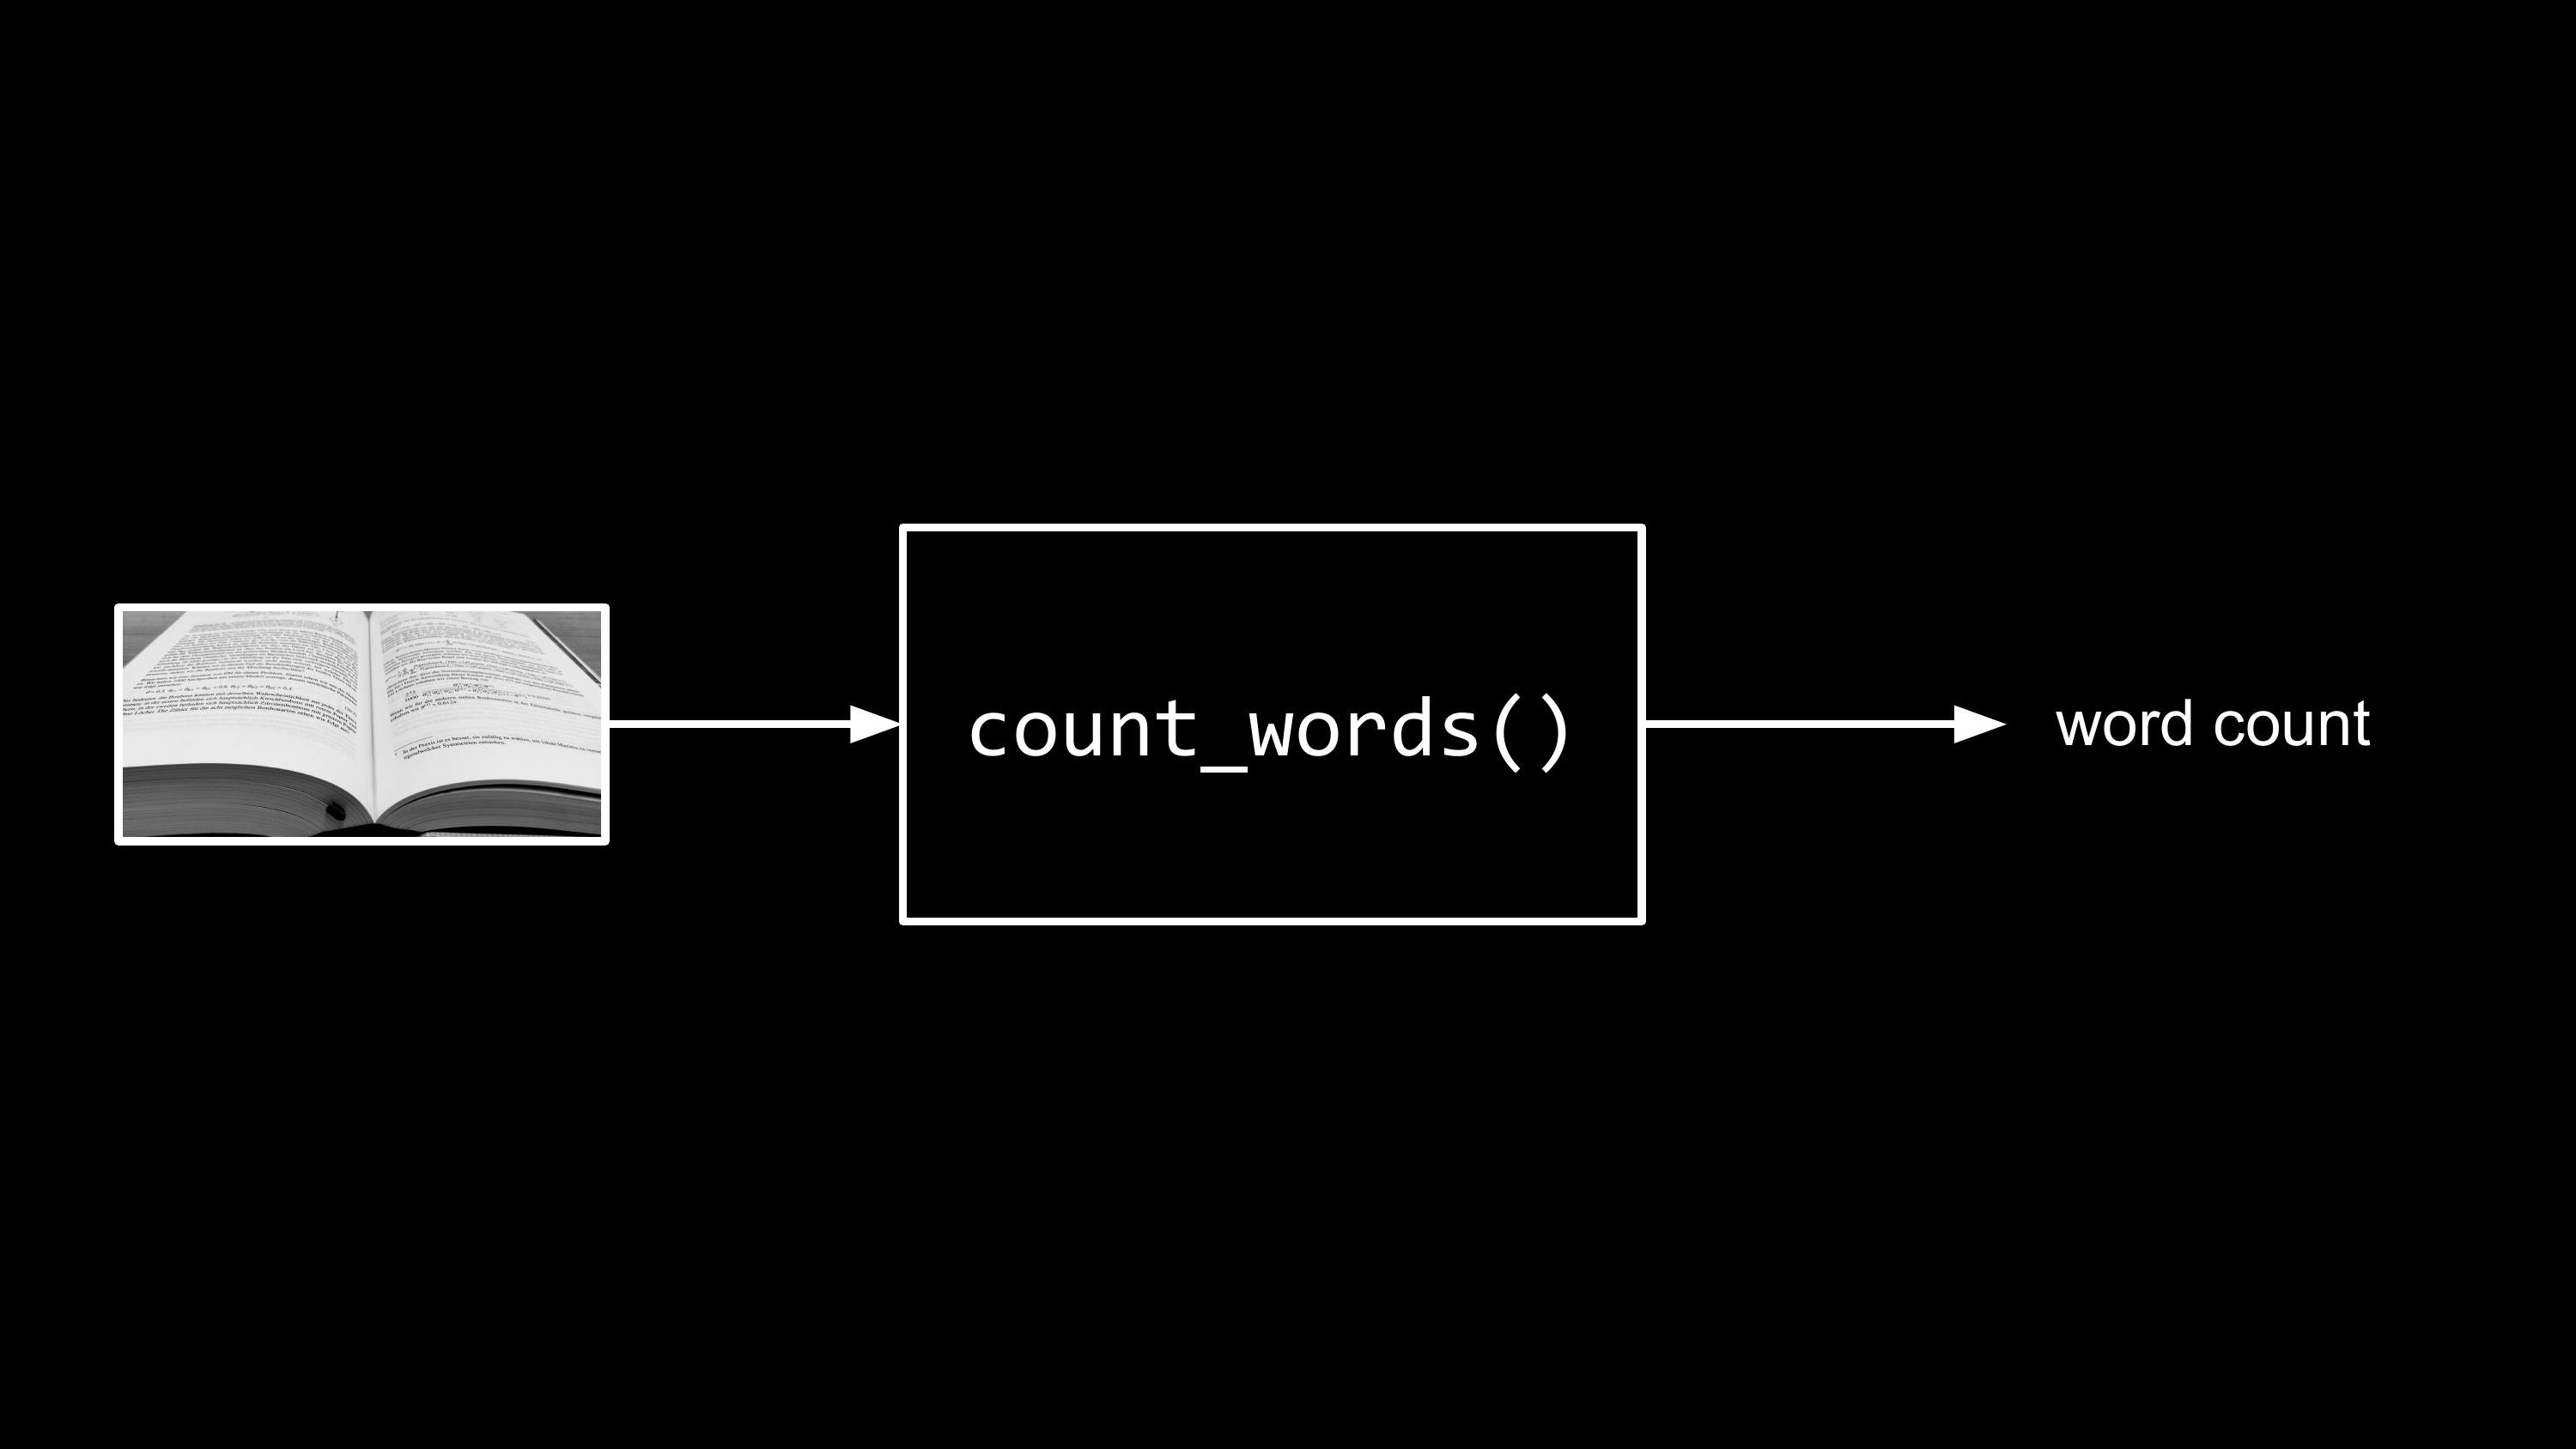
\includegraphics[width=1\linewidth,height=\textheight,keepaspectratio]{problem-solving_files/mediabag/problem_solving_exam1234567.png}

}

\caption{Das Wörterzählen-Problem im EVA-Modell}

\end{figure}%

Je nach Umfang des Buches kann dies eine mühsame Aufgabe sein, besonders
für Menschen. Ein Computer bewältigt ein einzelnes Buch dank seiner
hohen Verarbeitungsgeschwindigkeit problemlos. Allerdings lässt sich das
Problem beliebig erweitern -- etwa wenn wir statt eines Buches alle
Texte im Internet oder sämtliche Wikipedia-Artikel analysieren möchten.
In solchen Fällen wird die Aufgabe auch für Computer aufwendig und
zeitintensiv. Eine Lösung besteht darin, mehrere Computer parallel
einzusetzen.

In Abbildung~\ref{fig-problem-solving-word-count-distributed} sehen wir
beispielhaft die Verteilung der Buchseiten auf vier Studenten. Jeder
erhält einen gleichen Anteil, wodurch sich die Bearbeitungszeit im
Optimalfall auf ein Viertel reduziert. Bei Computern können wir analog
vorgehen und mehrere Rechner gleichzeitig mit Teilen der Seiten
betrauen. Diese Rechner werden in einem Netzwerk verbunden und von einem
zentralen Computer gesteuert, der die Teilergebnisse am Ende
zusammenführt. Ein solches System nennen wir Rechencluster, bestehend
aus Arbeitern -- den \emph{Worker Nodes} -- sowie einer Steuereinheit,
die in solchen Systemen als \emph{Driver} oder \emph{Name Node}
bezeichnet wird.

\begin{figure}

\centering{

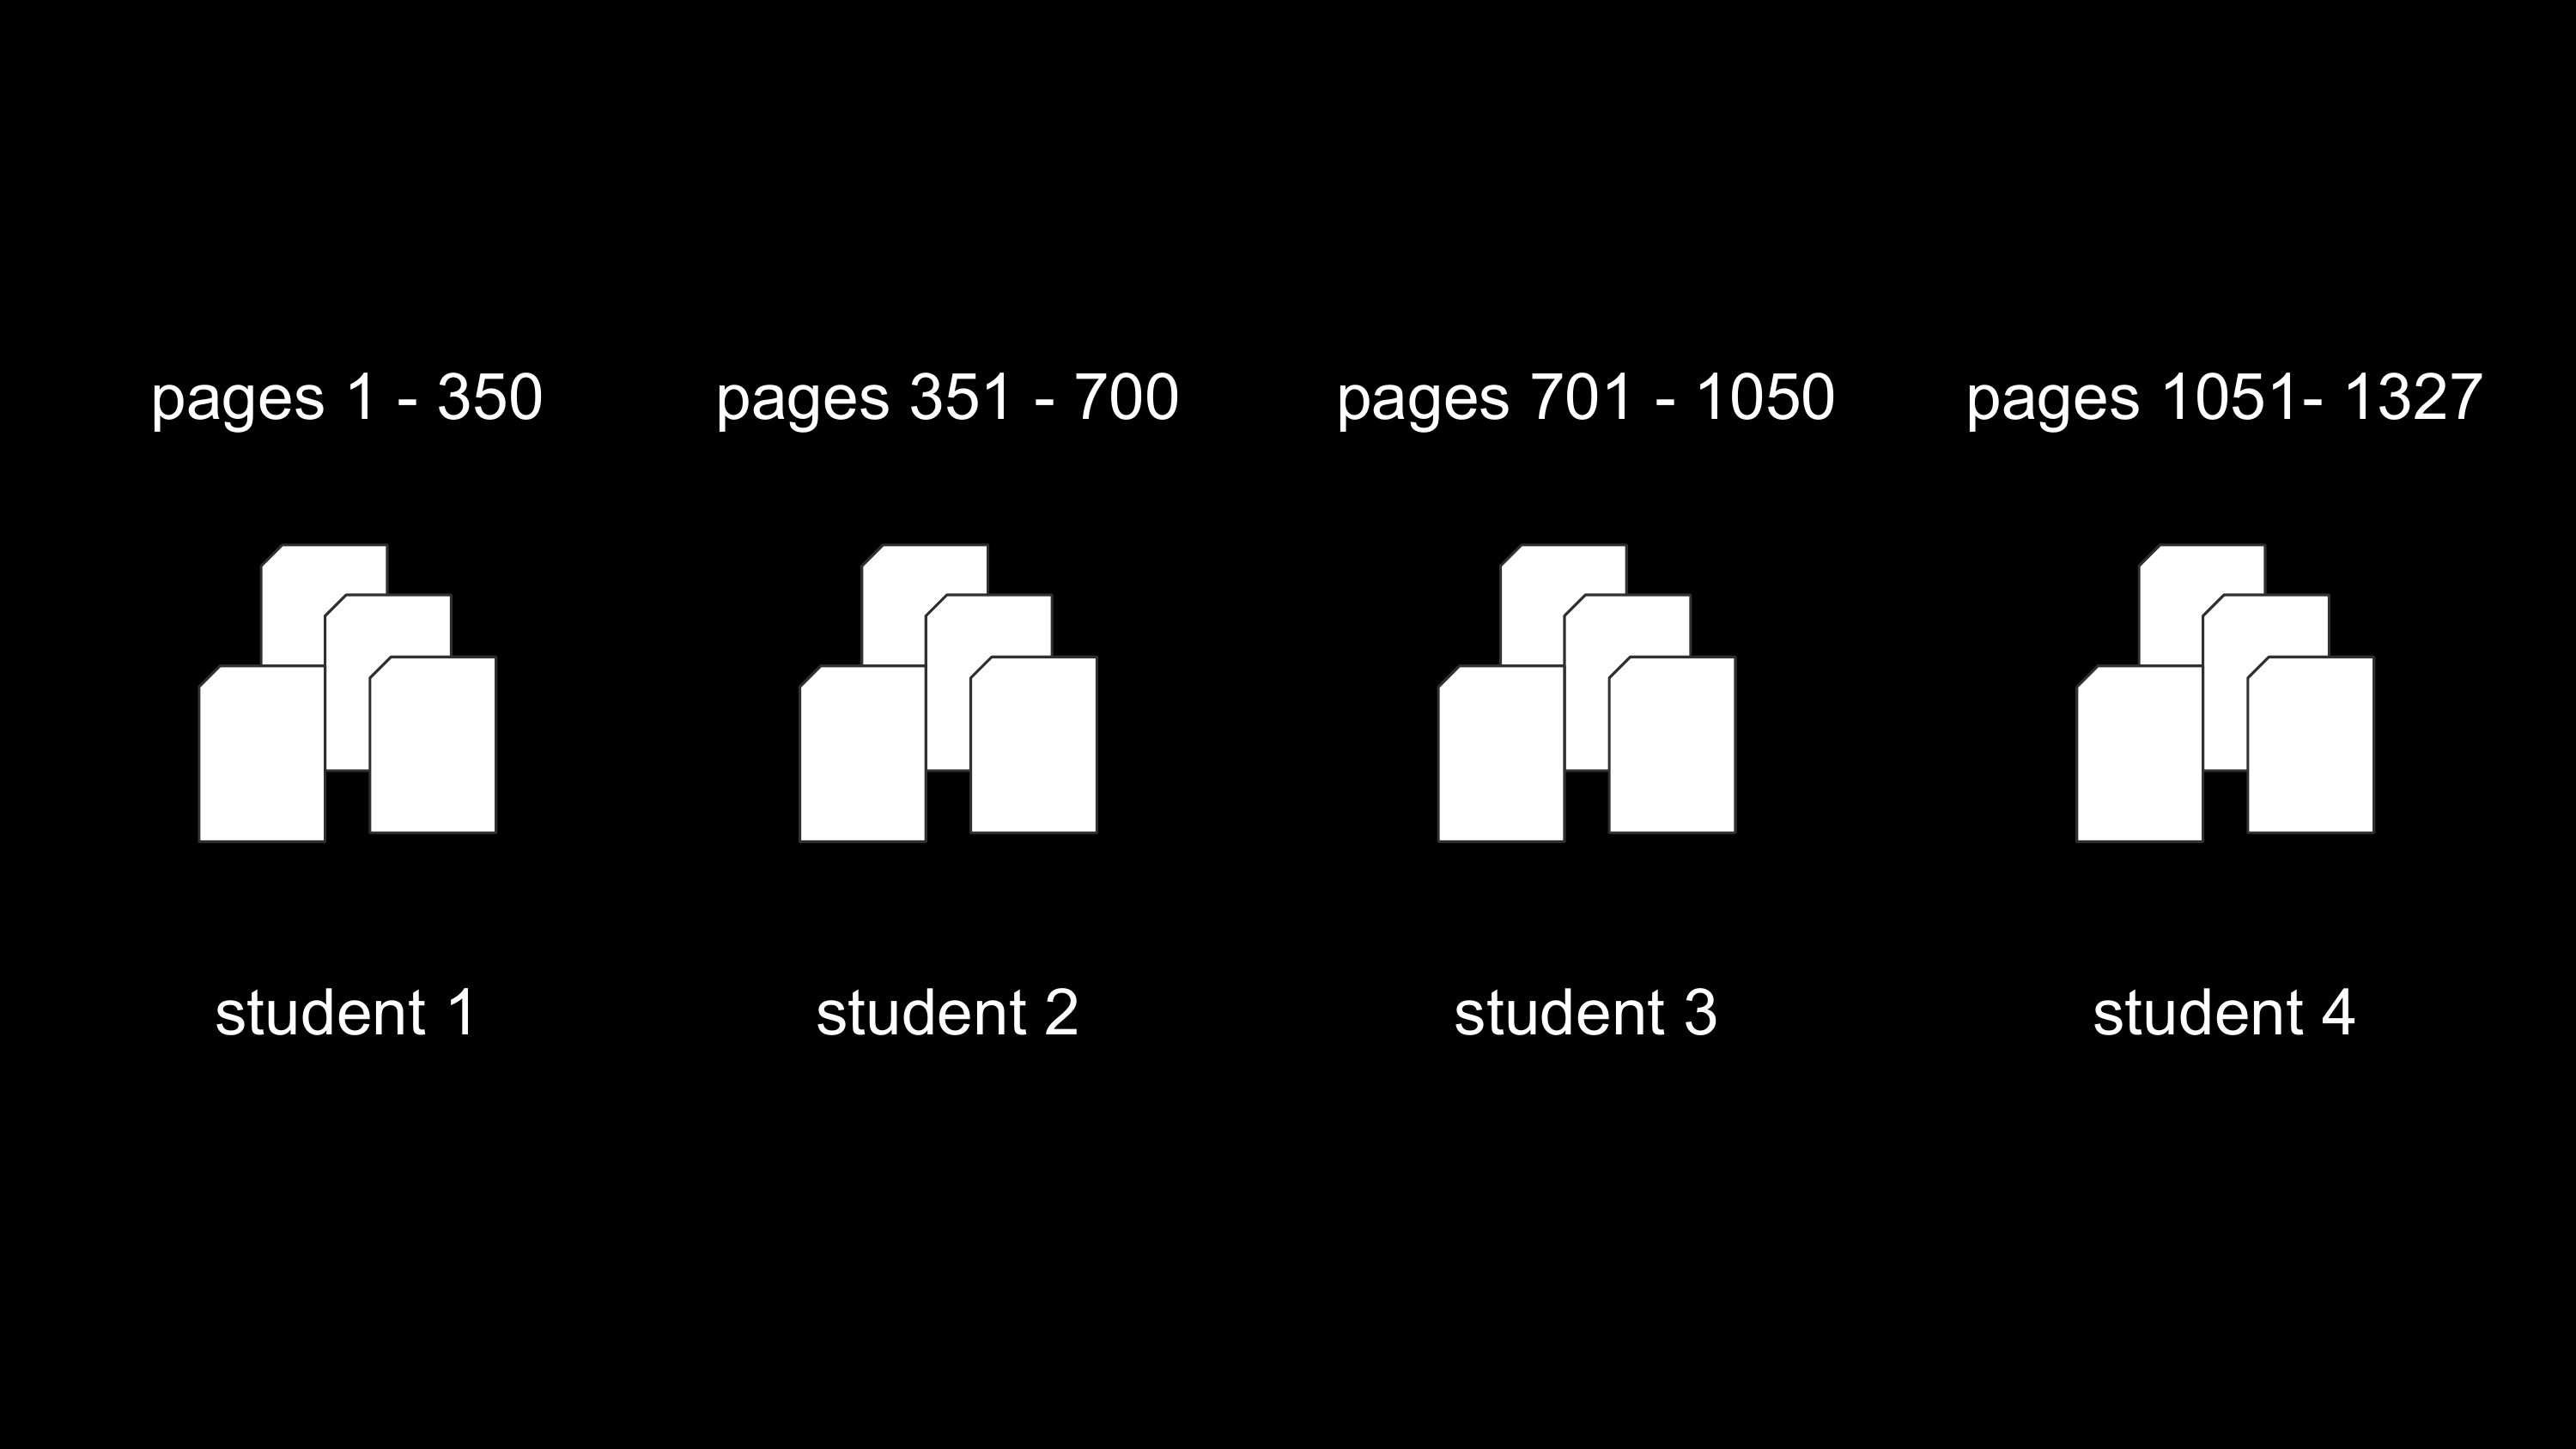
\includegraphics[width=1\linewidth,height=\textheight,keepaspectratio]{problem-solving_files/mediabag/problem_solving_exam12345678.png}

}

\caption{\label{fig-problem-solving-word-count-distributed}Verteiltes
Wörterzählen}

\end{figure}%

Durch die Verteilung und parallele Ausführung kann das EVA-Modell wie in
Abbildung~\ref{fig-eva-distributed} angepasst und detaillierter
dargestellt werden. Statt eines einzelnen Prozesses
\texttt{count\_words} laufen nun \(n\) parallele Prozesse, die jeweils
einen Teil des Buches durchsuchen. Die Aufteilung erfolgt zu Beginn
durch den \texttt{split}-Prozess, während das Zusammenführen der
Teilergebnisse -- in diesem Fall das Addieren der Teilsummen -- durch
den \texttt{merge}-Schritt erfolgt.

\begin{figure}

\centering{

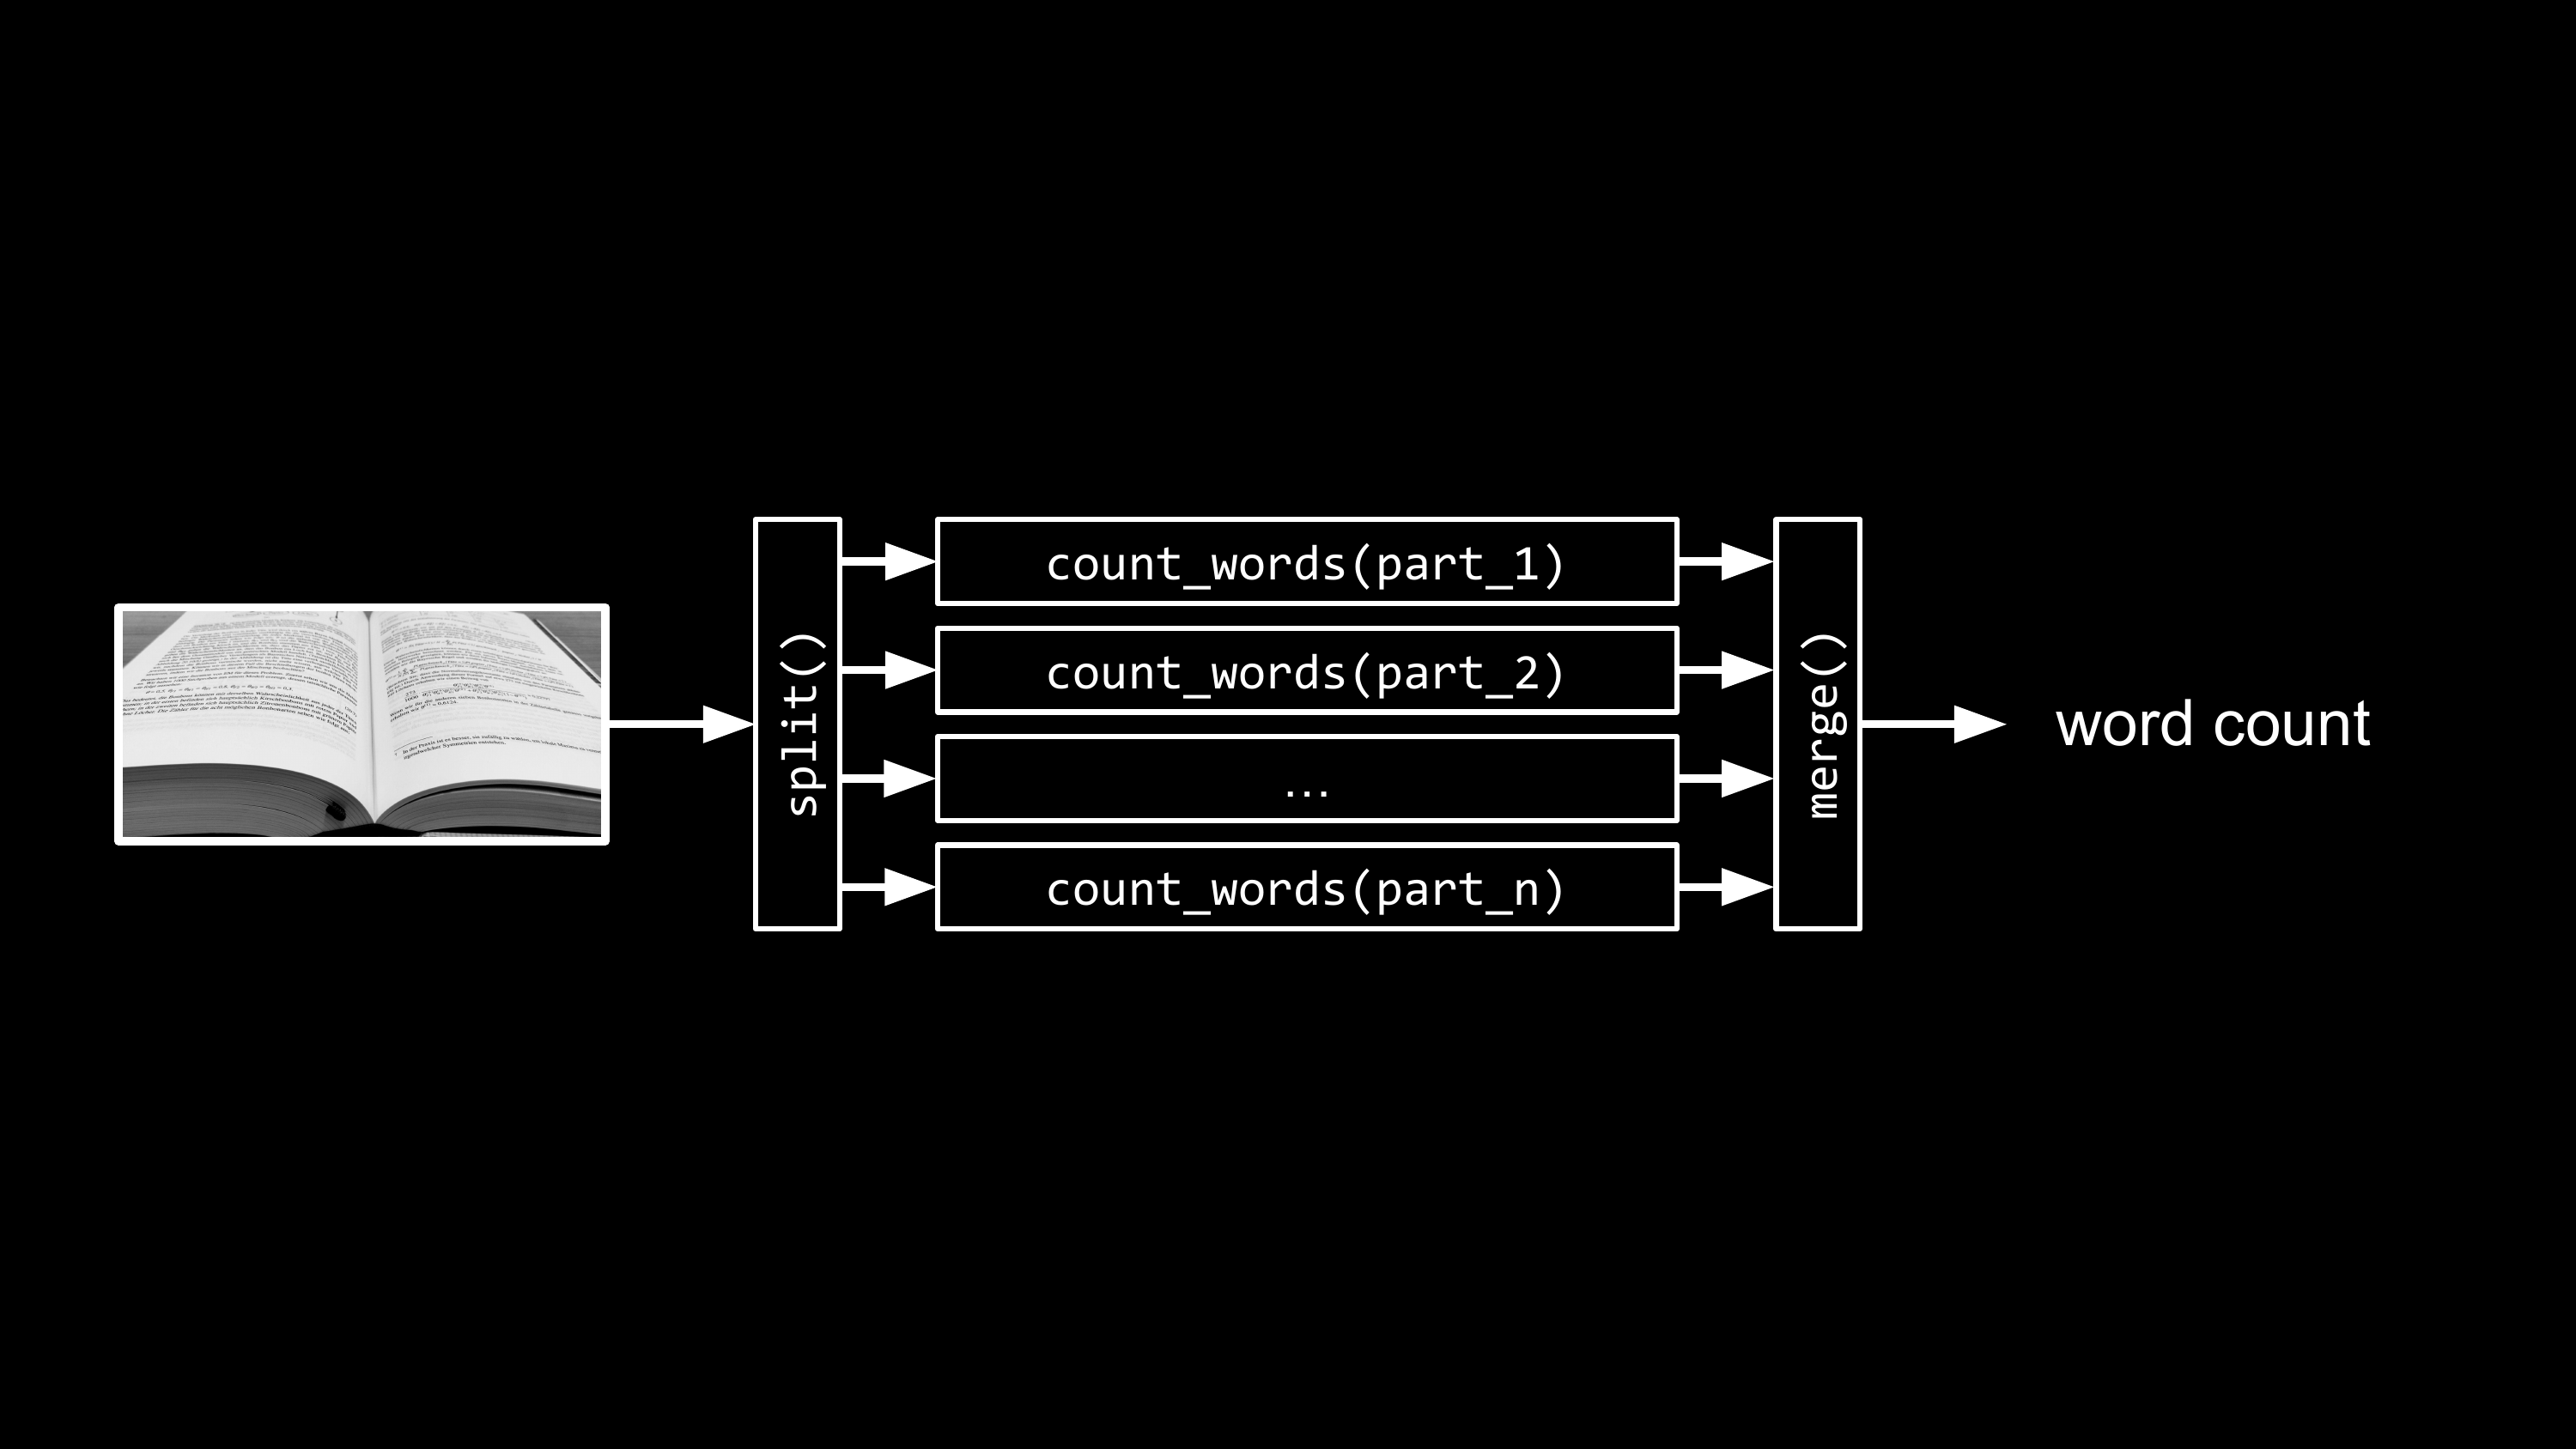
\includegraphics[width=1\linewidth,height=\textheight,keepaspectratio]{problem-solving_files/mediabag/problem_solving_exam123456789.png}

}

\caption{\label{fig-eva-distributed}Das parallelisierte Wörterzählen im
EVA-Modell}

\end{figure}%

In diesem Kapitel haben wir uns mit dem EVA-Modell auseinandergesetzt -
einem fundamentalen Konzept für die computergestützte Problemlösung.
Dieses Modell bietet uns einen strukturierten Rahmen, der aus drei
wesentlichen Komponenten besteht:

\begin{itemize}
\tightlist
\item
  \textbf{Eingabe (E)}: Die zu verarbeitenden Daten oder Informationen
\item
  \textbf{Verarbeitung (V)}: Der Kern der Problemlösung durch
  Algorithmen
\item
  \textbf{Ausgabe (A)}: Das Ergebnis der Verarbeitung in nutzbarer Form
\end{itemize}

Die Verarbeitung als zentrales Element des Modells ist dabei der Ort, an
dem die eigentliche Problemlösung stattfindet. Hier kommen Algorithmen
zum Einsatz - präzise Handlungsanweisungen, die Schritt für Schritt zur
Lösung führen. Die genaue Natur dieser Algorithmen, ihre
charakteristischen Eigenschaften und wie wir sie entwickeln können,
werden wir im nächsten Kapitel detailliert betrachten.

\phantomsection\label{refs}
\begin{CSLReferences}{1}{0}
\bibitem[\citeproctext]{ref-polya}
Pólya, George, und John Horton Conway. 2004. \emph{How to solve it: a
new aspect of mathematical method}. Expanded Princeton Science Library
ed. Princeton science library. Princeton {[}N.J.{]}: Princeton
University Press.

\end{CSLReferences}




\end{document}
